%-----------------------------------------------------------------------------
\documentclass[12pt,a4paper]{report}
%---------------------------------------------------------------------------
\usepackage{amsmath}
\usepackage{amssymb}
\usepackage{amsthm}
\usepackage{amsfonts}
\usepackage{array}
\usepackage{longtable}
\usepackage{appendix}
\usepackage{blkarray}
\usepackage{bibentry}
\usepackage[none]{hyphenat}
\usepackage[noadjust]{cite}
\usepackage{filecontents}
\usepackage[all,knot,arc,poly]{xy}
\usepackage[pdftex]{graphicx}
\graphicspath{{images/}{../images/}}
\DeclareGraphicsExtensions{.pdf,.jpeg,.png, .jpg}
\usepackage{lscape}
\usepackage{epsfig}
\usepackage{mathrsfs}
\usepackage[left=40mm,right=25mm,top=25mm,bottom=25mm]{geometry}
\usepackage{url}
\usepackage{multicol}
\usepackage{multirow}
\usepackage{color}
\usepackage[table]{xcolor}
\definecolor{pink}{rgb}{1,0.5,0.5}
\usepackage{graphicx}
\graphicspath{ {images/} }
\usepackage{float}
\floatstyle{boxed} 
\restylefloat{figure}

\usepackage{tikz}
\usetikzlibrary{patterns,graphs,arrows.meta,shapes,trees,bending,fadings,quotes,angles}





\usepackage{pgfplots}
\usepgfplotslibrary{fillbetween}
\pgfplotsset{compat=1.18}

\usepackage{rotating}
%-----------------------------------------------------------------------------
\usepackage{setspace}
\usepackage{titletoc}
\titlecontents{chapter}
[0pt]
{\bfseries}
{\MakeUppercase\chaptername\ \thecontentslabel:\quad}
{\MakeUppercase}
{\hfill\contentspage}[]
%-----------------------------------------------------------------------------
\usepackage{float}
\textwidth 6.5in \textheight 9.175in\topmargin 0in \headheight 0in
\oddsidemargin 0in \evensidemargin 0in
\parskip 0.5\baselineskip
\parindent 0pt
\renewcommand{\baselinestretch}{1.25}
%-----------------------------------------------------------------------------
\theoremstyle{definition}
\newtheorem{thm}{Theorem}[section]
\newtheorem{definition}[thm]{Definition}
\newtheorem{example}[thm]{Example}
\newtheorem{exe}[thm]{Exercise}
\newtheorem{note}[thm]{Note}
\newtheorem{remark}[thm]{Remark}
\theoremstyle{plain}
\newtheorem{prop}[thm]{Proposition}
\newtheorem{conj}[thm]{Conjecture}
\newtheorem{coro}[thm]{Corollary}
\newtheorem{lem}[thm]{Lemma}
\newtheorem{tech}{Technique}[section]
\newtheorem{fact}[thm]{Fact}
\renewcommand{\contentsname}{TABLE OF CONTENTS}
\renewcommand\bibname{REFERENCES}
%\renewcommand{\qedsymbol}{$\blacksquare$}

\parindent 0ex

%-----------------------------------------------------------------------------
\usepackage{titlesec}
\titleformat{\chapter}[hang]
          {\normalfont\filright\ttfamily\scshape\sffamily\bfseries
          	\centering\large}
          {\MakeUppercase{\chaptertitlename}\ \thechapter}{10pt\ :}{\large\MakeUppercase}        
          \titlespacing*{\chapter}{0pt}{-90pt}{16pt}
                       
\titleformat{\section}[hang]
           {\normalfont\sffamily\bfseries%
            \large}
            {\thesection.}{1ex}{}%[\titlerule]
%-----------------------------------------------------------------------------


%-----------------------------------------------------------------------------
\usepackage{fancyhdr}
\fancyhead{}

\pagestyle{fancy}

\fancyhf{}
%\fancyfoot[C]{\small Prepared by N.~Jeshurun \quad \thepage}

\fancyfoot[C]{\thepage}


%\fancyfoot[C]{\small Prepared by N.~Jeshurun}
\renewcommand{\headrulewidth}{0pt}
\renewcommand{\footrulewidth}{0pt}
%-----------------------------------------------------------------------------

\renewcommand{\sectionmark}[1]{\markright{}} %\thesection\ #1 (this one should be in th brackets, ayoub)
%-----------------------------------------------------------------------------

%-----------------------------------------------------------------------------


\newcommand{\bpf}{\noindent {\ttfamily  PROOF}. $\mbox{}$}
\newcommand{\epf}{\hfill \hbox{\raisebox{.5ex}{$\blacksquare$}$\phantom{.}$}}
%-----------------------------------------------------------------------------

\newtheorem{problemx}{Problem}[section]
\newenvironment{problem}[1]
  {\begin{problemx}\textup{\small[#1]}\hspace{0.4em}\ignorespaces}
  {\end{problemx}}
\newenvironment{solution}
  {\renewcommand{\qedsymbol}{}\begin{proof}[\textit{Solution}.]}
  {\end{proof}}

% tex4ht expands amssymb's \checkmark in TEXT mode and hands MathJax the raw
% internals, so the reader sees \m@th \mathchar"458 instead of a tick.
% \ensuremath forces maths mode, where the token survives.
\let\amscheckmark\checkmark
\renewcommand{\checkmark}{\ensuremath{\amscheckmark}}

\begin{document}
\pagenumbering{roman}
\begin{titlepage}
\thispagestyle{empty}
\begin{center}
\vspace*{4cm}
{\Huge\bfseries Mathematical Statistics}\\[1.2cm]
{\large Lecture Notes}\\[3cm]
\line(1,0){300}
\end{center}
\clearpage
\pagenumbering{roman}
\end{titlepage}
%\maketitle












%----------------------------------------------------------------------------------------------------------------------------------------------------

\newpage
%\phantom{.}
%\vspace{20mm}
%\noindent
%Table of contents
\begin{spacing}{1.7}
\tableofcontents
\addcontentsline{toc}{chapter}{TABLE of CONTENTS}
\end{spacing}

\newpage
%\noindent
%\begin{center}
%{\Large\bf Index of Notation} 
%\end{center}

















\newpage
\pagenumbering{arabic}


%--------------------------------------------------------------------------------------------------------------------------------



\chapter{Probability Distribution of Functions Of Random Variables}

\section{Preliminaries}
\vspace{-15pt}
In mathematical statistics, we often transform one or more random variables to create new variables. For example, if $X_1, X_2, \dots, X_n$ represent a sample, the sample mean $\bar{X} = \frac{1}{n}\sum X_i$ is a function of those variables. To understand the behavior of $\bar{X}$, we must first master the properties of the underlying distributions.



\subsection{Probability Mass and Density Functions}
\vspace{-15pt}
We categorize our variables into two distinct worlds: the discrete and the continuous.

\textbf{1. Discrete PMF:} A function $f_X(x, \theta) = P(X=x)$ for a countable set of values. It must satisfy:$$ f_X(x, \theta) \geq 0 \quad \text{and} \quad \sum_{i} f_X(x_i, \theta) = 1 $$
\textbf{2. Continuous PDF:} For a continuous variable $X$, the probability at a single point is zero. Instead, we define the density such that:$$ f_X(x, \theta) \geq 0 \quad \text{and} \quad \int_{-\infty}^{\infty} f_X(x, \theta) , dx = 1 $$


\subsection{The Cumulative Distribution Function (CDF)}
\vspace{-15pt}
The CDF is the "bridge" between discrete and continuous worlds. It is defined as:$$ F_X(x) = P(X \leq x)$$ 
\textbf{Properties:}
\begin{enumerate}
\item \textbf{Monotonicity:} If $a < b$, then $F_X(a) \leq F_X(b)$.
\item \textbf{Boundary Limits:} $F_X(-\infty) = 0$ and $F_X(+\infty) = 1$.
\item \textbf{Right-Continuity:} $\lim_{h \to 0^+} F_X(x+h) = F_X(x)$.
\end{enumerate}



\subsection{The Moment Generating Function (MGF)}
\vspace{-15pt}
The MGF is a powerful tool because it uniquely identifies a distribution. If two variables have the same MGF, they have the same distribution.$$ M_X(t) = E\left[e^{tX}\right] $$
\textbf{The ``Moment-Generating" Property:} To find the $m^{th}$ moment about the origin ($E[X^m]$), we differentiate the MGF $m$ times and evaluate at $t=0$:$$ E(X^m) = \left. \frac{d^m}{dt^m} M_X(t) \right|_{t=0} $$




\subsection{Multivariate Distributions and Independence}
\vspace{-15pt}
When dealing with functions of variables, we rarely work with just one $X$. We work with vectors $\mathbf{X} = (X_1, X_2, \dots, X_k)^T$.

\begin{definition}
If $X_1,X_2,\cdots X_k$ are $k$ discrete random variables then the joint discrete function denoted by $f_{X_1,X_2,\cdots,X_k}(x_1,x_2,\cdots,x_k,\theta)$ is given by 
\[f_{X_1,X_2,\cdots,X_k}(x_1,x_2,\cdots,x_k,\theta)  = P(X_1=x_1, X_2=x_2,\cdots, X_k=x_k)\] and 
\[\sum\limits_X  P(X_1=x_1,\cdots, X_k=x_k)  = \sum_{X_1}\cdots\sum_{X_k}  P(X_1=x_1,\cdots, X_k=x_k) = 1.\]
\end{definition}




\begin{definition}
If $X_1,X_2,\cdots,X_k$ are $k$ continuous random variables, then the joint pdf denoted by $f_{X_1,X_2,\cdots,X_k}(x_1,x_2,\cdots,x_k,\theta)$, is such that  
\begin{enumerate}
\item $f_{X_1,X_2,\cdots,X_k}(x_1,x_2,\cdots,x_k,\theta)\,\, \geq \, 0 \,\,$ for all $\,\, X = (x_1, x_2, \cdots, x_k)^t$
\item $\int\limits_X   f_{X_1,X_2,\cdots ,X_k}(x_1,x_2,\cdots,x_k,\theta)\,\,  dX = 1$ 
$$\int_{X_1}\int_{X_2}\cdots\int_{X_k} f_{X_1,X_2,\cdots,X_k}(x_1,x_2,\cdots,x_k,\theta)dx_k\, dx_{k-1}\cdots dx_1$$
\end{enumerate}
\end{definition}




\begin{definition}
The random variables $X_1,X_2,\cdots,X_k$ (discrete or continuous) are stochastically independent if and only if 
\begin{align*}
f_{X_1,X_2,\cdots,X_k}(x_1,x_2,\cdots,x_k) & = f_{X_1}(x_1)\, f_{X_2}(x_2)\, \cdots\, f_{X_k}(x_k)\\
 & = \prod^k_{j=1} f_{X_j} (x_j)
\end{align*} where $f_{X_j}(x_j)$ is the marginal probability function $j = 1,2,\cdots, k$.
\end{definition}







\subsection{Joint Moment Generating Functions}
\vspace{-15pt}
The joint MGF allows us to handle sums of random variables with ease.

\begin{definition}
The joint moment generating function of  $X_1, X_2 , \cdots,X_k$ denoted by $M_{X_1, X_2,  \cdots, X_k} (t_1, t_2,\cdots, t_k)$ is given by 
\begin{align*}
M_{\textbf{X}} (\textbf{t})  & = E\left(e^{x_1t_1 +  \cdots x_kt_k}\right)\\
& = E\left[e^{\sum\limits^k_{j=1}x_jt_j}\right]\\
& = E\left[\prod^k_{j=1}e^{x_jt_j}\right]\\
& = E\left[e^{XT}\right].
\end{align*}
\end{definition}



\begin{thm}
Random variables $X_1,X_2,\cdots,X_k$ are stochastically independent if and only if the joint moment generating function is a product of the MGFs of the marginals 
\begin{align*}
M_{X_1,\cdots, X_k} (t_1,\cdots, t_k) & = M_{X_1}(t_1)\, \cdots\, M_{X_k}(t_k)\\
& = \prod^k_{j=1} M_{X_j}(t_j).
\end{align*}
\end{thm}





\subsection{Properties of the Bivariate CDF}
\vspace{-15pt}
For a bivariate distribution, the probability that $(X_1, X_2)$ falls within a rectangle $[a,b] \times [c,d]$ is: 
$$ P(a \leq X_1 \leq b, c \leq X_2 \leq d) = F(b,d) - F(b,c) - F(a,d) + F(a,c).$$
\begin{figure}[H]
\centering
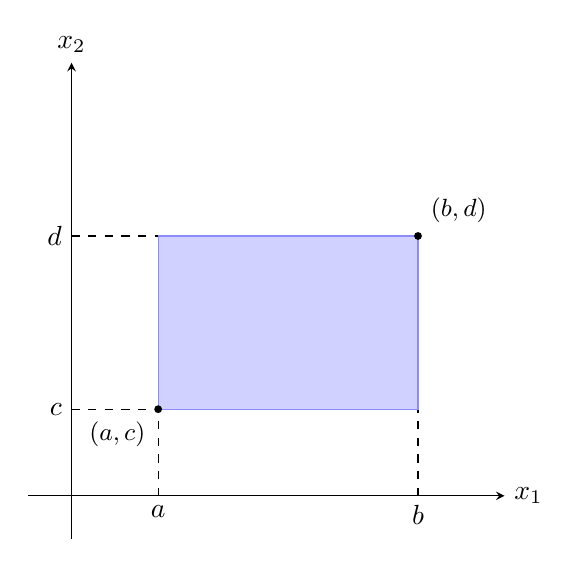
\begin{tikzpicture}[scale=1.1, >=stealth]
\draw[->] (-0.5,0) -- (5,0) node[right] {$x_1$};
\draw[->] (0,-0.5) -- (0,5) node[above] {$x_2$};
\draw[dashed] (1,0) node[below] {$a$} -- (1,3);
\draw[dashed] (4,0) node[below] {$b$} -- (4,3);
\draw[dashed] (0,1) node[left] {$c$} -- (4,1);
\draw[dashed] (0,3) node[left] {$d$} -- (4,3);

\filldraw[fill=blue!18, draw=blue!45] (1,1) rectangle (4,3);

\node[circle, fill=black, inner sep=1pt, label=above right:{\small $(b,d)$}] at (4,3) {};
\node[circle, fill=black, inner sep=1pt, label=below left:{\small $(a,c)$}] at (1,1) {};
\end{tikzpicture}
\caption{The probability of a rectangular region is found by inclusion-exclusion of the Joint CDF values at the vertices.}\end{figure}







%%%%%%%%%%%%%%%%%%%%%%%%%%%%%%%%%%%%%%%%%%%%%%%%%%%%%%%%%%%%%%%%%%
\section{Distribution of Order Statistics}
\vspace{-15pt}
Suppose $X_1, X_2, \dots, X_n$ is a random sample from a population. When we arrange these observations in increasing order of magnitude, we obtain the \textbf{Order Statistics}:$$ X_{(1)} \leq X_{(2)} \leq \dots \leq X_{(n)} $$ We often denote these as $Y_1, Y_2, \dots, Y_n$ to distinguish them from the raw sample.

\begin{itemize}
\item $Y_1 = \min(X_1, \dots, X_n)$ is the first (smallest) order statistic.
\item $Y_n = \max(X_1, \dots, X_n)$ is the largest order statistic.
\item $Y_{(n+1)/2}$ (for odd $n$) represents the sample median.
\end{itemize}


%%%%%%%%%%%%%%%%%%%%%%%%%%%%%%%%%%%%%%%%%%%%%%
\subsection{The Joint PDF}
\vspace{-15pt}
\begin{thm}
If $X_1, X_2, \cdots\, , X_n$ is a random sample from a population with continuous PDF $f(x)$, then the joint PDF of the order statistics $Y1, Y_2, \cdots, \, Y_n$ is given by
$$ f(y_1, y_2, \dots, y_n) = n! \prod_{i=1}^n f(y_i), \quad\quad -\infty < y_1 < y_2 < \dots < y_n < \infty $$ The $n!$ factor accounts for the fact that any of the $n!$ permutations of the original sample could have resulted in this specific ordered set.
\end{thm}


\begin{example}Suppose that $X_1, X_2, X_3$ represent a random sample of size 3 from an Exponential population with PDF:$$ f(x) = e^{-x}, \quad x > 0 $$ Find: 
\begin{enumerate}
\item[(i).] The joint PDF of the order statistics $Y_1, Y_2, Y_3$.
\begin{proof}[\textbf{\textit{Solution}}]
Using the theorem $f(y_1, y_2, y_3) = n! \prod f(y_i)$:
\begin{align*}
f(y_1, y_2, y_3) &= 3! \, f(y_1) f(y_2) f(y_3)\\
&= 6 (e^{-y_1})(e^{-y_2})(e^{-y_3})\\
&= 6 e^{-(y_1 + y_2 + y_3)}\, , \quad 0 < y_1 < y_2 < y_3 < \infty
\end{align*}
\end{proof}




\item[(ii).] The marginal PDF of $Y_1$ (the minimum).
\begin{proof}[\textbf{\textit{Solution}}]
To find $f(y_1)$, we integrate out $y_3$ (from $y_2$ to $\infty$) and $y_2$ (from $y_1$ to $\infty$):
\begin{align*}
f(y_1) &= \int_{y_1}^{\infty} \int_{y_2}^{\infty} 6e^{-y_1}e^{-y_2}e^{-y_3} \, dy_3 \, dy_2\\
&= 6e^{-y_1} \int_{y_1}^{\infty} e^{-y_2} \left[ -e^{-y_3} \right]_{y_2}^{\infty} \, dy_2\\
&= 6e^{-y_1} \int_{y_1}^{\infty} e^{-y_2} (e^{-y_2}) \, dy_2\\
& = 6e^{-y_1} \int_{y_1}^{\infty} e^{-2y_2}\, dy_2\\
&= 6e^{-y_1} \left[ -\frac{1}{2}e^{-2y_2} \right]_{y_1}^{\infty}\\
& = 6e^{-y_1} \left( \frac{1}{2}e^{-2y_1} \right)\\
& = 3e^{-3y_1}, \quad y_1 > 0.
\end{align*}
\end{proof}


\item[(iii).] The marginal PDF of $Y_3$ (the maximum).
\begin{proof}[\textbf{\textit{Solution}}]
To find $f(y_3)$, we integrate out $y_1$ (from $0$ to $y_2$) and $y_2$ (from $0$ to $y_3$):
\begin{align*}
f(y_3) &= \int_{0}^{y_3} \int_{0}^{y_2} 6e^{-y_1}e^{-y_2}e^{-y_3}\, dy_1\, dy_2\\
&= 6e^{-y_3} \int_{0}^{y_3} e^{-y_2} \left[ -e^{-y_1} \right]_{0}^{y_2}\, dy_2\\
&= 6e^{-y_3} \int_{0}^{y_3} e^{-y_2} (1 - e^{-y_2})\, dy_2\\
& = 6e^{-y_3} \int_{0}^{y_3} (e^{-y_2} - e^{-2y_2})\, dy_2\\
&= 6e^{-y_3} \left[ -e^{-y_2} + \frac{1}{2}e^{-2y_2} \right]_{0}^{y_3}\\
& = 6e^{-y_3} \left( -e^{-y_3} + \frac{1}{2}e^{-2y_3} + 1 - \frac{1}{2} \right)\\
&= 6e^{-y_3} \left( \frac{1}{2} - e^{-y_3} + \frac{1}{2}e^{-2y_3} \right)\\
& = 3e^{-y_3} - 6e^{-2y_3} + 3e^{-3y_3}, \quad y_3 > 0.
\end{align*}
\end{proof}
\end{enumerate}
\end{example}


\subsection{Derivation of Extremes: Minimum and Maximum}
\vspace{-15pt}
The distribution of the maximum and minimum are fundamental in areas like reliability theory and extreme value analysis.

\begin{thm}
Suppose $X_1, X_2, \dots, X_n$ are independent and identically distributed (i.i.d.) continuous random variables with PDF $f_X(x)$ and CDF $F_X(x)$. The PDF of the maximum $Y = X_{(n)}$ and the minimum $U = X_{(1)}$ are derived as follows:
\end{thm}
\begin{proof}
\textbf{1. The Distribution of the Maximum ($Y = X_{(n)}$):} The maximum value of a sample is less than or equal to $y$ if and only if \textbf{every} individual observation is less than or equal to $y$.
\begin{align*}
F_Y(y) &= P(Y \leq y) = P(X_1 \leq y, X_2 \leq y, \dots, X_n \leq y)\\
&= P(X_1 \leq y)P(X_2 \leq y)\dots P(X_n \leq y) \quad (\text{by independence})\\
& =\prod^n_{i = 1}F_{X_i}(y)\\
& = [F_X(y)]^n \quad (\text{since i.i.d.})
\end{align*}
Differentiating with respect to $y$ gives the PDF:$$ f_Y(y) = \frac{d}{dy} [F_X(y)]^n = n[F_X(y)]^{n-1} f_X(y) $$
\textbf{2. The Distribution of the Minimum ($U = X_{(1)}$):} The minimum is greater than $u$ if and only if \textbf{every} individual observation is greater than $u$.
\begin{align*}
F_U(u) &= P(U \leq u) = 1 - P(U > u)\\
&= 1 - P(X_1 > u, X_2 > u, \dots, X_n > u)\\
&= 1 - [P(X_1 > u)]^n \quad (\text{by independence and identical distribution})\\
&= 1 - [1 - F_X(u)]^n.
\end{align*}
Differentiating with respect to $u$:$$ f_U(u) = \frac{d}{du} (1 - [1 - F_X(u)]^n) = n[1 - F_X(u)]^{n-1} f_X(u) $$
\end{proof}




\subsection{The $k^{\text{th}}$ Order Statistic}
\vspace{-15pt}
Having derived the boundaries, we now present the general theorem for any $k^{\text{th}}$ value in the ordered sequence.

\begin{note}
To understand the PDF of $Y_k$, imagine a number line representing the support of our distribution. We pick a point $y$. For $Y_k$ to be exactly at $y$, the $n$ observations must fall into three distinct bins:
\begin{enumerate}
\item $k-1$ observations must fall to the \textbf{left} of $y$ (each with probability $F(y)$).
\item Exactly \textbf{one} observation must fall at the point $y$ (density $f(y)$).
\item The remaining $n-k$ observations must fall to the \textbf{right} of $y$ (each with probability $1-F(y)$).
\end{enumerate}
\begin{figure}[H]
\centering
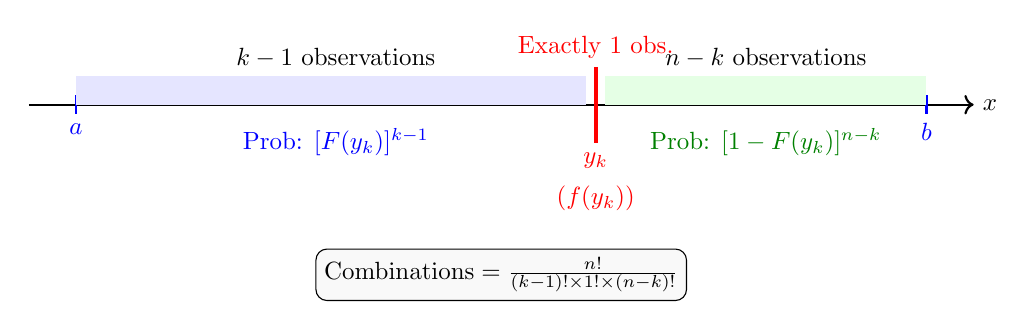
\begin{tikzpicture}[scale=1.2, every node/.style={scale=0.9}]
% Draw the number line
\draw[thick, ->] (0,0) -- (10,0) node[right] {$x$};
% Draw the intervals
\draw[blue, thick] (0.5, 0.1) -- (0.5, -0.1) node[below] {$a$};
\draw[blue, thick] (9.5, 0.1) -- (9.5, -0.1) node[below] {$b$};

% The point y_k
\draw[red, ultra thick] (6, 0.4) -- (6, -0.4) node[below] {$y_k$};
\node[red, above] at (6, 0.4) {Exactly 1 obs.};
\node[red] at (6, -0.99) {($f(y_k)$)};

% Left Region
\fill[blue!10] (0.5, 0) rectangle (5.9, 0.3);
\node at (3.25, 0.5) {$k-1$ observations};
\node[blue] at (3.25, -0.4) {Prob: $[F(y_k)]^{k-1}$};

% Right Region
\fill[green!10] (6.1, 0) rectangle (9.5, 0.3);
\node at (7.8, 0.5) {$n-k$ observations};
\node[green!50!black] at (7.8, -0.4) {Prob: $[1-F(y_k)]^{n-k}$};

% Multinomial Coefficient
\node[draw, rounded corners, fill=gray!5] at (5, -1.8) {$\text{Combinations} = \frac{n!}{(k-1)! \times 1! \times (n-k)!}$};
\end{tikzpicture}\caption{The spatial partitioning of a sample for the $k^{th}$ order statistic.}
\end{figure}
\end{note}










\begin{thm}Let $X_1, X_2, \dots, X_n$ denote a random sample of size $n$ from a continuous population with PDF $f(x)$ supported on $(a, b)$. The PDF of the $k^{\text{th}}$ order statistic $Y_k$ is:$$ f(y_k) = \frac{n!}{(k - 1)!(n - k)!} [F_X(y_k)]^{k-1} [1 - F_X(y_k)]^{n - k} f(y_k) $$for $a < y_k < b$, and zero otherwise.\end{thm}


\begin{exe} In Example 1.2.2, we derived the marginal PDFs for the minimum ($Y_1$) and the maximum ($Y_3$) of an Exponential sample size $n=3$ using double integration.Now, use the Order Statistic Theorem formula to directly find the PDFs for:
\begin{enumerate}
\item[(i).] The sample minimum, $Y_1 = X_{(1)}$.
\item[(ii).] The sample median, $Y_2 = X_{(2)}$.
\item[(iii).] The sample maximum, $Y_3 = X_{(3)}$.
\end{enumerate}
Verify that your results for $Y_1$ and $Y_3$ match the results obtained via integration in the previous example.
\end{exe}





%%%%%%%%%%%%%%%%%%%%%%%%%%%%%%%%%%%%%%%%
\begin{thm}
For a random sample of size $n$ from a discrete or continuous CDF, $F_X(x)$, the marginal CDF of the $k^{\text{th}}$ order statistics is given by \[F(y_k) = \sum^n_{j = k}\binom{n}{j}\left[F_X(y_k)\right]^j\left[1 - F_X(y_k)\right]^{n-j}.\]
\end{thm}


\begin{example}
Let $X_1, X_2, X_3$ be  a random sample from $f(x) = 2x, \quad 0< x  < 1$. Find
\begin{enumerate}
\item[(i).] the CDF of $Y_2 = X_{(2)}$
\begin{proof}[\textbf{\textit{Solution}}]
$f(x) = 2x, \quad 0 < x < 1$
\[F_X(x) = \begin{cases}
0, & x \leq 0\\
x^2, & 0 < x < 1\\
1, & x\geq 
\end{cases}\]

\[F(y_k) = \sum^n_{j = k}\binom{n}{j}\left[F_X(y_k)\right]^j\left[1 - F_X(y_k)\right]^{n-j}\]
\begin{align*}
F(y_2)  &  = \sum^3_{j = 2}\binom{3}{j}\left(y^2_2\right)^j\left[1 - y^2_2\right]^{3-j}\\
& = \binom{3}{2}\left(y^2_2\right)^2\left(1 - y^2_2\right)^1 + \binom{3}{3}\left(y^2_2\right)^3\left(1 - y^2_2\right)^0\\
& = 3y^4_2\left(1 - y^2_2\right) + y^6_2\\
& = y^4_2\left(3 - 2y^2_2\right).
\end{align*}
Therefore
\[F(y_2) = \begin{cases}
0, & y_2 \leq 0\\
y^4_2(3 - 2y^2_2), & 0 < y_2 < 1\\
1, & y\geq 1
\end{cases}\]
\end{proof}


\item[(ii).] the PDF of $Y_2 = X_{(2)}$
\begin{proof}[\textbf{\textit{Solution}}]
We have two pathways to find the PDF.
\begin{itemize}\item \textbf{Pathway A (Derivative of CDF):} $$ f_{Y_2}(y) = \frac{d}{dy} F_{Y_2}(y) = \frac{d}{dy}(3y^4 - 2y^6) = 12y^3 - 12y^5 = 12y^3(1 - y^2) $$
\item \textbf{Pathway B (Direct Formula):} Using $n=3, k=2$: $$ f_{Y_2}(y) = \frac{3!}{1!1!} [y^2]^1 [1 - y^2]^1 (2y) = 6(y^2)(1 - y^2)(2y) = 12y^3(1 - y^2) $$
\end{itemize} 
Both pathways confirm the same result for $0 < y < 1$.
\end{proof}
\end{enumerate}
\end{example}



\subsection{Distribution of the Range}
The \textit{Sample Range} is defined as $R = Y_n - Y_1$. It is a vital measure of dispersion in non-parametric statistics and quality control. While we will use the Jacobian method later to derive its exact PDF for any distribution, we can already state the \textit{Joint PDF of the Extremes} ($Y_1$ and $Y_n$) using the same "multinomial logic" from our diagram:



\begin{thm}
For a random sample of size $n$, the joint PDF of $Y_1$ and $Y_n$ is:$$ f_{Y_1, Y_n}(y_1, y_n) = n(n-1) [F(y_n) - F(y_1)]^{n-2} f(y_1) f(y_n) $$for $a < y_1 < y_n < b$.
\end{thm}





%%%%%%%%%%%%%%%%%%%%%%%%%%%%%%%%%%%%%%%%%%%%%%%%%%%%%
\section{Functions of Random Variables}
\vspace{-15pt}
Suppose $(X_1, X_2, \cdots , X_k)$ are continuous random variables with joint PDF $f(x_1, x_2, \cdots , x_n)$. Our goal is to determine the distribution of a new set of variables $(Y_1, Y_2, \cdots, Y_k)$ which are functions of the original sample:
\begin{align*}
Y_1 & = h_1(X_1, X_2, \cdots, X_n)\\
Y_2 & = h_2(X_1,X_2, \cdots , X_n)\\
\vdots & \\
Y_k & = h_k(X_1, X_2, \cdots , X_n)
\end{align*}

We generally employ three primary techniques: 
\begin{enumerate} 
\item \textbf{The CDF Technique:} Best for single functions or where the geometry of the transformation is easily understood. \item \textbf{The Transformation (Jacobian) Method:} Best for one-to-one multivariate mappings. 
\item \textbf{The Moment Generating Function (MGF) Method:} Most powerful for sums of independent variables. 
\end{enumerate}





\subsection{The Cumulative Distribution Function Method}
\vspace{-15pt}
This method relies on the definition of the CDF. If $Y = g(X)$, we find the probability that $Y \leq y$ (i.e., $F_Y(y) = P(Y \leq y)$)  by identifying the corresponding region in the $X$-space and integrating the original density over that regio



\begin{thm}[\textbf{The CDF Procedure}]
To find the PDF of $Y = g(X_1, \dots, X_n)$:
\begin{enumerate}
\item \textbf{Define the event:} Write $F_Y(y) = P(Y \leq y) = P(g(X_1, \dots, X_n) \leq y)$.
\item \textbf{Integrate:} Evaluate $F_Y(y) = \iint \dots \int_{\mathcal{R}} f(x_1, \dots, x_n) \, dx_1 \dots dx_n$, where $\mathcal{R}$ is the region where $g(\mathbf{x}) \leq y$.
\begin{align*}
F_Y(y) & = P(Y \leq y)\\
& = P(g(X) \leq y)\\
& = P(X \leq g^{-1}(y))\\
& = F_X(g^{-1}(y))
\end{align*}

\item \textbf{Differentiate:} Obtain the PDF by taking the derivative $f_Y(y) = \frac{d}{dy} F_Y(y)$.
\begin{align*}
f_Y(y) & = \frac{d}{dy}F_Y(y)\\
& = f_X(g^{-1}(y))\, \frac{d}{dy}(g^{-1}(y)).
\end{align*}
\end{enumerate}
\end{thm}



\begin{example}
Let $X$ be a continuous random variable and $Y = X^2$. Find the PDF of $Y$.
\end{example}
\begin{proof}[\textbf{\textit{Solution}}] Note that $Y$ can only take non-negative values ($y > 0$).
\begin{align*}F_Y(y)  & = P(Y \leq y) = P(X^2 \leq y)\\
&= P(-\sqrt{y} \leq X \leq \sqrt{y})\\
&= F_X(\sqrt{y}) - F_X(-\sqrt{y})
\end{align*}
Applying the chain rule to differentiate with respect to $y$:
\begin{align*}
f_Y(y) & = \frac{d}{dy} [F_X(\sqrt{y}) - F_X(-\sqrt{y})]\\
& = f_X(\sqrt{y}) \cdot \frac{1}{2\sqrt{y}} - f_X(-\sqrt{y}) \cdot \left(-\frac{1}{2\sqrt{y}}\right)\\
&= \frac{1}{2\sqrt{y}} \left[ f_X(\sqrt{y}) + f_X(-\sqrt{y}) \right], \quad y > 0
\end{align*}
\end{proof}




\begin{example}
Given $f_X(x) = 2e^{-2x}$ for $x > 0$, find the PDF of $Y = e^X$.
\end{example}
\begin{proof}[\textbf{\textit{Solution}}] \textit{Step 1: Find the Population CDF.}  For $x > 0$: $$F_X(x) = \int_0^x 2e^{-2t} dt = 1 - e^{-2x}.$$
\textit{Step 2: Transform.} Since $x > 0$, the range of $Y = e^X$ is $\,(e^0, \infty)$, so $y > 1$.
\begin{align*}
F_Y(y) & = P(e^X \leq y) = P(X \leq \ln y)\\
&= F_X(\ln y)\\
&= 1 - e^{-2(\ln y)}\\
& = 1 - e^{\ln(y^{-2})}\\
& = 1 - y^{-2}, \quad y > 1
\end{align*}
\textit{Step 3: Differentiate.} $$ f_Y(y) = \frac{d}{dy}(1 - y^{-2}) = 2y^{-3}, \quad y > 1 $$
\end{proof}




\begin{example}
Let $X$ be a random sample from a Uniform distribution on the interval $(0, 1)$, such that:$$ f_X(x) = 1, \quad 0 < x < 1 $$Define the transformation $Y = -2\ln X$. Find the PDF of $Y$. 
\end{example}
\begin{proof}[\textbf{\textit{Solution}}]\textit{Step 1: Determine the support of $Y$.}Since $0 < x < 1$, we evaluate the boundaries:
\begin{itemize}
\item As $x \to 1$, $Y = -2\ln(1) = 0$.
\item As $x \to 0^+$, $Y = -2\ln(0^+) \to \infty$.
\end{itemize}
Thus, the support of $Y$ is $y > 0$.

\textit{Step 2: Find the CDF $F_Y(y)$.}
\begin{align*}F_Y(y) &= P(Y \leq y)\\
&= P(-2\ln X \leq y)\\
&= P\left(\ln X \geq -\frac{y}{2}\right) \quad \text{(Note: Inequality flips when dividing by -2)}\\
& = P\left(X \geq e^{-y/2}\right)\\
&= 1 - P\left(X < e^{-y/2}\right)\\
&= 1 - F_X(e^{-y/2})
\end{align*}
Since $F_X(x) = x$ for a Uniform $(0,1)$ distribution:$$ F_Y(y) = 1 - e^{-y/2}, \quad y > 0 $$
\textit{Step 3: Find the PDF $f_Y(y)$ by differentiation.}
\begin{align*}
f_Y(y) &= \frac{d}{dy} \left[ 1 - e^{-y/2} \right]\\
&= 0 - \left( e^{-y/2} \cdot -\frac{1}{2} \right)\\
&= \frac{1}{2} e^{-y/2}, \quad y > 0.
\end{align*}
\end{proof}


\begin{remark}
``Does this resulting PDF look familiar?"
\begin{enumerate}
\item It is an Exponential Distribution with $\lambda = 1/2$.
\item Even more importantly, this is a Chi-square distribution with 2 degrees of freedom ($\chi^2_{(2)}$).
\end{enumerate}
\end{remark}







%%%%%%%%%%%%%%%%%%%%%%%%%%%%%%%%%%%%%%%%

















\subsection{Transformation (Change of Variable) Method}
\subsubsection{1. The Discrete Case} 
\vspace{-15pt}
In the discrete world, transformation is straightforward because we are simply re-labeling the points in the sample space.

\begin{thm}[\textbf{Discrete Case}] Suppose $X$ is a discrete random variable with PF $f_X(x)$. If $Y = g(X)$ is a one-to-one transformation with inverse $x = g^{-1}(y)$, then the PF of $Y$ is:$$ f_Y(y) = f_X(g^{-1}(y)), \quad y \in \text{Support of } Y $$
\end{thm}


\begin{example} 
If $X \sim \text{Geo}(p)$, where $f_X(x) = pq^{x-1}$ for $x = 1, 2, 3, \dots$, find the distribution of $Y = X - 1$.
\end{example}
\begin{proof}[\textbf{\textit{Solution}}] 
The inverse is $x = y + 1$. Substituting this into the original PF:$$ f_Y(y) = f_X(y+1) = pq^{(y+1)-1} = pq^y, \quad y = 0, 1, 2, \dots $$
\textit{Expert Note: This shifts the "Geometric" distribution from counting the trial of the first success to counting the number of failures before the first success.}
\end{proof}


\subsubsection{2. The Continuous Case (Univariate)}
\vspace{-15pt}
In the continuous case, we cannot just re-label points; we must account for the change in density.

\begin{thm}[\textbf{Continuous Case}] Let $X$ have PDF $f_X(x)$. If $Y = h(X)$ is a one-to-one transformation with a continuous, non-zero derivative, the PDF of $Y$ is: $$ f_Y(y) = f_X(h^{-1}(y)) \cdot \left| \frac{d}{dy}h^{-1}(y) \right|$$ where $J = \frac{dx}{dy}$ is the Jacobian of the transformation.
\end{thm}



\begin{example}
Suppose $X$ follows a \textit{Beta distribution} with parameters $\alpha$ and $\beta$. Find the PDF of $Y = -\ln X$. $$ f_X(x) = \frac{1}{B(\alpha, \beta)} x^{\alpha - 1}(1 - x)^{\beta - 1}, \quad 0 < x < 1$$
\end{example}

\begin{proof}[\textbf{\textit{Solution}}]
Determine the Support of $Y$: Since $X \in (0, 1)$:
\begin{itemize}
\item As $x \to 1$, $y = -\ln(1) = 0$.
\item As $x \to 0^+$, $y = -\ln(0^+) \to \infty$.
\end{itemize}
Thus, $Y \in (0, \infty)$.

Find the Inverse Transformation: $$ y = -\ln x \implies -y = \ln x \implies x = e^{-y} $$So, $h^{-1}(y) = e^{-y}$.

Calculate the Jacobian:$$ J = \frac{dx}{dy} = \frac{d}{dy}(e^{-y}) = -e^{-y} $$
The absolute value of the Jacobian is $|J| = e^{-y}$.

Substitute into the Transformation Formula: $f_Y(y) = f_X(h^{-1}(y)) \cdot |J|$:
\begin{align*}
f_Y(y) & = \frac{1}{B(\alpha, \beta)} (e^{-y})^{\alpha - 1} (1 - e^{-y})^{\beta - 1} \cdot e^{-y}\\
& = \frac{1}{B(\alpha, \beta)} e^{-y\alpha + y} (1 - e^{-y})^{\beta - 1} e^{-y}\\
& = \frac{1}{B(\alpha, \beta)} e^{-\alpha y} (1 - e^{-y})^{\beta - 1}, \quad y > 0
\end{align*}
\end{proof}




\subsubsection{3. Bivariate Transformations}
\vspace{-15pt}
When we move to two dimensions (e.g., finding the distribution of the sum or ratio of two variables), we must use the bivariate Jacobian.

\begin{definition}[\textbf{Bivariate Transformation}]
Let $(X, Y)$ have joint PDF $f_{X,Y}(x,y)$. Let $U = h_1(X,Y)$ and $V = h_2(X,Y)$ be a one-to-one transformation with inverses $x = w_1(u,v)$ and $y = w_2(u,v)$. The joint PDF of $(U, V)$ is:$$ f_{U,V}(u,v) = f_{X,Y}(w_1(u,v), w_2(u,v)) \cdot |J| $$where the Jacobian $J$ is the determinant:$$ J = \frac{\partial(x,y)}{\partial(u,v)} = \begin{vmatrix} \frac{\partial x}{\partial u} & \frac{\partial x}{\partial v} \\ \frac{\partial y}{\partial u} & \frac{\partial y}{\partial v} \end{vmatrix}.$$
\end{definition}



\begin{example}
Let $X\thicksim \operatorname{GAM}(a,1)$ and $Y\thicksim\operatorname{GAM}(b,1)$. Suppose $X$ and $Y$ are independent.
\begin{enumerate}
\item[(i).] Find the joint p.d.f. of $U = X + Y$ and $V = \frac{X}{X + Y}$.
\begin{proof}[\textit{\textbf{Solution}}]
$X\thicksim\operatorname{GAM}(\alpha,\beta)$ 
\[f_X(x) = \frac{1}{\beta^{\alpha}\Gamma(\alpha)}\, x^{\alpha - 1}\, e^{-\frac{x}{\beta}}\, , \quad x > 0\]
now $X\thicksim \operatorname{GAM}(a,1)$
\[f_X(x) = \frac{1}{\Gamma(a)}\, x^{a - 1}\, e^{-x}\, , \quad x > 0\]
$Y\thicksim \operatorname{GAM}(b,1)$
\[f_Y(y)  = \frac{1}{\Gamma(b)}\, y^{b-1}\, e^{-y}\,, \quad y > 0\]
Since $X, Y$ are independent, their joint PDF is the product of their marginals:$$ f_{X,Y}(x,y) = \frac{1}{\Gamma(a)\Gamma(b)} x^{a-1} y^{b-1} e^{-(x+y)}, \quad x, y > 0 $$We define the transformation $u = x + y$ and $v = x/(x+y)$. The inverse functions are:$$ x = uv \quad \text{and} \quad y = u(1-v) $$The support of the new variables is $u > 0$ and $0 < v < 1$. 


\begin{figure}[H]
\centering
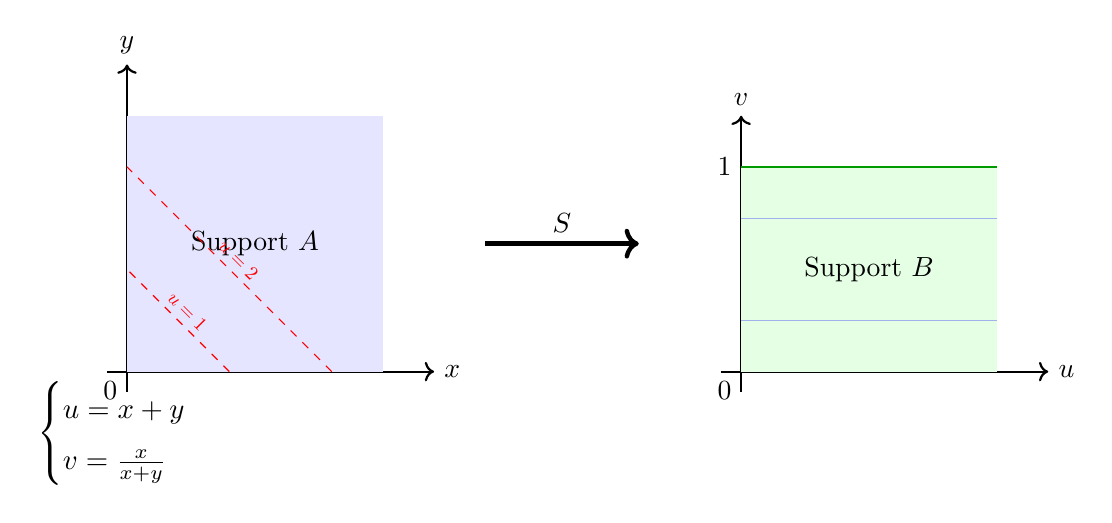
\begin{tikzpicture}[scale=1.3]
    % Left Plane (X,Y)
    \draw[->, thick] (-0.2,0) -- (3,0) node[right] {$x$};
    \draw[->, thick] (0,-0.2) -- (0,3) node[above] {$y$};
    \fill[blue!10] (0,0) rectangle (2.5,2.5);
    \node at (1.25, 1.25) {Support $A$};
    \node[below left] at (0,0) {$0$};
    
    % Dashed lines representing U = x+y
    \draw[dashed, red] (1,0) -- (0,1) node[midway, sloped, above, scale=0.7] {$u=1$};
    \draw[dashed, red] (2,0) -- (0,2) node[midway, sloped, above, scale=0.7] {$u=2$};
    
    % Transformation Arrow
    \draw[->, ultra thick] (3.5, 1.25) -- (5, 1.25) node[midway, above] {$S$};
    \node[midway, below, scale=0.8] at (4.25, 1.2) {$\begin{cases} u=x+y \\ v=\frac{x}{x+y} \end{cases}$};

    % Right Plane (U,V)
    \begin{scope}[shift={(6,0)}]
        \draw[->, thick] (-0.2,0) -- (3,0) node[right] {$u$};
        \draw[->, thick] (0,-0.2) -- (0,2.5) node[above] {$v$};
        
        % Rectangular Support
        \fill[green!10] (0,0) rectangle (2.5, 2);
        \draw[thick, green!60!black] (0,2) -- (2.5, 2);
        \node[left] at (0,2) {$1$};
        \node[below left] at (0,0) {$0$};
        \node at (1.25, 1) {Support $B$};
        
        % Horizontal lines corresponding to constant v
        \draw[blue, opacity=0.3] (0, 0.5) -- (2.5, 0.5);
        \draw[blue, opacity=0.3] (0, 1.5) -- (2.5, 1.5);
    \end{scope}
\end{tikzpicture}
\caption{The transformation maps the $x,y > 0$ quadrant to a rectangular strip where $u > 0$ and $0 < v < 1$.}
\end{figure}

The Jacobian is:$$ J = \begin{vmatrix} \frac{\partial x}{\partial u} & \frac{\partial x}{\partial v} \\ \frac{\partial y}{\partial u} & \frac{\partial y}{\partial v} \end{vmatrix} = \begin{vmatrix} v & u \\ 1-v & -u \end{vmatrix} = -uv - u(1-v) = -u $$Taking the absolute value, $|J| = u$. Substituting into the joint PDF formula:
\begin{align*}
f_{U,V}(u,v) & = f_{X,Y}(uv, u(1-v)) \cdot u\\
& = \frac{1}{\Gamma(a)\Gamma(b)} (uv)^{a-1} (u(1-v))^{b-1} e^{-u} \cdot u\\
&= \frac{1}{\Gamma(a)\Gamma(b)} u^{a+b-1} e^{-u} v^{a-1} (1-v)^{b-1}
\end{align*}
\end{proof}



\item[(ii).] Are $U$ and $V$ independent random variables.
\begin{proof}[\textit{\textbf{Solution}}]
\begin{align*}
f_{U,V}(u,v) & = u^{a + b - 1} e^{-u}\, \frac{v^{a - 1}(1 - v)^{b - 1}}{\Gamma(a)\Gamma(b)}\\
& = \underbrace{\frac{u^{a + b - 1} e^{-u}}{\Gamma(a + b)}}_{f_U(u)} \, \times \, \underbrace{\frac{\Gamma(a + b)\, v^{a - 1}(1 - v)^{b - 1}}{\Gamma(a)\Gamma(b)}}_{f_V(v)}\, , \quad\quad u>0, \, 0 < v < 1
\end{align*}
support is rectangular $\{u: \, u>0\}\times \{v:\, 0 < v < 1\}$.

Therefore, by the factorization theorem of independence $U$ and $V$ are independent.
\end{proof}



\item[(iii).] Find the marginal PDF of $U$ and the marginal PDF of $V$.

\begin{proof}[\textit{\textbf{Solution}}]
\begin{align*}
f_U(u) & = \int_vf_{U,V}(u,v)\, dv\\
& = \int^1_0u^{a + b - 1} e^{-u}\,\frac{v^{a - 1}(1 - v)^{b-1}}{\Gamma(a)\Gamma(b)}\, dv\\
& = \frac{u^{a + b -1}e^{-u}}{\Gamma(a)\Gamma(b)}\int^1_0v^{a-1}(1- v)^{b - 1}\, dv\\
& = \frac{u^{a + b - 1}e^{-u}}{\Gamma(a)\Gamma(b)}\, \frac{\Gamma(a)\Gamma(b)}{\Gamma(a + b)}\\
& = \frac{u^{a + b - 1} \, e^{-u}}{\Gamma(a + b)}\, , \quad\quad u > 0\quad \text{i.e.}\quad U\thicksim \operatorname{GAM}(a + b ,1).
\end{align*}

\begin{align*}
f_V(v) & = \int_uf_{U,V}(u,v)\, du\\
& = \int^{\infty}_0 u^{a + b - 1}e^{-u}\, \frac{v^{a - 1} (1 - v)^{b - 1}}{\Gamma(a)\Gamma(b)}\, du\\
& = \frac{v^{a - 1}(1 - v)^{b - 1}}{\Gamma(a)\Gamma(b)} \int^{\infty}_0u^{a + b -1}e^{-u}\, du\\
& = \frac{v^{a - 1}(1 - v)^{b - 1}}{\Gamma(a)\Gamma(b)}\,\Gamma(a + b)\\
& = \frac{v^{a - 1}\, (1 - v)^{b - 1}}{B(a,b)}\, , \quad 0 < v < 1.
\end{align*}
i.e. $\, V \thicksim \operatorname{BETA}(a,b)$.
\end{proof}
\end{enumerate}
\end{example}



\begin{exe}
Show that 
\begin{enumerate}
\item $E[V] = \frac{a}{a+b}$.
\item $\text{Var}(V) = \frac{ab}{(a+b)^2(a+b+1)}$.
\item $E[U] = a+b$ and $\text{Var}(U) = a+b$.
\end{enumerate}
\end{exe}


\subsubsection{4. Discrete Bivariate Transformations}
\vspace{-15pt}
In the discrete case, we simply perform a point-to-point mapping. The key challenge for learners is usually correctly identifying the new support (the bounds of the summation).

\begin{definition}
Suppose $f(x,y)$ is a joint p.f. of discrete random variables $X$ and $Y$. Let $U = h_1(X,Y)$ and $V = h_2(X,Y)$ define a one-to-one transformation from $A = \{(x,y)\, |\, f(x,y) > 0\}$ onto $B = \{(u,v)\, |\, g(u,v) > 0\}$. Then, the joint p.f. of $U = h_1(X,Y)$ and $V = h_2(X,Y)$ is given by \[g(u,v) = f_{X,Y}\left[w_1(u,v), w_2(u,v)\right]\, , \quad (u,v)\in B\] where $x = w_1(u,v)$ and $y = w_2(u,v)$ are inverses of $u = h_1(x,y)$ and $v = h_2(x,y)$ respectively.
\end{definition}

\begin{example}
Given that $X$ and $Y$ have joint PF \[f(x,y) = \frac{1}{36}xy, \quad x = 1, 2, 3;\, y = 1, 2, 3.\] Find the joint PF of $U = XY$ and $V = Y$
\end{example}


\begin{proof}[\textbf{\textit{Solution}}] Inverse Transformation: $v = y \implies y = v$ and $u = xy \implies x = u/v$.

Substituting: $$ g(u,v) = \frac{1}{36} \left(\frac{u}{v}\right)v = \frac{u}{36} $$

The possible values for $v$ are $\{1, 2, 3\}$. For each $v$, $x$ must be in $\{1, 2, 3\}$. Since $u = xv$, if $v=1, u \in \{1,2,3\}$; if $v=2, u \in \{2,4,6\}$; if $v=3, u \in \{3,6,9\}$. The support is $$B = \{(u,v) : v \in \{1,2,3\}, u/v \in \{1,2,3\}\}.$$

\begin{table}[H]
\centering
\caption{Joint Probability Table for $U = XY$ and $V = Y$}
\renewcommand{\arraystretch}{1.5}
\begin{tabular}{|c|ccc|c|}
\hline
\textbf{$U \setminus V$} & \textbf{1} & \textbf{2} & \textbf{3} & \textbf{$f_U(u)$} \\ \hline
\textbf{1} & $1/36$ & 0      & 0      & $1/36$ \\
\textbf{2} & $2/36$ & $2/36$ & 0      & $4/36$ \\
\textbf{3} & $3/36$ & 0      & $3/36$ & $6/36$ \\
\textbf{4} & 0      & $4/36$ & 0      & $4/36$ \\
\textbf{6} & 0      & $6/36$ & $6/36$ & $12/36$ \\
\textbf{9} & 0      & 0      & $9/36$ & $9/36$ \\ \hline
\textbf{$f_V(v)$} & $6/36$ & $12/36$ & $18/36$ & \textbf{1} \\ \hline
\end{tabular}
\end{table}
\end{proof}








\begin{example}
Let $X$ and $Y$ be independent Poisson random variables with means $\mu$ and $\lambda$ respectively. Find the 
\begin{enumerate}
\item[(i).] Joint PF. of $U = X + Y$ and $V = Y$, 
\begin{proof}[\textit{\textbf{Solution}}]
\[f_X(x) = \frac{e^{-\mu}\, \mu^x}{x!}\, , \quad x = 0, 1, 2, \cdots\]
\[f_Y(y) = \frac{e^{-\lambda}\, \lambda^y}{y!}\, , \quad y = 0, 1, 2, \cdots\]
The joint is 
\[f_{X,Y}(x,y) = \frac{e^{-(\mu + \lambda)}\, \mu^x\, \lambda^y}{x!\, y!}\, , \quad x = 0, 1, \cdots ; y = 0, 1, 2, \cdots\]
\[f_{U,V}(u,v) = f_{X,Y}(x(u,v), y(u,v))\]
$u = x + y$ and  $v = y$, then $y = v$ and $x  = u-v$.
\[f_{U,V}(u,v) = \frac{e^{-(\mu + \lambda)}\, \mu^{u-v}\, \lambda^v}{(u - v)!\, v!}\, \, , \quad u = 0, 1, 2, \cdots ;\, v = 0, 1, 2, \cdots, u\]
% Diagram
\begin{align*}
x > 0 & \implies & u - v > 0  &  \implies u>v\\
y > 0 & \implies & v > 0      &\\
\end{align*}
\end{proof}



\item[(ii).] Marginal PF of $U$.
\begin{proof}[\textit{\textbf{Solution}}]
\begin{align*}
f_U(u) & = \sum_{\text{all}\, v} f_{U,V}(u,v)\\
& = \sum_{v = 0}^u\frac{e^{-(\mu + \lambda)}\mu^{u - v}\lambda^v}{(u-v)!\, v!}\\
& = e^{-(\mu + \lambda)} \mu^u\sum_{v  = 0}^u\frac{1}{(u-v)!v!}\left(\frac{\lambda}{\mu}\right)^v\\ 
& = \frac{e^{-(\mu + \lambda)} \mu^u}{u!}\sum_{v  = 0}^u\frac{u!}{(u-v)!v!}\left(\frac{\lambda}{\mu}\right)^v\\
& = \frac{e^{-(\mu + \lambda)} \mu^u}{u!}\sum_{v  = 0}^u\binom{u}{v}\left(\frac{\lambda}{\mu}\right)^v\\
& = \frac{e^{-(\mu + \lambda)} \mu^u}{u!}\left(1 +\frac{\lambda}{\mu}\right)^u\quad\quad U\thicksim\operatorname{POI}(\mu + \lambda)\\
& = \frac{e^{-(\mu + \lambda)} \mu^u}{u!}\frac{(\mu + \lambda)^{\mu}}{\mu^u}\\
& = \frac{e^{-(\mu + \lambda)}\,(\mu + \lambda)^n}{u!}\, , \quad u = 0, 1, 2, \cdots 
\end{align*}
\end{proof}
\end{enumerate}
\end{example}







\subsection{Distributions of Sum and Difference of Random Variables}
When we are interested in the distribution of $Z = X + Y$ or $W = X - Y$, we are essentially summing the probability density along the lines of the transformation in the $xy$-plane.


\begin{thm}
Let $X$ and $Y$ be continuous random variables with joint probability density function $f_{X,Y}(x,y)$.
\begin{enumerate}
\item[(a).] If $Z = X + Y$, then: 
\[f_Z(z)  = \int_X f_{X,Y}(x,z-x)\,dx = \int_Y f_{X,Y}(z-y,y)\, dy\, ,\quad  Z\in A\]

\begin{proof}
The CDF is the volume under the joint density over the region where $x + y \leq z$:
$$F_Z(z)  = P(Z\leq z) = P(X + Y \leq z)$$

\begin{figure}[H]
\centering
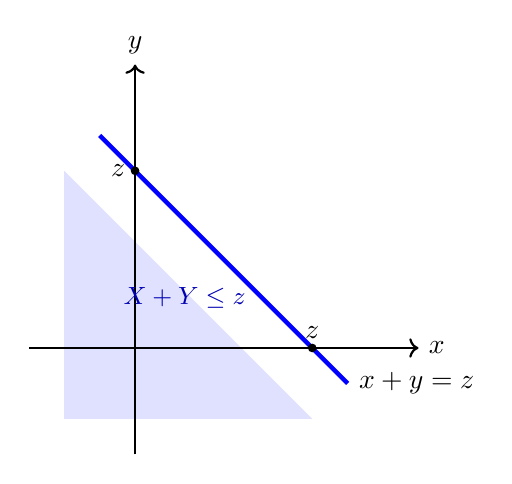
\begin{tikzpicture}[scale=0.9]
    % 1. Define the shaded region FIRST so it stays in the background
    % We use opacity=0.4 to ensure the grid/axes are visible through it
    \fill[blue!20, opacity=0.6] (-1,-1) -- (-1,2.5) -- (2.5,-1) -- cycle;

    % 2. Draw the Axes on top of the shading
    \draw[->, thick] (-1.5,0) -- (4,0) node[right] {$x$};
    \draw[->, thick] (0,-1.5) -- (0,4) node[above] {$y$};
    
    % 3. Draw the Boundary Line x + y = z
    \draw[ultra thick, blue] (-0.5, 3) -- (3, -0.5) node[right, black] {$x + y = z$};
    
    % 4. Add Intercepts and Dots
    \filldraw[black] (0,2.5) circle (1.5pt) node[left] {$z$};
    \filldraw[black] (2.5,0) circle (1.5pt) node[above] {$z$};
    
    % 5. Text Indicators
    \node[blue!70!black, font=\small] at (0.7, 0.7) {$X + Y \leq z$};
\end{tikzpicture}
\caption{Integration region for the sum $Z = X + Y$.}
\end{figure}



\begin{align*}
F_Z(z)  = \iint\limits_{X+Y \leq Z} f_{X,Y}(x,y)dx\, dy
 = \int\limits_Y \int^{z-y}_{-\infty}f_{X,Y}(x,y)\, dx\,dy
 = \int\limits_X \int^{z-x}_{-\infty}f_{X,Y}(x,y)\, dy\,dx.
\end{align*}
Differentiating
\begin{align*}
f_Z(z) &  = \frac{\partial}{\partial z}  \int\limits_Y \int^{z-y}_{-\infty}f_{X,Y}(x,y)\, dx\, dy = \int\limits_Y \left[ \frac{\partial}{\partial z}\int^{z-y}_{-\infty}f_{X,Y}(x,y)\, dx\right]\,dy  = \int\limits_Y f_{X,Y}(z-y,y)\,dy.
\end{align*}
\end{proof}




\item[(b).] If $W = X - Y$, then:
\[f_W(w)   = \int_X f_{X,Y}(x,w+x)\,dx = \int_Y f_{X,Y}(w+y,y)\, dy\, ,\quad Z \in B.\]


\begin{proof}
$F_W(w)  = P(W\leq w) = P(X - Y \leq w)$


\begin{figure}[H]
\centering
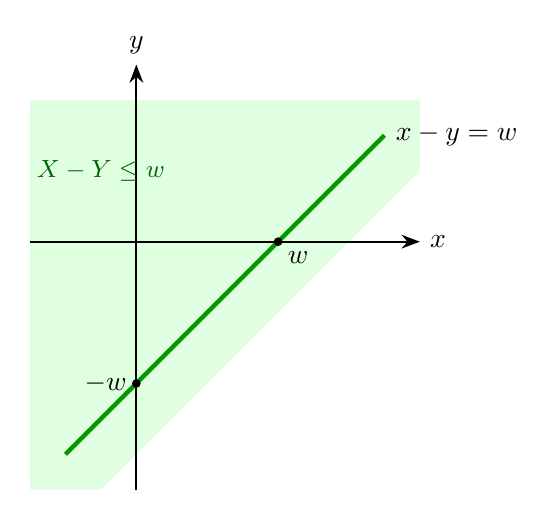
\begin{tikzpicture}[scale=0.9]
    % 1. Shaded Region (X - Y <= w  =>  y >= x - w)
    % We define a large polygon that covers the top-left half-plane
    \fill[green!20, opacity=0.6] (-1.5, 2) -- (4, 2) -- (4, 1) -- (-0.5, -3.5) -- (-1.5, -3.5) -- cycle;
    
    % 2. Axes (Drawn over the fill)
    \draw[-Stealth, thick] (-1.5,0) -- (4,0) node[right] {$x$};
    \draw[-Stealth, thick] (0,-3.5) -- (0,2.5) node[above] {$y$};
    
    % 3. Boundary Line y = x - w
    \draw[ultra thick, green!60!black] (-1, -3) -- (3.5, 1.5) node[right, black] {$x - y = w$};
    
    % 4. Intercepts
    \filldraw[black] (2,0) circle (1.5pt) node[below right] {$w$};
    \filldraw[black] (0,-2) circle (1.5pt) node[left] {$-w$};
    
    % 5. Indicator Text
    \node[green!40!black, font=\small] at (-0.5, 1) {$X - Y \leq w$};
\end{tikzpicture}
\caption{Integration region for the difference $W = X - Y$, with visible axes.}
\end{figure}

\[F_W(w)  =  \iint\limits_{X - Y \leq W} f_{X,Y}(x,y)\, dy\, dx = \int\limits_X\int^{\infty}_{X-W} f_{X,Y}(x,y) \, dy \, dx.\]

Let $y = x- u$\quad $dy = -du$
\begin{figure}[H]
\centering
\begin{tikzpicture}[=>stealth]
\draw[-Stealth](-2,-1)--(-2,0.5);
\draw[-Stealth](2,-1)--(2,0.5);
\draw(-2,0.5)--(-2,1)
(2,0.5)--(2,1);
\draw[->](-0.5,0)--(0.5,0);
\draw(-2,-1)node[right]{$x-w$}
(-2,1)node[right]{$\infty$}
(-2,0)node[left]{$y$}
(2,-1)node[right]{$w$}
(2,1)node[right]{$-\infty$}
(2,0)node[left]{$u$};
\end{tikzpicture}
\end{figure}
\[F_W(w)  = \int\limits_X \int^{-\infty}_{w} (x, x - u)\, (-1)du\, dx = \int\limits_X \int^w_{-\infty} (x, x - u)\, du\, dx\]
Then the PDF
\[f_W(w)  = \frac{\partial}{\partial w}F_W(w)  = \int\limits_X \left( \frac{\partial}{\partial w}\int_{-\infty}^{w} (x, x - u)\, du\right)\, dx = \int\limits_X f_{X,Y}(x,x+w)\, dx.\]
\end{proof}
\end{enumerate}
\end{thm}



\begin{coro}[\textbf{The Convolution Formula}]
If $X$ and $Y$ are independent continuous random variables, the joint PDF factors into $f_X(x)\, f_Y(y)$, then the PDFs  for $Z = X + Y$ and $W = X - Y$ are standard convolution integrals: 
\begin{enumerate}
\item $\displaystyle{f_Z(z) = \int_x f_X(x)f_Y(z-x)dx   =   \int_y f_X(z-y)f_Y(y)dy}$\\

\item $\displaystyle{f_W(w) = \int_x f_X(x)f_Y(x-w)dx   = \int_y f_X(w + y)f_Y(y)dy}$\\
\end{enumerate} 
\end{coro}



\begin{example}
Let $X$ and $Y$ be independent exponential random variables each with mean $\lambda$. Find the distribution of $X+Y$. 
\end{example}

\begin{proof}[\textit{\textbf{Solution}}]
$f_{X,Y}(x,y) = f_X(x)\cdot f_Y(y)$

\[f_X(x) = \frac{1}{\lambda}\, e^{-x/\lambda} \quad \text{and}\quad f_Y(y) = \frac{1}{\lambda}\hspace{0.1cm}e^{-y/\lambda}\] 
Let $Z = X + Y $ , then 

\begin{align*}
f_Z(z)  = \int\limits_x f_X(x) f_Y(z-x)\, dx
& = \int\limits_x \frac{1}{\lambda} e^{-x/\lambda} \cdot \frac{1}{\lambda} e^{-(z-x)/\lambda} dx\\
& = \int\limits_x \frac{1}{\lambda^2} e^{-z/\lambda} dx\\
& = \int^z_0 \frac{1}{\lambda^2} e^{-z/\lambda} dx.\\
& = \frac{z}{\lambda^2} e^{-z/\lambda}\, , \quad z>0,\, \lambda > 0.
\end{align*}

\[f_Z(z) = \frac{z^{2-1}}{\lambda^2}e^{-3/\lambda} \thicksim \operatorname{GAM}(z,\lambda)\]
Thus, $X + Y \thicksim \operatorname{GAM}(z,\lambda)$.
\end{proof}


\begin{note}
Let $X_1, X_2, \cdots, X_k$ be a random sample, if  $X_i \thicksim\operatorname{GAM}(\alpha_i, \lambda)$ then
\[z = \sum^k_{i=1}X_i \thicksim g\left( \sum^n_{i=1} \alpha_i, \lambda\right).\]
\end{note}




\begin{example}
Let $X$ and $Y$ be two independent standard normals, find the distribution of $X-Y$.
\end{example}


\begin{proof}[\textit{Solution}.]
$f_X(x) = \frac{1}{\sqrt{2\pi}}e^{-\frac{1}{2}x^2}$ \quad and  \quad $f_Y(y) = \frac{1}{\sqrt{2\pi}}e^{-\frac{1}{2}y^2}.$

Let $W = X - Y$, then 
\begin{align*}
f_W(w) & = \int^{\infty}_{-\infty} f_X(w+y)f_Y(y) dy\\
& = \int^{\infty}_{-\infty} \frac{1}{\sqrt{2\pi}}\exp\left\{-\frac{1}{2}(w + y)^2\right\}\cdot \frac{1}{\sqrt{2\pi}}\exp\left\{-\frac{1}{2}y^2\right\}\, dy\\
& = \frac{1}{2\pi} \int^{\infty}_{-\infty} \exp\Big\{ -\frac{1}{2}(w^2 + 2yw + 2y^2)\Big\}\, dy\\
& = \frac{\exp\Big\{-\frac{1}{2}w^2\Big\}}{2\pi} \int^{\infty}_{-\infty} \exp\Big\{-\frac{2}{2}\Big(y^2 + yw + \Big(\frac{1}{2}w\Big)^2 - \Big(\frac{1}{2}w\Big)^2\Big)\Big\}\, dy \\
& = \frac{\exp\Big\{-\frac{1}{2}w^2\Big\}}{2\pi} \int^{\infty}_{-\infty} \exp\Big\{-\Big(y + \frac{1}{2}w\Big)^2\Big\}\cdot \exp\Big\{\frac{1}{4}w^2\Big\}\, dy\\
&  = \frac{e^{-\frac{1}{4}w^2}}{\sqrt{2\pi}}\cdot \sqrt{2\pi} \underbrace{\int^{\infty}_{-\infty} \frac{1}{\sqrt{2 \pi\cdot 1/2}}\exp\Big\{-\frac{1}{2}\cdot\frac{(y + \frac{1}{2}w)^2}{1/2}\Big\}\, dy}_1
\end{align*}
Therefore
\[f_W(w) = \frac{e^{-\frac{1}{4}w^2}}{\sqrt{4\pi}}\, ,\quad\quad -\infty < w < \infty\quad  N(0,2)\]
\end{proof}



\begin{exe}
Let $X$ and $Y$ be independent random variables where $X\thicksim \operatorname{GAM}(\alpha_1, \lambda)$ and $Y\thicksim \operatorname{GAM}(\alpha_2, \lambda)$, then $X + Y \thicksim \operatorname{GAM}(\alpha_1 + \alpha_2, \lambda)$.
\end{exe}





\subsection{Distributions of Products and Quotients of Random Variables}
\begin{thm}
Let $X$ and $Y$ be jointly distributed continuous random variables with pdf $f_{X,Y}(x,y)$ and let $Z=\frac{Y}{X}$ and $W = XY$ then 
\begin{enumerate}
\item $\displaystyle{f_Z(z) = \int\limits_X |x|\,f_{X,Y}(x,xz)\,dx}$\\

\item $\displaystyle{f_W(w) = \int\limits_X\frac{1}{|x|}f\left(x,w/x\right)\, dx = \int\limits_Y \frac{1}{|y|}f_{X,Y}\left(w/y,y\right)\, dy}$
\end{enumerate}
\end{thm}


\begin{coro}
Let $X$ and $Y$ be independent continuous random variables, with p.d.f. $f_X(x)$ and $f_Y(y)$, respectively. Assume that $X$ is zero for at most a set of isolated point. Let $Z = \frac{Y}{X}$. Then \[f_Z(z) = \int^{\infty}_{-\infty}|x|\, f_X(x)\,f_Y(zx), dx.\]
\end{coro}

\begin{proof}
\begin{align*}
F_(Z) & = P(Y/X \leq z)\\
& = P(Y/X \leq z\quad \text{and}\quad X\geq 0) + P(Y/X\leq z \quad \text{and}\quad X<0)\\
& = P(Y \leq zX\quad \text{and}\quad X\geq 0) + P(Y\geq zX \quad \text{and}\quad X<0)\\
& = P(Y \leq zX\quad \text{and}\quad X\geq 0) \,+\, 1- P(Y\leq zX \quad \text{and}\quad X<0)\\
& = \int_0^{\infty}\int_{-\infty}^{zx} f_X(x)\, f_Y(y)\, dy dx\, +\, 1 - \int^0_{-\infty}\int_{-\infty}^{zx} f_X(x)f_Y(y)\, dy dx.
\end{align*}
Differentiating $F_Z(z)$ we obtain
\begin{align*}
f_Z(z) & = \frac{d}{dz}F_Z(z)\\
& =\frac{d}{dz}\int_0^{\infty}\int_{-\infty}^{zx}f_X(x) f_Y(y)\, dy dx - \frac{d}{dz}\int_{-\infty}^0\int_{-\infty}^{zx}f_X(x)f_Y(y)\, dy dx\\
& = \int^{\infty}_0f_X(x)\left(\frac{d}{dz}\int_{-\infty}^{zx} f_Y(y)\, dy\right)dx - \int^0_{-\infty}f_X(x)\left(\frac{d}{dz}\int^{zx}_{-\infty} f_Y(y) dy\right)dx
\end{align*}
Note that by the Fundamental Theorem of Calculus and the chain rule, we find
\[\frac{d}{dz}\int_{-\infty}^{zx}f_Y(y)\, dy = f_Y(zx)\, \frac{d}{dz}(zx) = xf_Y(zx).\]
Hence
\begin{align*}
f_Z(z) &  = \int^{\infty}_0xf_X(x)f_Y(zx)\, dx - \int^0_{-\infty}xf_X(x)f_Y(zx)\, dx\\
& = \int^{\infty}_0xf_X(x)f_Y(zx)\, dx + \int^0_{-\infty}(-x)f_X(x)f_Y(zx)\, dx\\
& = \int^{\infty}_0|x|f_X(x)f_Y(zx)\, dx + \int^0_{-\infty}|x|f_X(x) f_Y(zx)\, dx\\
& = \int^{\infty}_{-\infty}|x|\, f_X(x)f_Y(zx)\, dx.
\end{align*}
\end{proof}




\begin{example}
Let $X$ and $Y$ be independent random variables with p.d.fs $f_X(x)  = \lambda e^{-\lambda x}\, ,\, x > 0$, and $f_Y(y) = \lambda e^{-\lambda y}\,,\, y > 0$, respectively. Define $Z = Y/X$. Find $f_Z(z)$.
\end{example}
\begin{proof}[\textbf{\textit{Solution}}]
We can write
\begin{align*}
f_Z(z) & = \int^{\infty}_0x(\lambda e^{-\lambda zx}(\lambda e^{-\lambda zx})\, dx\\
& = \lambda^2\int^{\infty}_0xe^{-\lambda(1 + z)x}\, dx\\
& = \frac{\lambda^2}{\lambda (1 + z)}\int^{\infty}_0x\lambda(1 + z)e^{-\lambda (1 + z)x}\, dx\\
& = \frac{\lambda^2}{\lambda (1 + z)}\cdot\frac{1}{\lambda(1+z)}\int^{\infty}_0t e^{-t}\, dt,\quad\quad \text{letting} \,\, t = x\lambda (1 + z)\\ 
& = \frac{\lambda^2}{\lambda^2 (1 + z)^2}\, 1!\\
& = \frac{1}{(1+z)^2}\, , \quad z\geq 0
\end{align*}
\end{proof}








\begin{thm}
If $X$ and $Y$ are discrete random variables having joint distribution function $f_{X,Y}(x,y)$.
Let $Z = X + Y $ and $ W = X - Y$, then 
\begin{align*}
f_Z(z)  = P(Z= z) & = \sum_X f_{X,Y} (x,z -x)\\
& = \sum_X P(X = x, Y = z -x)\\
& = \sum_Y f_{X,Y} (z-y,y)\\
& = \sum_Y P(X = z - y, Y =y).
\end{align*}
and
\begin{align*}
f_W(w)  = P(W = w) & = \sum_X f_{X,Y} (x, x - w)\\
& = \sum_Y f_{X,Y} (w +y,y).
\end{align*}
\end{thm}







\begin{example}
The joint probability function of $X$ and $Y$ is given in the table below\\

\begin{table}[H]
\centering
$Y$\\
\begin{tabular}{c|cccc|c}
$X$ & 1 & 2 & 3 & 4 & $f_X(x)$\\
\hline
&&&&&\\
1 & 0.10 & 0.05 & 0.02 & 0.02 & 0.19\\
&&&&&\\
2 & 0.05 & 0.20 & 0.05 & 0.20 & 0.5\\
&&&&&\\
3 & 0.02 & 0.05 & 0.02 & 0.04 & 0.13\\
&&&&&\\
4 & 0.02 & 0.02 & 0.04 & 0.10 & 0.18\\
&&&&&\\
\hline
&&&&&\\
$f_Y(y)$ & 0.19 & 0.32 & 0.13 & 0.36 & \\
\end{tabular}
\end{table}
Find the distribution of $Z = X + Y $ and $W = X - Y$.
\end{example}


\begin{proof}[\textbf{\textit{Solution}}]
The distribution for $Z$ is 
\begin{table}[H]
\centering
\begin{tabular}{|c|ccccccc|}
\hline
$Z$ & 2 & 3 & 4 & 5 & 6 & 7 & 8\\
\hline
&&&&&&&\\
$f_Z(z)$ & 0.10 & 0.10 & 0.24 & 0.14 & 0.24 & 0.08 & 0.10\\
\hline
\end{tabular}
\end{table}

and for $W$ is
\begin{table}[H]
\centering
\begin{tabular}{|c|ccccccc|}
\hline
$W$ & $-3$ & $-2$ & $-1$ & 0 & 1 & 2 & 3 \\
\hline
&&&&&&&\\
$f_W(w)$ & 0.02 & 0.22 & 0.14 & 0.42 & 0.14 & 0.04 & 0.02\\
\hline
\end{tabular}
\end{table}
\end{proof}



\subsection{Moment Generating Function Method}
\vspace{-15pt}
The power of the MGF method lies in the property that the MGF of a sum of independent variables is the product of their individual MGFs.

\begin{thm}
If $X_1, X_2, \cdots, X_n$ are independent random variables with MGFs $M_{X_i}(t)$ then the MGF of $Y = \sum^n_{i = 1}X_i$ is \[M_{Y}(t) = M_{X_1}(t)\, M_{X_2}(t)\, \cdots\, M_{X_n}(t).\]
\end{thm}
\begin{proof}
\begin{align*}
M_Y(t) & = E(e^{tY})\\
& = E\left(e^{t(X_1 + X_2 + \cdots + X_n)}\right)\\
& = E\left(e^{tX_1 + tX_2 + \cdots + tX_n}\right)\\
& = E\left(e^{tX_1}\right) E\left(e^{tX_2}\right)  \cdots  E\left(e^{tX_n}\right)\quad\quad \text{since the}\,\,\, X_i's\,\,\, \text{are independent}\\
& = M_{X_1}(t)\, M_{X_2}(t)\, \cdots \, M_{X_n}(t)
\end{align*}
\end{proof}



\begin{note}
If $X_1, X_2, \cdots , X_n$ are i.i.d. random variables each with MGF. $M_X(t)$, then the MGF of $Y$ is \[M_Y(t)  = \left[M_X(t)\right]^n.\]
\end{note}



\subsubsection{Special Results:}
These results are frequently used in sampling theory and are derived directly from the MGF properties:
\begin{enumerate}
\item If $X\thicksim \operatorname{GAM}(\alpha,\beta)$, where $\alpha$ is positive, then \[\frac{2X}{\beta} \thicksim \chi^2(2\alpha).\]
\item If $X_i \thicksim \operatorname{GAM}(\alpha_i,\beta)$, \, $i = 1, 2, \cdots, n$ independently then \[\sum^n_{i = 1} X_i \thicksim\operatorname{GAM}\left(\sum^n_{i = 1} \alpha_i, \beta\right).\]
\item If $X_i \thicksim \operatorname{GAM}(1,\beta) = \operatorname{EXP}(\beta)$, \, $i  = 1, 2, \cdots , n$ independently, then \[\sum^n_{i = 1}X_i \thicksim \operatorname{GAM}(n,\beta).\]
\item If $X_i \thicksim \operatorname{N}(\mu,\sigma^2)$, \, $i = 1, 2, \cdots , n$ independently, then \[\sum^n_{i = 1}\left(\frac{X_i - \mu}{\sigma}\right)^2\,\thicksim\, \chi^2_{(n)}.\]
\end{enumerate}



\begin{example}
Let $X_1, X_2, \, \cdots, \, X_n$ be independent Poisson-distributed random variables, $X_i \thicksim \operatorname{POI}(\mu_i)$. Show that \[Y = \sum^n_{i = 1} X_i \, \thicksim\, \operatorname{POI}\left(\sum^n_{i = 1} \mu_i\right).\]
\end{example}


\begin{proof}[\textit{Solution}.]
\[f_{X_i}(x_i) = \frac{e^{-\mu_i}\, \mu_i^{x_i}}{x_i!}\, , \quad x_i = 0, 1, 2, \cdots\]
Recall that $$M_{X_i}(t)  = e^{\mu_i(e^t - 1)}$$
now
\begin{align*}
M_Y(t) & = \prod^n_{i =1} M_{X_i}(t)\\
& = \prod^n_{i =1} e^{\mu_i(e^t-1)}\\
& = e^{\left(\sum^n_{i =1}\mu_i\right)(e^t - 1)}
\end{align*}
Therefore, $\, Y \thicksim \operatorname{POI}\left(\sum^n_{i = 1}\mu_i\right)$.
\end{proof}



\begin{exe}
\begin{enumerate}
\item Let $X_1, X_2, \cdots , X_n$ be independent binomial random variables, $X_i\thicksim \operatorname{BIN}(n_i,p)$. Show that \[Y = \sum^n_{i =  1}X_i \thicksim \operatorname{BIN}\left(\sum^n_{i = 1}n_i,p\right).\]
\item If $X_1, X_2, \cdots, X_n$ are independent negative binomial random variables, $X_i \thicksim \operatorname{NB}(k_i,p)$, show that \[Y = \sum^n_{i = 1} X_i \thicksim \operatorname{NB}\left(\sum^n_{i = 1}k_i,p\right).\]
\end{enumerate}
\end{exe}



\begin{thm}
Let $X_1, X_2, \cdots , X_n$ be independent normally distributed random variables, $X_i \thicksim \operatorname{N}(\mu_i,\sigma_i^2)$, then \[\sum^n_{i = 1}a_iX_i \, \thicksim\, \operatorname{N}\left(\sum^n_{i = 1} a_i\mu_i, \sum^n_{i = 1}a_i^2\sigma^2_i\right).\]
\end{thm}

\begin{proof}
Recall \[M_{X_i}(t) = e^{\mu_i t + \frac{1}{2}\sigma^2_it^2}\]
Let $Y = \sum^n_{i = 1} a_i X_i$
\begin{align*}
M_Y(t) & = E\left(e^{tY}\right)\\
& = E\left(e^{t\sum^n_{i = 1}a_iX_i}\right)\\
& = \prod^n_{i = 1}E\left(e^{ta_iX_i}\right)\\
& = \prod^n_{i = 1}e^{\mu_ia_it + \frac{1}{2}\sigma^2_ia^2_it^2}\\
& = e^{\left(\sum^n_{i =1}\mu_ia_i\right)t + \frac{1}{2}\left(\sum^n_{i = 1}\sigma^2_ia^2_i\right)t^2}
\end{align*}
Therefore \[Y = \sum^n_{i = 1} a_iX_i \, \thicksim\, \operatorname{N}\left(\sum^n_{i = 1}a_i \mu_i\, , \, \sum^n_{i = 1} a_i^2\sigma^2_i\right).\]
\end{proof}





\begin{coro}
If $X_i\overset{iid}{\thicksim}\operatorname{N}(\mu,\sigma^2)$, then \[\sum^n_{i = 1} X_i \thicksim \operatorname{N}(n\mu, n\sigma^2)\] and \[\overline{X} = \frac{1}{n}\sum^n_{i = 1}X_i \thicksim \operatorname{N}(\mu, \frac{\sigma^2}{n}).\]
\end{coro}

\begin{proof}
$M_{X_i}(t) = e^{\mu t + \frac{1}{2}\sigma^2 t^2}$

Let $\, Y = \sum^n_{i = 1} X_i$
\begin{align*}
M_Y(t) & = E(e^{tY})\\
& = E\left(e^{t\sum^n_{i = 1} X_i}\right)\\
& = \left[M_X(t)\right]^n\\
& = \left(e^{\mu t + \frac{1}{2}\sigma^2 t^2}\right)^n\\
& = e^{n\mu t + \frac{1}{2}n\sigma^2t^2}.
\end{align*}

Therefore \[Y = \sum^n_{i = 1}X_i \thicksim\operatorname{N}(n\mu, n\sigma^2)).\]
\end{proof}




\begin{thm}
If $\, X \thicksim \chi^2(n)$ then \[f(x) = \frac{1}{2^{\frac{n}{2}}\Gamma\left(\frac{n}{2}\right)}\, x^{\frac{n}{2}-1}\, e^{-\frac{x}{2}}\, , \quad x > 0\] and \[M_X(t) = \left(\frac{1}{1-2t}\right)^{\frac{n}{2}}\,, \quad E(X) = n\, , \quad \operatorname{Var}(X) = 2n.\]
\end{thm}

\begin{proof}
\begin{align*}
M_X(t) & = E\left(e^{tX}\right)\\
& = \int^{\infty}_0e^{tx}\, \frac{x^{\frac{n}{2-1}}\, e^{-\frac{x}{2}}}{2^{\frac{n}{2}}\, \Gamma\left(\frac{n}{2}\right)}\, dx\\
& = \frac{1}{2^{\frac{n}{2}}\, \Gamma\left(\frac{n}{2}\right)}\,\int_0^{\infty}x^{\frac{n}{2}-1}\, e^{-(\frac{1}{2}-t)x}\, dx\\
& = \frac{1}{2^{\frac{n}{2}}\, \Gamma\left(\frac{n}{2}\right)}\,\int_0^{\infty}\left(\frac{y}{\frac{1}{2}-t}\right)^{\frac{n}{2}-1}\, e^{-y}\, \frac{dy}{\frac{1}{2}-t}\, ,\quad \text{letting}\,\, y = (\frac{1}{2}-t)x\\
& = \frac{1}{2^{\frac{n}{2}}\Gamma\left(\frac{n}{2}\right)}\, \frac{1}{\left(\frac{1}{2}-t\right)^{\frac{n}{2}}}\int_0^{\infty} y^{\frac{n}{2}-1}\, e^{-y}\, dy \, , \quad t > \frac{1}{2}\\
& = \frac{\Gamma\left(\frac{n}{2}\right)}{\Gamma\left(\frac{n}{2}\right) (1-2t)^{\frac{n}{2}}}\\
& = \left(\frac{1}{1-2t}\right)^{\frac{n}{2}}\, , \quad\quad t > \frac{1}{2}.
\end{align*}

\[M'_X(t) = -\frac{n}{2}(1 - 2t)^{-\frac{n}{2}-1}(-2) = n(1 - 2t)^{-\frac{n}{2}-1}.\]

\[M''_X(t) = n\left(-\frac{n}{2}-1\right)(1-2t)^{-\frac{n}{2}-2}(-2) = 2n\left(\frac{n}{2} + 1\right)(1 - 2t)^{-\frac{n}{2}-2}.\]

\[E(X) = M'_X(0) = n.\]

\[E(X^2) = M''_X(0) = 2n\left(\frac{n}{2} + 1\right).\]

\[\operatorname{Var}(X) = 2n\left(\frac{n}{2}+1\right) - n^2 = n^2 + 2n -n^2 = 2n.\]
\end{proof}
%%%%%%%%%%%%%%%%%%%%%%%%%%%%%%%%%%%%%%%%%%%%%%%%%%%%%%%%%%%%%%%%%%%%




\subsection{Distribution of $t$,$\chi^2$ and $F$ Random Variables}

\begin{definition}[\textbf{Chi-squared distribution $\chi^2$}]
A random variable $X$ with the following pdf is known as a chi-squared with $k$ degrees of freedom \[f_X(x) = \frac{x^{\frac{k}{2}-1}e^{-\frac{x}{2}}}{\Gamma\left(\frac{k}{2}\right)\, 2^{\frac{k}{2}}}\,\, , \quad x>0.\]
\end{definition}




\begin{remark}
\textbf{ }
\begin{enumerate}
\item If $Y \thicksim \operatorname{GAM}( \alpha, \lambda )$ , then \[f_Y(y) = \frac{y^{\alpha -1} \lambda^{\alpha} e^{-\lambda y}}{\Gamma (\alpha)} \, , \quad y>0\]
Therefore a chi-square with $k$ degrees of freedom is a gamma with $\alpha = \frac{k}{2}$ and $\lambda = \frac{1}{2}$.

\item $E(Y) = \frac{\alpha}{\lambda}$ and $\operatorname{Var}(Y) = \frac{\alpha}{\lambda^2}$. Therefore $E(X) = \frac{k/2}{1/2} = k$ and  $\operatorname{Var}(X) = \frac{k/2}{(1/2)^2} = 2k$.

\item Thus the mean of a chi-square is equal to its degrees of freedom while the variance is twice its degrees of freedom.\\

\item $M_Y(t) = \left( \frac{\lambda}{\lambda - t}\right)^{\alpha}$

Therefore
\[M_X(t) = \left(\frac{\frac{1}{2}}{\frac{1}{2}-t}\right)^{\frac{k}{2}} = \left(\frac{1}{1-2t}\right)^{\frac{k}{2}} = \left(\frac{1}{\sqrt{1 - 2t}}\right)^k.\]
\end{enumerate}
\end{remark}





\begin{thm}
If the random variables $X_1, X_2, \cdots, X_k$ are independent and normally distributed with $X_j$ having mean $\mu_j$ and variance $\sigma_j^2$ i.e $X_j'$s and  $N(\mu_j, \sigma^2_j)$ then \[W = \sum^k_{j=1}\left(\frac{X_j - \mu_j}{\sigma_j}\right)^2\] has a chi-square distribution with $k$ degrees of freedom.
\end{thm}





\begin{remark}
If $Z_j = \frac{X_j - \mu_j}{\sigma_j}$ then $Z_j \thicksim N(0,1), \quad j = 0, 1, 2, \cdots, k$ then $Z_j$ is standard normal. Therefore chi-square is a sum of squares of  independent standard normals.
\end{remark}


\begin{proof}
We find the m.g.f of $W$
\begin{align*}
M_W(t)  = E\left(e^{tw}\right) & = E\left( e^{t\sum^k_{j=1}\left(\frac{X_j-\mu_j}{\sigma_j}\right)^2}\right)\\
& = E\left( e^{\sum\limits^k_{j=1} Z_j^2t}\right)\,\,\quad \text{where}\quad Z_j= \frac{X_j - \mu_j}{\sigma_j}\\
& = E\left( \prod^k_{j=1} e^{tZ^2_j}\right)\\
& = \prod^k_{j=1} E\left(e^{tZ^2_j}\right)\\
& = \left[E\left(e^{tZ^2}\right)\right]^k\quad , \quad Z \thicksim N(0,1)
\end{align*}
now find
\begin{align*}
E\left(e^{tz^2}\right) & = \int^{\infty}_{-\infty} e^{tZ^2}\, f_Z(z)\, dz\\
& = \int^{\infty}_{-\infty} e^{tz^2}\, \frac{1}{\sqrt{2\pi}}e^{-\frac{1}{2}z^2}\,dz\\
& = \int^{\infty}_{-\infty} \frac{1}{\sqrt{2 \pi}}e^{-\frac{1}{2}(1 - 2t)z^2}\, dz\\
 & = \int^{\infty}_{-\infty} \frac{1}{\sqrt{2\pi}}e^{-\frac{1}{2} u^2} \, \frac{du}{\sqrt{1 - 2t}}\, ,\quad \quad \text{letting}\,\, u = \sqrt{1 - 2t}\,z\\
& = \frac{1}{\sqrt{1 - 2t}}\underbrace{\int^{\infty}_{-\infty} \frac{1}{\sqrt{2\pi}}e^{-\frac{1}{2} u^2} \, du}_1\\
& = \frac{1}{\sqrt{1 - 2t}}.
\end{align*}
Therefore,
$$M_w(t) = \left[E\left(e^{tz^2}\right)\right]^k = \left[ \frac{1}{\sqrt{1 - 2t}}\right]^k$$
By uniqueness theorem of m.g.f. $W$ has a chi-square distribution with $k$ degrees of freedom.
\end{proof}









\begin{coro}
If $X_1, X_2,\cdots, X_n$ is a random sample from $N\thicksim (\mu, \sigma^2)$ then \[M = \sum^n_{j=1} \left( \frac{X_j - \mu}{\sigma}\right)^2 \thicksim \chi^2_n.\]
\end{coro}




\begin{definition}[\textbf{$F$-Distribution}]
If a random variable $X$ has the following p.d.f. \[f_X(x) = \frac{\Gamma \left(\frac{m + n}{2}\right)\, \left(\frac{m}{n}\right)^{\frac{m}{2}}\, x^{\frac{m}{2}-1}}{\Gamma\left(\frac{m}{2}\right)\,\Gamma \left(\frac{n}{2}\right)\, \left(1 + \frac{m}{n}x\right)^{\frac{m+n}{2}}}\, , \quad x>0\]
then $X$ has an $F -$ distribution with $m$ degrees of freedom in the numerator and $n$ degrees of freedom in the denominator.
\end{definition}

\begin{thm}
If $U$ and $V$ are independent chi-square random variables with $m$ and $n$ degrees of freedom respectively then $X = \frac{U/m}{V/n}$ has $F -$ distribution with $m$ degrees of freedom in the numerator and $n$ degrees of freedom in the denominator.
\end{thm}




\begin{remark}
The $F - $ distribution is the ratio of two independent Chi - squares divided by their respective degrees of freedom.\\
\end{remark}






To prove the theorem we will follow the steps:
\begin{enumerate}
\item[ ]\textbf{\textit{Step I:}} Find the joint p.d.f. of $U$ and $V$.

\item[ ]\textbf{\textit{Step II:}} Make a transformation $$(U,V) \hspace{0.5cm} \longrightarrow \hspace{0.5cm} (X,Z)$$
where $X = \frac{U/m}{V/n}\hspace{0.5cm} , \hspace{0.5cm} Z = V$.\\

Find the Jacobian of transformation.

\item[ ]\textbf{\textit{Step III:}} Find the joint p.d.f. of $X$ and $Z$.

\item[ ]\textbf{\textit{Step IV:}} Find the marginal p.d.f. of $X$.
\end{enumerate}





\begin{proof}
We find the joint p.d.f of $U$ and $V$
\begin{align*}
f_{U,V}(u,v) &  = f_U(u) \cdot f_V(v)\\
& = \frac{u^{\frac{m}{2}-1}\, e^{-\frac{u}{2}}}{\Gamma\left(\frac{m}{2}\right)\, 2^{\frac{m}{2}}}\cdot \frac{v^{\frac{n}{2}-1}\, e^{-\frac{v}{2}}}{\Gamma\left(\frac{n}{2}\right)\, 2^{\frac{n}{2}}}\\
& = \frac{u^{\frac{m}{2}-1}v^{\frac{n}{2}-1} e^{\frac{-(u+v)}{2}}}                                                               {2^{\frac{m + n}{2}}\, \Gamma \left(\frac{m}{2}\right) \, \Gamma\left(\frac{n}{2}\right)}.
\end{align*}


We make  a transformation,
\[X = \frac{U/m}{V/n} \quad \text{and} \quad Z = V\]  

\[X = \frac{U/m}{Z/n} \quad\implies\quad \frac{ZX}{n} = \frac{u}{m}\]


\[\implies \quad U = \frac{m}{n}ZX\quad ;\quad V = Z\]
and the Jacobian
\[J  = \begin{vmatrix}
\frac{\partial U}{\partial x} & \frac{\partial U}{\partial z}\\
\frac{\partial V}{\partial x} & \frac{\partial V}{\partial z}\\
\end{vmatrix} = \begin{vmatrix}
\frac{m}{n}z & \frac{m}{n}x\\
0 & 1\\
\end{vmatrix}
 = \frac{m}{n}z.\]


We find the joint p.d.f of $X$ and $Z$
\begin{align*}
f_{X,Z}(x,z) & = f_{U,V}(x,z)\, |J|\\
&  = \frac{\left(\frac{m}{n}zx\right)^{\frac{m}{2}-1}\, z^{\frac{n}{2}-1}\, e^{-\frac{z}{2}\left(1 + \frac{m}{n}x\right)}}{2^{\frac{m+n}{2}}\, \Gamma \left(\frac{m}{2}\right)\,\Gamma \left(\frac{n}{2}\right)}\,\begin{vmatrix}
\frac{m}{n}z\\
\end{vmatrix}\\
& = \frac{\left(\frac{m}{n}\right)^{\frac{m}{2}}z^{\frac{m+n}{2}-1}\, x^{\frac{m}{2}-1}\, e^{-\frac{z}{2}\left(1 + \frac{m}{n}x\right)}}{2^{\frac{m+n}{2}}\, \Gamma \left(\frac{m}{2}\right)\,\Gamma \left( \frac{n}{2}\right)}\quad ,\quad\quad x>0\, , \, z>0.
\end{align*}


Now we find the marginal p.d.f of $X$
\begin{align*}
f_X(x) & = \int\limits_Z f_{X,Z}(x,z)\, dz\\
& = \frac{\left(\frac{m}{n}\right)^{\frac{m}{2}}\, x^{\frac{m}{2}-1}}{2^{\frac{m+n}{2}}\, \Gamma \left(\frac{m}{2}\right)\, \Gamma \left(\frac{n}{2}\right)}\int^{\infty}_0 z^{\frac{m+n}{2}-1}\, e^{-\frac{z}{2}\left(1 + \frac{m}{n}x\right)}\, dz.
\end{align*}

Let\, $y = \frac{z}{2}\left(1 + \frac{m}{n}x\right)$ \[\implies\quad dy = \frac{1}{2}\left(1 + \frac{m}{n}x\right)\, dz\]
\[dz = \frac{2}{\left(1 + \frac{m}{n}x\right)}\, dy\]
now replacing 
\begin{align*}
f_X(x) & = \frac{\left(\frac{m}{n}\right)^{\frac{m}{2}}\, x^{\frac{m}{2}-1}}{2^{\frac{m+n}{2}}\, \Gamma \left(\frac{m}{2}\right)\,\Gamma \left(\frac{n}{2}\right)}\int^{\infty}_0 \left(\frac{2y}{1 + \frac{mx}{n}}\right)^{\frac{m+n}{2}-1}\, e^{-y}\, \left(\frac{2}{1 + \frac{m}{n}x}\right)\, dy\\
& = \frac{\left(\frac{m}{n}\right)^{\frac{m}{2}}\, x^{\frac{m}{2}-1}\, 2^{\frac{m+n}{2}}}{2^{\frac{m+n}{2}}\,  \Gamma \left(\frac{m}{2}\right)\,\Gamma \left(\frac{n}{2}\right)\, \left(1 + \frac{m}{n}x\right)^{\frac{m + n}{2}}} \int^{\infty}_0 y^{\frac{m+n}{2}-1}\,  e^{-y} \, dy\\
& =\frac{\left(\frac{m}{n}\right)^{\frac{m}{2}}\, x^{\frac{m}{2}-1}\,\Gamma\left(\frac{m + n}{2}\right)}{\Gamma \left(\frac{m}{2}\right)\,\Gamma \left(\frac{n}{2}\right)\, \left(1 + \frac{m}{n}x\right)^{\frac{m + n}{2}}}.
\end{align*}
\end{proof}














\begin{definition}[\textbf{$t$ Distribution}]
Let $Z$ be a standard normal random variable and $U$ be chi-square random variable with $m$ degrees of freedom. If $Z$ and $U$ are independent then the distribution of \[ Y = \frac{Z}{\sqrt{\frac{U}{m}}}\] is called the $t -$ distribution with $m$ degrees of freedom.
\end{definition}




\begin{remark}
\[T = \frac{\left(\overline{X} - \mu\right)}{S}\sqrt{n} = \frac{\frac{\left(\overline{X}-\mu\right)}{\sigma / \sqrt{n}}}{\sqrt{\frac{(n-1)\, S^2}{\sigma^2/(n-1)}}} = \frac{N(0,1)}{\sqrt{\frac{\chi^2_{n-1}}{n-1}}}.\]
\end{remark}



\begin{thm}
The p.d.f. of a random variable $Y$ with $t -$ distribution with $m$ degrees of freedom given by \[f_Y(y) = \frac{\Gamma \left(\frac{m + 1}{2}\right)}{\sqrt{m\pi}\, \Gamma\left(\frac{m}{2}\right)\,\left(1 + \frac{y^2}{m}\right)^{\frac{m+1}{2}}}\, , \quad y \in (-\infty, \infty).\]
\end{thm}



\begin{note}
To prove the theorem we
\begin{enumerate}
\item[ ]\textbf{\textit{Step I:}} Find the joint pdf of $Z$ and $U$.

\item[ ]\textbf{\textit{Step II:}} Make a transformation $$(Z,U) \longrightarrow (X,Y)\hspace{0.2cm} , \hspace{0.2cm} X = U \hspace{0.3cm}\text{and}\hspace{0.3cm} Y = \frac{Z}{\sqrt{\frac{U}{m}}}$$ Find the Jacobian of transformation.

\item[ ]\textbf{\textit{Step III:}} Find the Joint pdf of $X$ and $Y$.

\item[ ]\textbf{\textit{Step IV:}} Find the marginal of $Y$.
\end{enumerate}
\end{note}




\begin{proof}
Let $Z \thicksim N(0,1)$ and $U\thicksim \chi^2_m$ with $Z$ and $U$ being independent.

We first find the joint p.d.f. of $Z$ and $U$
\begin{align*}
f_{Z,U} (z,u) & = f_Z(z)\, f_U(u)\\
& = \frac{1}{\sqrt{2\pi}}e^{-\frac{1}{2}z^2}\, \frac{u^{\frac{m}{2}} e^{-\frac{u}{2}}}{\Gamma \left(\frac{m}{2}\right)\, 2^{\frac{m}{2}}}\\
 & = \frac{u^{\frac{m}{2}-1}\, e^{-\frac{1}{2}(u + z^2)}}{\sqrt{2\pi}\, 2^{\frac{m}{2}}\, \Gamma \left(\frac{m}{2}\right)}\, ,\quad z \in (-\infty, \infty)\, , \quad u\in (0,\infty).
\end{align*}
Make a transformation
\[X = U\quad \text{and}\quad Y = \frac{Z}{\sqrt{\frac{U}{m}}}\quad \implies \quad U = x\, , \quad Z = Y\sqrt{\frac{X}{m}}.\]
The Jacobian
\[J  = \begin{vmatrix}
\frac{\partial U}{\partial x} & \frac{\partial U}{\partial y}\\
\frac{\partial Z}{\partial x} & \frac{\partial Z}{\partial y}\\
\end{vmatrix} = 
\begin{vmatrix}
1 & 0 \\
? & \sqrt{\frac{x}{m}}\
\end{vmatrix} = \sqrt{\frac{x}{m}}.\]

Then the joint p.d.f. of $X$ and $Y$
\[f_{X,Y}(x,y) = \frac{x^{\frac{m}{2}-1}\, e^{-\frac{1}{2}\left(x + y^2 \frac{x}{m}\right)}}{\sqrt{2\pi}\, 2^{\frac{m}{2}}\, \Gamma \left(\frac{m}{2}\right)} \, \sqrt{\frac{x}{m}}\,  ,\quad x>0\, , \quad y \in (-\infty, \infty).\]

We now find the marginal of $Y$
\[f_Y(y)  = \int\limits_X f_{X,Y}(x,y)\, dy\\
 = \frac{1}{\sqrt{2\pi}\, 2^{\frac{m}{2}}\, \Gamma \left(\frac{m}{2}\right)\, \sqrt{m}}\int^{\infty}_0 x^{\frac{m-1}{2}}\, e^{-\frac{1}{2}\left(x + y^2 \frac{x}{m}\right)}\, dx.\]


Let $\, V = \frac{1}{2}\left(1 + \frac{y^2}{m}\right)\quad x \implies\quad dV = \frac{1}{2}\left(1 + \frac{y^2}{m}\right)\, dx$

\[dx = \frac{2 dv}{\left(1 + \frac{y^2}{m}\right)}\quad , \quad X = \frac{2 v}{1 + \frac{y^2}{m}}.\]
Thus
\begin{align*}
f_Y(y) & =  \frac{1}{\sqrt{2\pi}\, 2^{\frac{m}{2}}\, \Gamma \left(\frac{m}{2}\right)\, \sqrt{m}} \int^{\infty}_0 \left(\frac{2 v}{1 +\frac{y^2}{m}}\right)^{\frac{m - 1}{2}}\, e^{-v}\, \frac{2dv}{\left(1 + \frac{y^2}{m}\right)}\\
& = \frac{2^{\frac{m+1}{2}}}{\sqrt{2\pi}\, 2^{\frac{m}{2}}\, \Gamma \left(\frac{m}{2}\right)\, \sqrt{m}\, \left( 1 + \frac{y^2}{m}\right)^{\frac{m+1}{2}}}\, \underbrace{\int^{\infty}_0 v^{\frac{m - 1}{2}}\, e^{-1}\, dv}_{\Gamma \left(\frac{m+1}{2}\right)}\\
& = \frac{\Gamma \left(\frac{m + 1}{2}\right)}{\sqrt{\pi}\, \Gamma \left(\frac{m}{2}\right)\, \left(1 + \frac{y^2}{m}\right)^{\frac{m+1}{2}}\, \sqrt{m}}\\
& = \frac{\Gamma \left(\frac{m + 1}{2}\right)}{\sqrt{m \pi}\, \Gamma \left(\frac{m}{2}\right)\, \left(1 + \frac{y^2}{m}\right)^{\frac{m+1}{2}}}\, ,\quad y \in (-\infty, \infty).
\end{align*}
\end{proof}





























%%%%%%%%%%%%%%%%%%%%%%%%%%%%%%%%%%%%%%%%%%%%


















% Estimation
%%%%%%%%%%%%%%%%%%%%%%%%%%%%%%%%%%%%%%%%%%%%%%%%%%%%%
\chapter{Estimation}

\section{Introduction}
\vspace{-15pt}
In statistical inference, we assume our data $X_1, X_2, \dots, X_n$ comes from a distribution $f(x; \theta)$, but the true value of $\theta$ is hidden from us. Our goal is to use the sample to construct a ``best guess" for the unknown parameter $\theta \in \Omega$, where $\Omega$ represents the parameter space.



\begin{definition}
A statistic $T = T(X_1, X_2,  \cdots , X_n)$, if a function of the data which does not depend on the unknown parameter $\theta$.
\end{definition}



\begin{example}
The sample mean $\bar{X} = \frac{1}{n}\sum X_i$ is a statistic. While, the quantity $\frac{\bar{X} - \mu}{\sigma / \sqrt{n}}$ is not a statistic if $\mu$ or $\sigma$ are unknown.
\end{example}



\begin{definition}
An Estimator is a statistic used to approximate an unknown parameter. It is a random variable denoted by $\hat{\theta}$.
\end{definition}

\begin{definition}
An Estimate is the specific numerical value of the estimator obtained from a realized data set $(x_1, x_2, \dots, x_n)$.
\end{definition}



\begin{definition}
Let $X_1, X_2, \cdots , X_n$ be a random sample from a population (with a population distribution), then 
\begin{enumerate}
\item[(a).] the $k^{\text{th}}$ sample moment about 0 is given by \[M_k' = \frac{1}{n}\sum^n_{i =1}X^k_i\]
\item[(b).] the $k^{\text{th}}$ sample moment about the mean $\overline{X}$ is given by \[M_k = \frac{1}{n}\sum^n_{i = 1}(X_i - \overline{X})^k.\]
\end{enumerate}
\end{definition}




\begin{note}\textbf{ }
\begin{enumerate}
\item 
\begin{enumerate}
\item $\mu'_k = E(X^k)$ is the $k^{\text{th}}$ (population) moment at 0.
\item $\mu_k = E(X - \mu)^k$ is the $k^{\text{th}}$ (population) moment about the mean $\mu$.
\end{enumerate}
\item $M'_1 = \frac{1}{n}\sum^n_{i = 1}X_i = \overline{X}, \quad M_1 = 0$
\end{enumerate}
\end{note}



\begin{thm}
Let $X_1, X_2, \cdots, X_n$ be a random sample from a population (with a population distribution), then \[E(M'_k) = \mu'_k \quad\quad (\text{if}\quad \mu'_k\quad \text{exists})\]
\[\operatorname{Var}(M_k') = \frac{1}{n}\left(\mu'_{2k} - (\mu'_k)^2\right) \quad (\text{if}\quad \mu'_{2k}\quad \text{exist})\]
\end{thm}

i.e. if $k = 1$, then 
\[E(\overline{X})  = \mu_1' = E(X) = \mu\]
\begin{align*}
\operatorname{Var}(\overline{X}) & = \frac{1}{n}\left[\mu_2' - (\mu_1')^2 \right]\\
& = \frac{1}{n}\left[E(X^2) - (E(X))^2\right]\\
& = \frac{1}{n}\, \operatorname{Var}(X)\\
& = \frac{\sigma^2}{n}.
\end{align*}




\begin{definition}
A statistic $T = T(X_1,X_2, \cdots , X_n)$ that is used to estimate $\theta$ or $\tau(\theta)$, a function of $\theta$, is called an estimator of $\tau(\theta)$ and an observed value of the statistic $t = t(x_1, x_2, \cdots , x_n)$ is called an estimate of $\tau(\theta)$.
\end{definition}


\begin{example}
If $X_1, X_2, \cdots , X_n$ are i.i.d random variables with $E(X_i) = \mu$ then $\overline{X}$ is an estimator of $\mu$ and $\overline{x}$ is an estimate of $\mu$.
\end{example}



There are a number of methods of finding estimators of $\theta$ or $\tau(\theta)$, some of them include: 
\begin{enumerate}
\item method of moments (MME)
\item maximum likelihood method (MLE)
\item least squares method (mainly in regression) (LSE)
\end{enumerate}






\section{Method of Moments}
Consider a population PDF, $f(x;\theta_1, \theta_2, \cdots , \theta_k)$, depending on one or more parameters $\theta_1, \theta_2, \cdots , \theta_k$.

Method of moments estimators are solutions to the following system of equations \[M'_j=\mu'_j,\quad j=1,2,\cdots,k\]

\begin{example}
Find the method of moments estimators for $\mu$ and $\sigma^2$ if $X_1,X_2,\cdots ,X_n$ is $N(\mu,\sigma^2)$, and $ \theta= (\mu,\sigma^2)$.
\end{example}


\begin{proof}[\textbf{\textit{Solution}}]
$k=2$, that is $\theta_1=\mu,\quad\theta_2=\sigma^2$
Therefore, \[M'_j=\mu'_j,\quad j=1,2\]
That is $M'_1=\mu'_1$ and  $M'_2=\mu'_2.$
\[\implies\quad \overline{X}=\mu\quad \text{and}\quad \frac{1}{n}\sum^n_{i = 1} X^2_j=\sigma^2+\mu^2\]
\[\implies \quad\hat{\mu}=\overline{X}, \quad\quad \frac{1}{n}\sum_{i=1}^n X^2_1=\sigma^2+\left(\overline{X}\right)^2\]
\[\widehat{\sigma}^2=\frac{1}{n}\sum_{i=1}^n X_j^2-\left(\overline{X}\right)^2\]
\[E(X)=\theta_1=\overline{X}=\frac{1}{n}\sum_{i = 1}^n X_j\]
\[E(X^2) = \theta_1^2+\theta_2=\frac{1}{n}\sum_{i=1}^n X^2_j\]
Therefore, the methods of moments.
Estimator for: $\mu$ is $\overline{X}$ i.e $$\widehat{\mu}_{MME}=\overline{X}$$
 $\sigma^2$ \quad is \quad $\frac{1}{n}\sum_{i = 1}^n X^2_j-(\overline{X})^2$\quad i.e $$\widehat{\sigma}^2_{MME}=S^{2}=\frac{1}{n}\sum_{i=1}^n (X_j-\overline{X})^2$$
\end{proof}



\begin{example}
Let $X_1,X_2, \cdots , X_n$ be a random sample from the  Exponential with PDF $f_X(x,\lambda)=\lambda e^{\displaystyle{-\lambda x}},\quad x>0, \lambda>0$. Find the method of moments estimator.
\end{example}

\begin{proof}[\textbf{\textit{Solution}}]
$\theta = \lambda \implies k=1$
\[M'_1=\mu'_1 \quad \implies \quad \frac{1}{n}\sum_{i=1}^n X_j=\mu=\frac{1}{\lambda}\]
\[\frac{1}{n}\sum_{i=1}^n X_j=\frac{1}{\lambda}\quad
        \implies\quad \widehat{\lambda}  = \frac{1}{\sum_{i=1}^n X_j}=\frac{1}{\overline{X}}\]
That is
\[\widehat{\lambda}_{MME} =\frac{1}{\overline{X}}.\]
\end{proof}


\begin{example}
Beta with PDF $f_X(x,\alpha,\beta)=\frac{x^{\alpha-1}(1-x)^{\beta-1}}{B(\alpha,\beta)},\quad x\in (0,1)$
\end{example}

\begin{proof}[\textbf{\textit{Solution}}]
$\theta=(\alpha,\beta)\implies k=2$.
Therefore
\[M'_1=\mu'_1\quad \implies\quad \frac{1}{n}\sum X_j=\mu = \frac{\alpha}{\alpha+\beta}.\]
\begin{align*}
M'_2=\mu'_2\quad\implies \quad\frac{1}{n}\sum X_j^2 & =\sigma^2+\mu^2\\
 & = \frac{\alpha \beta}{(\alpha+\beta)^2(\alpha+\beta+1)}+\left(\frac{\alpha}{\alpha+\beta}\right)^2\\
 & = \frac{\alpha}{(\alpha+\beta)^2}\left[\frac{\beta}{(\alpha+\beta+1)}+\alpha\right]\\
 & = \frac{\alpha}{(\alpha+\beta)^2}\left[\frac{\beta+\alpha^2+\alpha \beta+\alpha}{\alpha+\beta+1}\right]\\
 & = \frac{\alpha}{(\alpha+\beta)^2}\left[\frac{\beta+\alpha(\alpha+\beta)+\beta}{\alpha+\beta+1}\right]\\
 & = \frac{\alpha}{(\alpha+\beta)^2}\left[\frac{\alpha+\beta+\alpha(\alpha+\beta)}{\alpha+\beta+1}\right]\\
 & = \frac{\alpha}{(\alpha+\beta)}\cdot\frac{(1+\alpha)}{(\alpha+\beta+1)}
\end{align*}
\begin{equation}
\frac{1}{n}\sum X_j= \overline{X}=\frac{\alpha}{\alpha+\beta}
\end{equation}
\begin{equation}
\frac{1}{n}\sum X^2_j=\frac{\alpha(1+\alpha)}{(\alpha+\beta)(\alpha+\beta+1)}
\end{equation}
From equation 2.1
\[\alpha\overline{X}+\beta\overline{X}=\alpha \quad\implies\quad \beta = \frac{\alpha\left(1-\overline{X}\right)}{\overline{X}}.\]
Then equation 2.2 becomes
\[\frac{1}{n}\sum X^2_j  = \frac{\overline{X}(\alpha +1)}{\alpha+\alpha\frac{(1-\overline{X}}{\overline{X}}+1}
                       = \frac{\overline{X}^2(\alpha+1)}{\alpha\overline{X}+\alpha(1-\overline{X})+\overline{X}}
             = \frac{\overline{X}^2\alpha+\overline{X}^2}{\alpha+\overline{X}}.\]
i.e \[\frac{1}{n}\sum X^2_j =\frac{\overline{X}^2\alpha+\overline{X}^2}{\alpha+\overline{X}}.\]
Thus
\[\frac{\alpha}{n}\sum X^2_j+\frac{\overline{X}}{n}\sum X^2_j  =\overline{X}^2\alpha +\overline{X}^2\]
\[\frac{\alpha}{n}\sum X^2_j-\overline{X}^2\alpha  = \overline{X}^2-\frac{\overline{X}}{n}\sum X^2_j\]
\[\alpha\left(\frac{1}{n}\sum X^2_j-\overline{X}^2\right)  = \overline{X}^2-\frac{\overline{X}}{n}\sum X^2_j\]
\[\widehat{\alpha}  = \frac{\overline{X}^2-\frac{\overline{X}}{n}\sum X^2_j}{\frac{1}{n}\sum X^2_j-\overline{X}^2}\]
Taking $S^{2}=\frac{1}{n}\sum X^2_j-\overline{X}^2$, we have that \[\widehat{\alpha}=\frac{\overline{X}^2-\frac{\overline{X}}{n}\sum X^2_j}{S^{2}}.\]
Then
\[\beta  = \frac{\alpha(1-\overline{X})}{\overline{X}}
       = \frac{\overline{X}^2-\frac{\overline{X}}{n}\sum X^2_j}{\frac{1}{n}\sum X^2_j-\overline{X}^2}\cdot \frac{(1-\overline{X})}{\overline{X}}
       = \frac{\left(\overline{X}-\frac{1}{n}\sum X^2_j\right)(1-\overline{X})}{\frac{1}{n}\sum X^2_j-\overline{X}^2}.\]
i.e \[\widehat{\beta}_{MME}=\frac{\left(\frac{1}{n}\sum X^2_j-\overline{X}\right)(\overline{X}-1)}{\frac{1}{n}\sum X^2_j-\overline{X}^2}.\]
\end{proof}







\section{Method of Least Squares}
Recall the single linear regression model $$Y_i=\alpha+\beta X_i+\epsilon_i, \quad i=1,2,3,\cdots$$
We find the best fit by minimizing $L(\alpha,\beta)=\sum^n_{i=1}\left(Y_i-\alpha-\beta X_i\right)^2$. To do this we solve $\frac{\partial}{\partial \alpha}L(\alpha,\beta)=0$ and $\frac{\partial}{\partial \beta}L(\alpha,\beta)=0$.
\[\frac{\partial}{\partial \alpha}L(\alpha,\beta) = \sum^n_{i=1}2(Y_i-\alpha-\beta X_i)\cdot (-1)=0\]
\[\sum^n_{i=1}(Y_i-\alpha-\beta X_i) = 0\]
\[n\overline{Y}-n\alpha-n\beta \overline{X}=0\]
\begin{equation}
 \implies \alpha = \overline{Y}-\beta\overline{X}
\end{equation}
Also                                                             
\[\frac{\partial}{\partial \beta}L(\alpha,\beta)  = \sum^n_{i=1}2(Y_i-\alpha-\beta X_i)\cdot(-X_i)=0\]
\begin{equation}
\implies \sum^n_{i=1}Y_iX_i-\alpha \sum^n_{i=1}X_i-\beta \sum^n_{i=1}X_i^2=0
\end{equation}



Substituting $\alpha$ into (2.4)
$$\sum^n_{i=1}Y_iX_i-\left(\overline{Y}-\beta \overline{X}\right)n\overline{X}-\beta \sum^n_{i = 1} X^2_i=0$$
$$\sum^n_{i = 1} Y_iX_i-n\overline{Y}\,\overline{X}=\beta \sum^n_{i = 1} X_i^2-\beta n\overline{X}^2$$

$$\implies \hspace{0.5cm} \beta = \frac{\sum^n_{i = 1} Y_iX_i-n\overline{Y}\overline{X}}{\sum^n_{i = 1} X^2_i-n\overline{X}^2}$$
Therefore
$$\hat{\beta}_{LSE}=\frac{\sum^n_{i = 1} Y_iX_i-n\overline{Y}\,\overline{X}}{X^2_i-n\overline{X}^2}=\frac{\sum^n_{i = 1}(Y_i-\overline{Y})(X_i-\overline{X})}{\sum^n_{i = 1}(X_i-\overline{X})^2}$$

$$\hat{\alpha}_{LSE}=\overline{Y}-\overline{X}\left(\frac{\sum^n_{i = 1} Y_iX_i-n\overline{Y}\, \overline{X}}{\sum^n_{i = 1} X^2_i-n\overline{X}^2}\right).$$



Other models 
\begin{enumerate}
\item In the cell means model, each $k$ treatment group has its own distinct mean $\mu_j$.
$$Y_{ij}=\mu_{j}+\varepsilon_{ij},\quad i=1,2,\cdots ,n_j,\quad j=1,2,\cdots,k$$

\begin{proof}[\textbf{\textit{Solution}}]
You find $\mu_j's$ that minimizes 
$$L\left(\mu_1,\cdots,\mu_k\right)=\sum^n_{j=1}\sum^{n_j}_{i=1}(Y_{ij}-\mu_{j})^2$$

$$\frac{\partial}{\partial \mu_j}L(\mu_1,\mu_2,\cdots,\mu_k)=\sum^{n_j}_{i=1}2(Y_{ij}-\mu_{j})(-1).$$
Equating to zero we get 
$$\sum^{n_j}_{i=1}(Y_{ij}-\mu_j)=0 \implies \sum^{n_j}_{i=1}Y_{ij}-\sum^{n_j}_{i=1}\mu_j=0$$
$$Y_j-n_j\mu_j=0$$
$$\implies \quad n_j\overline{Y}._{.j}-n_j\mu_j=0$$
Therefore, $\hat{\mu}_j=\overline{Y}._{j}$, where  $$\overline{Y}._{j}=\frac{1}{n_j}{\sum^{n_j}_{i=1}Y_{ij}}\quad j=1,2,\cdots,k.$$
\end{proof}
 

\item In the One-Way ANOVA, we model the response $Y_{ij}$ as a function of an overall mean $\mu$ and a specific treatment effect $\tau_j.$
$$Y_{ij}=\mu + \tau_j+\varepsilon_{ij}\, , \quad i=1,2,\cdots ,n_j\, ,\quad j=1,2,\cdots,k\, \quad \sum^k_{j=1}\tau =0.$$

\begin{proof}[\textbf{\textit{Solution}}]
You find $\mu$ and $\tau_j's$ that minimizes $$L(\mu,\tau,\tau_1,\tau_2,\cdots,\tau_k)=\sum^k_{j=1}\sum^{n_j}_{i=1}(Y_{ij}-\mu-\tau_j)^2.$$
Estimating the grand mean $\mu$:
$$\frac{\partial}{\partial \mu}L(\mu,\tau,\tau_1,\cdots,\tau_k)=\sum^k_{j=1}\sum^{n_j}_{i=1}2(Y_{ij}-\mu-\tau_j)(-1).$$
Equating it to zero we get 
$$\sum^k_{j=1}\sum^{n_j}_{i=1}(Y_{ij}-\mu-\tau_j)=0$$
$$\sum^k_{j=1}\sum^{n_j}_{i=1}Y_{ij}-kn_j\mu-n_j\sum^k_{j=1}\tau_j=0$$
\begin{equation}
\hat{\mu}=\frac{1}{k}\sum^k_{j=1}\frac{1}{n_j}\sum^{n_j}_{i=1}Y_{ij}=\overline{Y}..
\end{equation}
Estimating treatment effects $(\tau_j)$:
$$\frac{\partial L}{\partial \tau_j} = -2\sum^{n_j}_{i = 1} (Y_{ij} - \mu - \tau_j)$$

equating to zero we get
$$\sum^{n_j}_{i=1}\big(Y_{ij}-\mu-\tau_j\big)=0$$

$$\sum^{n_j}_{i=1}Y_{ij}-n_j\mu -n_j\tau_j=0$$

$$n_j\overline{Y}._{j}-n_j\mu -n_j\tau_j=0$$
$$\implies \quad \hat{\tau}_j=\overline{Y}._{j}-\mu=\overline{Y}._{j}-\overline{Y}..$$
\end{proof}
\end{enumerate}









%%%%%%%%%%%%%%%%%%%%%%%%%%%%%%%%%%%%%%%%%%%%%%%%%%%%%%%%%%%%%%%%%%%%%%%
\section{Method of Maximum Likelihood}
\vspace{-15pt}
The idea of method of maximum likelihood estimation is to use a value in the parameter space that corresponds to the larges ``likelihood" for the observed data as an estimate for the unknown parameter 



\begin{definition}
Let $X_1, X_2, \cdots , X_n$ be a random sample from $f(x;\theta), \,  \theta \in \Omega$ and suppose $x = (x_1, x_2, \cdots, x_n)$ are observed values of the data. Then \[L(\theta) = L(\theta;x) = \prod^n_{i = 1}f(x_i;\theta), \quad \theta \in \Omega\] is called the likelihood function of $\theta$.
\end{definition}


\begin{definition}
The log likelihood function is defined as \[l(\theta) = \ln L(\theta), \quad \theta \in \Omega\] for  $\ln$  the natural logarithmic function.
\end{definition}



\begin{definition}
The value of $\theta$ that maximizes the likelihood function $L(\theta)$ or equivalently the log likelihood function  $l(\theta)$ is called the maximum likelihood (M.L.) estimate. The M.L. estimate is a function of the data $x = (x_1, x_2, \cdots , x_n)$ and we write $\hat{\theta} = \hat{\theta}(x_1, x_2, \cdots , x_n)$. The corresponding M.L. estimator is denoted by $\hat{\theta} = \hat{\theta}(X_1, X_2, \cdots, X_n)$.
\end{definition}




\begin{definition}
If $\theta$ is a scalar then the Score function is defined as \[S(\theta) = S(\theta;x) = \frac{\partial l(\theta)}{\partial \theta} = \frac{\partial \ln\, L(\theta)}{\partial \theta}\, , \quad \theta \in \Omega\] where $x = (x_1, x_2, \cdots  x_n)$.

If $\theta = (\theta_1, \theta_2, \cdots , \theta_k)'$ is a vector then the score vector is \[S(\theta) = S(\theta; x) = \begin{pmatrix}
\frac{\partial l(\theta)}{\partial \theta_1}\\

\frac{\partial l(\theta)}{\partial \theta_2}\\
\vdots\\
\frac{\partial l(\theta)}{\partial \theta_k}\\
\end{pmatrix}\, , \quad \theta \in \Omega.\]
\end{definition}




\begin{definition}
If $\theta$ is a scalar then the information function is defined as \[I(\theta) = I(\theta;x) = -\frac{\partial^2 l(\theta)}{\partial \theta^2} = -\frac{\partial^2 \ln L(\theta)}{\partial \theta^2}\, , \quad \theta \in \Omega\] where $x = (x_1, x_2, \cdots , x_n)$.

If $\theta = (\theta_1, \theta_2, \cdots , \theta_k)'$ is a vector then the information matrix $I(\theta)$ is a $k\times k$ symmetric matrix 
\[I(\theta) = \begin{pmatrix}
\frac{\partial^2 l(\theta)}{\partial \theta^2_1} & \frac{\partial^2l(\theta)}{\partial\theta_1\partial \theta_2} & \cdots & \frac{\partial^2 l(\theta)}{\partial\theta_1\partial\theta_k}\\

\frac{\partial^2 l(\theta)}{\partial \theta_2\partial \theta_1} & \frac{\partial^2l(\theta)}{\partial\theta^2_2} & \cdots & \frac{\partial^2 l(\theta)}{\partial \theta_2\partial\theta_k}\\
\vdots & \vdots & \ddots & \vdots\\
\frac{\partial^2 l(\theta)}{\partial \theta_k \partial \theta_1} & \frac{\partial^2 l(\theta)}{\partial\theta_k\partial\theta_2} & \cdots & \frac{\partial^2l(\theta)}{\partial\theta_k^2}\\
\end{pmatrix}.\]
\end{definition}



\begin{note}
Although we view the likelihood, log likelihood, score and information functions as functions of $\theta$, they are also functions of the observed data $x = (x_1, x_2, \cdots, x_n)$.

Sometimes we write $L(\theta;x), \, S(\theta;x), \, I(\theta;x)$ to emphasize dependence on the data $x$.

We also write $L(\theta;X), \, S(\theta;X),\, I(\theta;X)$ to determine the sampling properties of these functions as functions of the random variable $X = (X_1, X_2, \cdots , X_n)$.
\end{note}




\subsubsection{Finding M.L. Estimates}
\vspace{-15pt}
If $l(\theta)$ is a twice differentiable function of $\theta$ on an open interval then we usually find $\hat{\theta}$ by solving $S(\theta) = 0$. If $\theta$ is a scalar then we can verify that $\hat{\theta}$ is the M.L. estimate by verifying that $I(\hat{\theta}) > 0$.
Often $S(\theta) = 0$ must be solved numerically using an iterative numerical method such as Newton's Method.



\subsubsection{Newton's Method}
Let $\theta^{(0)}$ be an initial estimate of $\theta$, then the estimates are updated by \[\theta^{(i + 1)} = \theta^{(i)} + \left[I\left(\theta^{(i)}\right)\right]^{-1}S(\theta^{(i)})\, , \quad i = 0, 1, 2, \cdots\]
i.e. 
\begin{align*}
\theta^{(1)} & = \theta^{(0)} + \left[I(\theta^{(0)})\right]^{-1}\, S(\theta^{(0)})\\
\theta^{(2)} & = \theta^{(1)} + \left[I(\theta^{(1)})\right]^{-1}\, S(\theta^{(1)})\\
\vdots & 
\end{align*}
until convergence i.e. $\, \theta^{(i+ 1)} = \theta^{(i)}.$



\begin{note}\textbf{ }
\begin{enumerate}
\item This algorithm is also called the Newton-Raphson Method.
\item If the support of $C$ (domain of $X$) depends on $\theta$ (e.g. UNIF$(0,\theta))$ then $\hat{\theta}$ is not found by solving $S(\theta) = 0$.
\end{enumerate}
\end{note}



\begin{example}
Suppose $X_1, X_2, \cdots , X_n$ is a random sample from the distribution with p.d.f. \[f(x;\theta) = \theta x^{\theta - 1}\, , \quad 0\leq x \leq 1, \quad \theta > 0.\]
Find the score function, information function and the M.L. estimator of $\theta$.
\end{example}

\begin{proof}[\textit{Solution.}]
Likelihood function \[L(\theta) = \prod^n_{i = 1} f(x;\theta) = \prod^n_{i = 1} \theta x_i^{\theta - 1} = \theta^n\left(\prod^n_{i = 1} x_i\right)^{\theta - 1}.\]
Log likelihood function
\begin{align*}
l(\theta) & = \ln L(\theta)\\
& = \ln \left[\theta^n \left(\prod^n_{i = 1}x_i\right)^{\theta - 1}\right]\\
& = \ln \theta^n + \ln\left(\prod^n_{i = 1} x_i\right)^{\theta - 1}\\
& = n\ln \theta + (\theta - 1)\ln \prod^n_{i = 1} x_i\\
& = n\ln \theta + (\theta - 1) \sum^n_{i = 1} \ln x_i.
\end{align*}
Score function \[S(\theta) = \frac{\partial}{\partial\theta}l(\theta) = \frac{n}{\theta}+\sum^n_{i = 1} \ln x_i.\]
Information function \[I(\theta) = -\frac{\partial^2 }{\partial \theta^2}l(\theta) = -\left(-\frac{n}{\theta^2}\right) = \frac{n}{\theta^2}.\]
Now, $S(\theta) = 0$
\[\frac{n}{\theta} + \sum^n_{i = 1} \ln x_i = 0\]
\[\frac{n}{\theta} = -\sum^n_{i = 1}\ln x_i\]
Therefore, \[\hat{\theta} = -\frac{n}{\sum^n_{i = 1}\ln X_i}.\]
Check: \[I(\hat{\theta}) = \frac{n}{\hat{\theta}^2} = \frac{n}{\left(\frac{-n}{\sum^n_{i = 1}\ln x_i}\right)^2} = \frac{\left(\sum^n_{i = 1}\ln X_i\right)^2}{n} > 0\]
Therefore, $I(\hat{\theta}) > 0$

Hence \[\hat{\theta} = \frac{-n}{\sum^n_{i = 1}\ln X_i}\] is the M.L. estimator.
\end{proof}






\begin{example}
Let $X_1,X_2,\cdots,X_n$ be a random sample from uniform on the interval $\left(\theta-\frac{1}{2},\theta + \frac{1}{2}\right)$. Find the MLE for $\theta$.
\end{example}
\begin{proof}[\textbf{\textit{Solution}}]
Likelihood function
\[L(\theta) = \prod^n_{i=1}f_X(x_i,\theta)=\prod^n_{i=1}1\cdot I_{(x_i)}\left(\theta-\frac{1}{2},\theta + \frac{1}{2}\right),\]
where  \[I_{(x_i)}(a,b)=
\begin{cases}
1, & \text{if}\quad x\in (a,b)\\
0, & \text{if}\quad x\not\in (a,b)\\
\end{cases}.\]

This is known as the indicator function \[L(\theta)=I_{(Y_1)}\left(\theta -\frac{1}{2},\infty\right)\cdot I_{(Y_n)}\left(-\infty,\theta +\frac{1}{2}\right).\]
$Y_1=\min\{X_1,X_2,\cdots,X_n\}$ and  $Y_n=\max\{X_1,X_2,\cdots,X_n\}$.
The value of $\theta$ to maximize $L(\theta)$ must be such that $Y_1>\theta-\frac{1}{2}$ and $Y_n<\theta +\frac{1}{2}$.
$$\theta < Y_1+\frac{1}{2}\hspace{0.5cm}\text{and}\hspace{0.5cm} \theta>Y_n-\frac{1}{2}$$

$$\implies \hspace{0.5cm} Y_n-\frac{1}{2}<\theta <Y_1+\frac{1}{2}$$

Any value of $\theta$ in $\left(Y_n-\frac{1}{2},Y_1+\frac{1}{2}\right)$ in MLE for $\theta$. We usually take the average of the two end points $$\hat{\theta}_{\text{MLE}}=\frac{Y_n+Y_1}{2}.$$\end{proof}





\begin{example}
Suppose $X_1, X_2, \cdots, X_n$ is a random sample from  the p.d.f \[f(x;\beta) = \beta x^{\beta - 1} e^{-x^{\beta}}\, , \quad x\geq 0, \quad \beta > 0.\] Find the M.L. estimator for $\beta$. 
\end{example}

\begin{proof}[\textit{\textbf{Solution}}] Likelihood function
\[L(\beta) = \prod^n_{i = 1}\beta x_i^{\beta - 1} e^{-x_i^{\beta}} = \beta^n \left(\prod^n_{i = 1}x_i\right)^{\beta - 1}\, e^{-\sum^n_{i = 1}x_i^{\beta}}.\]
Log likelihood function
\begin{align*}
l(\beta) & = \ln L(\beta)\\
& = n\ln \beta + (\beta - 1)\ln \prod^n_{i = 1}x_i - \sum^n_{i = 1} x_i^{\beta}\\
& = n\ln \beta + (\beta - 1)\sum^n_{i = 1}\ln x_i - \sum^n_{i = 1}x_i^{\beta}.
\end{align*}
Score function
\[S(\beta) = \frac{\partial}{\partial \beta}l(\beta) = \frac{n}{\beta}+ \sum^n_{i = 1}\ln x_i - \sum^n_{i = 1} x_i^{\beta} \ln x_i.\]
$S(\beta) = 0$ cannot be solved explicitly, so use Newton's method
\begin{align*}
I(\beta) & = -\frac{\partial^2l(\beta)}{\partial \beta^2}\\
& = -\left[-\frac{n}{\beta^2}- \sum^n_{i = 1} x_i^{\beta} (\ln x_i)^2\right]\\
& = \frac{n}{\beta^2} + \sum^n_{i = 1} x_i^{\beta}(\ln x_i)^2.
\end{align*}
Let $\, \beta^{(0)} =$ initial guess. \[\beta^{(i + 1)} = \beta^{(i)} + \left[I(\beta^{(i)})\right]^{-1}S(\beta^{(i)}), \quad i = 0, 1, 2, \cdots\] iterate until convergence.
\end{proof}




\begin{thm}[\textbf{Invariance property}]
Suppose $\theta$ is a scalar and $\tau = h(\theta)$ is a one-to-one function of $\theta$. If $\hat{\theta}$ is the M.L. estimator of $\theta$, then $\hat{\tau} = h(\hat{\theta})$ is the M.L. estimator of $\tau$. 
\end{thm}



\begin{example}
If $X_1, X_2, \cdots , X_n$ is a random sample from \[f(x;\theta) = \frac{\theta^x e^{-\theta}}{x!}\, , \quad x = 0, 1, 2, \cdots\] Find the M.L. estimator of $e^{-\frac{1}{\theta}}$.
\end{example}
\begin{proof}[\textit{\textbf{Solution}}]
Likelihood function \[L(\theta) = \prod^n_{i = 1}f(x_i;\theta) = \prod^n_{i = 1}\frac{\theta^{x_i}e^{-\theta}}{x_i!} = \frac{\theta^{\sum^n_{i = 1}x_i}e^{-n\theta}}{\prod^n_{i = 1}x_i!}.\]
Log likelihood function
\begin{align*}
l(\theta) &  = \ln L(\theta)\\
& = \ln \theta^{\sum_{i = 1}^nx_i} + \ln e^{-n\theta} - \ln \prod^n_{i = 1} x_i!\\
& = \sum^n_{i = 1} x_i \, \ln \theta - n\theta - \sum^n_{i = 1} \ln x_i.
\end{align*}
Score function \[S(\theta) = \frac{\partial}{\partial\theta}l(\theta) = \frac{1}{\theta}\sum^n_{i = 1} x_i - n.\]
$S(\theta) = 0$
\[\frac{1}{\theta}\sum^n_{i = 1} x_i = n\]
\[\hat{\theta} = \frac{1}{n}\sum^n_{i = 1} X_i = \overline{X}.\] 
i.e. $\hat{\theta} = \overline{X}$ is the M.L. estimator for $\theta$.

Therefore, $\hat{\tau} = e^{-\frac{1}{\overline{X}}}$ is the M.L. estimator for $e^{-\frac{1}{\theta}}$.
\end{proof}



\begin{definition}
If $\theta$ is a scalar then the Fisher information (function) is given by \[J(\theta) = E\left[I(\theta;X)\right] = E\left[-\frac{\partial^2 l(\theta;X)}{\partial \theta^2}\right]\] where $X = (X_1, X_2, \cdots,X_n)$.

If $\theta = (\theta_1, \theta_2, \cdots , \theta_k)'$ is a vector then the Fisher information matrix $J(\theta)$ is a $k\times k$ symmetric matrix whose $(i,j)^{\text{th}}$ entry is given by \[E\left[-\frac{\partial^2 l(\theta; X)}{\partial \theta_i\partial \theta_j}\right]\] where $X = (X_1, X_2, \cdots  X_n)$.
\end{definition}


\begin{note}
If $X_1, X_2, \cdots , X_n$ is a random sample from $f(x;\theta)$ then \[E\left[\frac{-\partial^2l(\theta;X_1, \cdots, X_n)}{\partial \theta_i \, \partial \theta_j}\right] = nE\left[\frac{-\partial^2 \ln f(X;\theta)}{\partial\theta_i\, \partial\theta_j}\right]\] where $X$ has PDF $f(x;\theta)$.
\end{note}



\begin{example}
Let $X_1, X_2, \cdots , X_n$ be a random sample from \[f(x;\theta) = \frac{1}{\theta}e^{-\frac{x}{\theta}}\, , \quad x > 0.\]
Find the score function, the information function, the Fisher information function and the M.L. estimator of $\theta$. 
\end{example}

\begin{proof}[\textit{\textbf{Solution}}] Likelihood function
\[L(\theta)  = \prod^n_{i =1}f(x_i;\theta) = \prod^n_{i = 1} \frac{1}{\theta}e^{-\frac{x_i}{\theta}}= \frac{1}{\theta^n}e^{-\frac{1}{\theta}\sum^n_{i = 1} x_i}\]

The log likelihood function \[l(\theta) = \ln L(\theta) = -\frac{1}{\theta}\sum^n_{i = 1} x_i - n\ln \theta.\]
Score function \[S(\theta) = \frac{\partial l(\theta)}{\partial \theta}=\frac{1}{\theta^2}\sum^n_{i = 1} x_i - \frac{n}{\theta}.\]
Information function \[I(\theta)  = -\frac{\partial^2l(\theta)}{\partial \theta^2}=-\left[-\frac{2}{\theta^3}\sum^n_{i = 1} x_i + \frac{n}{\theta^2}\right] = \frac{2}{\theta^3}\sum_{i = 1}^n x_i - \frac{n}{\theta^2}.\]
$E(X_i)$
\begin{align*}
E(X_i) & = \int^{\infty}_0 x_i \, \frac{1}{\theta}e^{-\frac{x_i}{\theta}}\, dx_i\\
& = \int^{\infty}_0  \, \frac{x_i}{\theta}e^{-\frac{x_i}{\theta}}\, dx_i\\
& = \theta \underbrace{\int^{\infty}_0m_i e^{-m_i}\, dm_i}_{1!}\\
& = \theta.
\end{align*}
Fisher information 
\begin{align*}
J(\theta) & = E[I(\theta;X)]\\
& = E\left[\frac{2}{\theta^3}\sum^n_{i = 1}X_i - \frac{n}{\theta^2}\right]\\
& = \frac{2}{\theta^3}\sum^n_{i = 1}E(X_i) - \frac{n}{\theta^2}\\
& = \frac{2}{\theta^3}\sum^n_{i = 1} \theta - \frac{n}{\theta^2}\\
& = \frac{2n\theta}{\theta^3}-\frac{n}{\theta^2}\\
& = \frac{2n}{\theta^2}-\frac{n}{\theta^2}\\
& = \frac{n}{\theta^2}.
\end{align*}
Solving  $S(\theta) = 0$ \[\frac{1}{\theta^2}\sum^n_{i = 1} x_i = \frac{n}{\theta}\]
\[\frac{1}{n}\sum^n_{i = 1} = \theta\]
Therefore, $\widehat{\theta} = \frac{1}{n}\sum^n_{i = 1} X_i$.
\end{proof}










\section{Properties of Estimators}
\vspace{-15pt}
Several properties of estimators are desirable, these are: unbiased, sufficiency, efficiency and consistency.



\subsubsection{Sufficiency}
\vspace{-15pt}
The concept of sufficiency answers the question ``Does a particular statistic or set of statistics contain all the information in the sample about the parameter or parameters?"


\begin{definition}
Consider a random sample $X_1, X_2, \cdots, X_n$ from $f_X(x;\theta)$, statistic $T$ is said to be sufficient for $\theta$ if and only if the conditional distribution of $X_1,X_2, \cdots , X_n$ given $T = t$ doesn't depend on $\theta$.
\[f_{X_1, \cdots, X_n}(x_1, \cdots, x_n;\theta) = \prod^n_{i = 1} f_X(x_i;\theta)\]
\[f_{X_1, \cdots, X_n/T=t}(x_1,\cdots, x_n;\theta) = \frac{\prod^n_{i = 1}f_X(x_i;\theta)}{f_T(t)} = g(x_1, \cdots , x_n).\]
\end{definition}


\begin{example}
Let $X_1, X_2, \cdots , X_n$ be a random sample from Bernoulli with $P(X = 1) = \theta$ and $P(X = 0) = (1 - \theta)$. Verify that $T = \sum^n_{i = 1}X_i$ is sufficient for $\theta$.
\end{example}
\begin{proof}[\textbf{\textit{Solution}}]
$f_X(x;\theta) = \theta^x(1 - \theta)^{1-x}\,, \quad x= 0, 1.$ Then the joint
\begin{align*}
f_{X1, \cdots, X_n} (x_1, \cdots , x_n; \theta) & = \prod^n_{i = 1} \theta^{x_i}(1 - \theta)^{1 - x_i}\\
& = \theta^{\sum^n_{i = 1}x_i}\, (1 - \theta)^{n - \sum^n_{i = 1} x_i}\\
& = \theta^t\, (1 - \theta)^{n - t}.
\end{align*}
The statistic $T  = \sum^n_{i = 1}X_i$ is a sum of Bernoulli's, thus $T$ follows a binomial
\[f_T(t) = \binom{n}{t}\theta^t\, (1 - \theta)^{n - t}.\]
Hence 
\begin{align*}
f_{X_1, \cdots X_n/T = t}(x_1, \cdots x_n;\theta) & = \frac{f_{X_1 , \cdot , X_n}(x_1, \cdots , x_n)}{f_T(t) }\\
& =\frac{\theta^t\, (1 - \theta)^{n - t}}{\binom{n}{t}\theta^t\, (1 - \theta)^{n - s}}\\
& = \frac{1}{\binom{n}{t}}.
\end{align*}
Therefore, $T$ is indeed sufficient statistic for $\theta$.
\end{proof}



\begin{thm}[\textbf{Factorization theorem: single sufficient}]
Let $X_1, X_2, \cdots , X_n$ be a random sample from $f_X(x;\theta)$, then $T = T(X_1, X_2, \cdots , X_n)$ is sufficient statistic for $\theta$ if and only if joint probability function (likelihood function) factors into \[f_{X_1, \cdots , X_n}(x_1, x_2, \cdots , x_n ; \theta) = L(\theta) = h(x_1, x_2, \cdots, x_n)\, g(t;\theta)\] where $h(x_1,x_2, \cdots, x_n)$ does not depend on $\theta$ and $g$ depends on $x_1, x_2, \cdots, x_n$ only through $t$ then $T$ is a sufficient statistic for $\theta$.
\end{thm}




\begin{thm}[\textbf{Factorization theorem: joint sufficient}]
Let $X_1, X_2, \cdots , X_n$ be a random sample from $f_X(x;\theta)$. If $T = (T_1, T_2, \cdots T_k)$ then $T_1, T_2, \cdots , T_k$ are jointly sufficient for $\theta$ if and only if the joint probability function (likelihood function of $X_1, X_2, \cdots , X_n$ factors into \[L(\theta) = h(x_1, x_2, \cdots , x_n)\, g(t_1, t_2, \cdots , t_k;\theta)\] where $g(\cdot)$ doesn't involve $x_1, \cdots , x_n$ except through $t_1, t_2, \cdots , t_k$, \, $h(\cdot) > 0$ and doesn't involve $\theta$.
\end{thm}


\begin{note}

\begin{enumerate}
\item If $T$ is a sufficient statistic then $\widehat{\theta}$ will be a function of $T$.
\item Sufficient statistics are not unique.
\item Generally, sufficient statistics are involved in the function of maximum likelihood, (MLE), (UMVUE).
\end{enumerate}
\end{note}




\begin{example}
Let $X_1, X_2, \cdots , X_n$ be a random sample from \[f(x;\theta) = \theta \, x^{\theta - 1}\, , \quad 0 \leq x \leq 1, \quad \theta > 0.\] Find the sufficient statistic.
\end{example}
\begin{proof}[\textbf{\textit{Solution}}]
From the joint
\[L(\theta) = \prod^n_{i = 1} f(x;\theta) = \prod^n_{i = 1} \theta\, x_i^{\theta - 1} = \underbrace{1}_{h(x)}\, \underbrace{\theta^n \, \left(\prod^n_{i = 1}x_i\right)^{\theta - 1}}_{g(t;\theta)}\]
Therefore
\begin{enumerate}
\item[ ] $T = \prod^n_{i = 1} X_i$ is a sufficient statistic.
\item[ ] $T_1 = \sum^n_{i = 1} \log X_i\,$ is also a sufficient statistic.
\end{enumerate}
\end{proof}


\begin{example}
Suppose $X_1, X_2, \cdots , X_n$ is a random sample from UNIF$\left(\theta - \frac{1}{2}, \theta + \frac{1}{2}\right)$. Find the sufficient statistic for $\theta$.
\end{example}


\begin{proof}[\textbf{\textit{Solution}}]
The PDF of a single observation $X_i$ is:$$ f(x_i; \theta) = 1, \quad \theta - \frac{1}{2} < x_i < \theta + \frac{1}{2} $$We can express this using indicator functions. For the entire sample to lie within these bounds, we require:$$ \theta - \frac{1}{2} < X_i < \theta + \frac{1}{2} \quad \text{for all } i = 1, \dots, n $$This condition is satisfied if and only if the minimum ($Y_1$) is greater than the lower bound and the maximum ($Y_n$) is less than the upper bound:$$ \theta - \frac{1}{2} < Y_1 \quad \text{and} \quad Y_n < \theta + \frac{1}{2} $$ Now, we write the Likelihood function (the joint PDF):
\begin{align*}
L(\theta) &= \prod_{i=1}^n f(x_i; \theta)\\
&= \prod_{i=1}^n I_{(\theta - 1/2, \theta + 1/2)}(x_i)\\
&= I_{(\theta - 1/2, \infty)}(y_1) \cdot I_{(-\infty, \theta + 1/2)}(y_n)
\end{align*}
 Here:\begin{itemize}\item $g(t_1,t_2; \theta) = I_{(\theta - 1/2, \infty)}(y_1) \cdot I_{(-\infty, \theta + 1/2)}(y_n)$\item $h(x_1, \dots, x_n) = 1 \geq 0$
\end{itemize}
Since the likelihood factors into a function $g$ that depends only on $(Y_1, Y_n)$ and $\theta$, and a function $h$ that is independent of $\theta$, we conclude that: $T = (Y_1, Y_n) = (T_1, T_2)$  is jointly sufficient for  $\theta.$
\end{proof}


















\begin{example}
Suppose $X_1, X_2, \cdots, X_n$ is a random sample from the $N(\mu, \sigma^2)$ distribution. Show that $T = \left(\sum^n_{i = 1} X_i, \sum^n_{i = 1} X_i^2\right)$ is a sufficient statistic  for $\theta = (\mu, \sigma^2)$. 

Find the score vector, the information matrix, the Fisher information matrix and the M.L. estimator of $\theta = (\mu, \sigma^2)'$.
\end{example}

\begin{proof}[\textbf{\textit{Solution}}]
$f(x,\mu, \sigma^2) = \frac{1}{\sqrt{2\pi \sigma^2}}\, e^{-\frac{1}{2\sigma^2}(x - \mu)^2}$
\begin{align*}
L(\mu, \sigma^2) & = \prod^n_{i = 1}f(x_i,\mu, \sigma^2)\\
&  = \prod^n_{i = 1}\frac{1}{\sqrt{2\pi \sigma^2}}\, e^{-\frac{1}{2\sigma^2}(x_i - \mu)^2}\\
& = \left(2\pi \sigma^2\right)^{-\frac{n}{2}}\, e^{-\frac{1}{2\sigma^2}\sum^n_{i = 1} (x_i - \mu)^2}\\
& = \underbrace{1}_{h(x_1, \cdots, x_n)}\, \, \underbrace{\left(2\pi\sigma^2\right)^{-\frac{n}{2}}\, e^{-\frac{1}{2\sigma^2}\left(\sum^n_{i = 1}x^2_i - 2\mu\sum^n_{i = 1} x_i + n\mu^2\right)}}_{g(T; \mu, \sigma^2)}\\
\end{align*}
Therefore, $T = \left(\sum^n_{i = 1}X_i, \sum^n_{i = 1} X_i^2\right)\,$ is a sufficient statistic for $\theta  = (\mu, \sigma^2)'$.


Likelihood function \[L(\mu, \sigma^2) = (2\pi\sigma^2)^{-\frac{n}{2}}\, e^{-\frac{1}{2\sigma^2}\sum^n_{i = 1}(x_i -\mu)^2}\]
Log likelihood function
\begin{align*}
l(\mu, \sigma^2) & = -\frac{n}{2}\ln (2\pi\sigma^2) - \frac{1}{2\sigma^2}\sum^n_{i = 1}(x_i - \mu)^2\\
& = -\frac{n}{2}\, (\ln 2\pi + \ln \sigma^2) - \frac{1}{2\sigma^2}\sum^n_{i = 1}(x_i  -\mu)^2.
\end{align*}
Score \[\frac{\partial l}{\partial \mu} = -\frac{2}{2\sigma^2}\sum^n_{i = 1}(x_i - \mu)(-1) = \frac{1}{\sigma^2}\sum^n_{i = 1}(x_i - \mu)\]
\[\frac{\partial l}{\partial \sigma^2}= -\frac{n}{2\sigma^2} + \frac{1}{2(\sigma^2)^2}\sum^n_{i = 1}(x_i - \mu)^2\]

\[S(\mu, \sigma^2) = \begin{pmatrix}
\frac{1}{\sigma^2}\sum^n_{i = 1}(x_i - \mu)\\\\
-\frac{n}{2\sigma^2} + \frac{1}{2(\sigma^2)^2}\sum^n_{i = 1} (x_i -\mu)^2\\
\end{pmatrix}\]
Information matrix \[I(\mu, \sigma^2) = \begin{pmatrix}
-\frac{\partial^2l}{\partial \mu^2} &  -\frac{\partial^2l}{\partial \mu \partial \sigma^2}\\\\
& -\frac{\partial^2l}{\partial {\sigma^2}^2}\\
\end{pmatrix}\]
\[-\frac{\partial^2l}{\partial\mu^2} = -\left[\frac{1}{\sigma^2}\sum^n_{i = 1}(-1)\right] = \frac{n}{\sigma^2}\]
\[-\frac{\partial^2l}{\partial \mu \partial \sigma^2} = -\left[-\frac{1}{(\sigma^2)^2}\sum^n_{i = 1}(x_i -\mu)\right] = \frac{1}{(\sigma^2)^2}\sum^n_{i = 1}(x_i - \mu)\]
\[-\frac{\partial^2 l}{\partial {\sigma^2}^2}=-\left(\frac{n}{2(\sigma^2)^2}-\frac{1}{(\sigma^2)^3}\sum^n_{i = 1}(x_i - \mu)^2\right) = -\frac{n}{2(\sigma^2)^2}+\frac{1}{(\sigma^2)^3}\sum^n_{i=1}(x_i - \mu)^2\]

\[I(\mu,\sigma^2) = \begin{pmatrix}
\frac{n}{\sigma^2} & \frac{1}{(\sigma^2)^2}\sum^n_{i = 1}(x_i - \mu)\\\\
\frac{1}{(\sigma^2)^2}\sum^n_{i= 1}(x_i - \mu) & -\frac{n}{2(\sigma^2)^2}+\frac{1}{(\sigma^2)^3}\sum^n_{i = 1}(x_i - \mu)^2\\
\end{pmatrix}\]

Fisher information
\begin{align*}
J(\mu,\sigma^2;X) & =E\left[I(\mu, \sigma^2;X)\right]\\ 
&= \begin{pmatrix}
\frac{n}{\sigma^2} & \frac{1}{(\sigma^2)^2}\sum^n_{i = 1}(E(X_i) - \mu)\\\\
\frac{1}{(\sigma^2)^2}\sum^n_{i= 1}(E(X_i) - \mu) & -\frac{n}{2(\sigma^2)^2}+\frac{1}{(\sigma^2)^3}\sum^n_{i = 1}E(X_i - \mu)^2\\
\end{pmatrix}\\
& = \begin{pmatrix}
\frac{n}{\sigma^2} & 0\\\\
0 & -\frac{n}{2(\sigma^2)^2}+ \frac{n\sigma^2}{(\sigma^2)^3}\\
\end{pmatrix}\\
& = \begin{pmatrix}
\frac{n}{\sigma^2} & 0\\
0 & \frac{n}{2(\sigma^2)^2}\\
\end{pmatrix}.
\end{align*}

Solving $S(\mu,\sigma^2) = 0$
\[\frac{1}{\sigma^2}\sum^n_{i =1}(x_i - \mu) = 0\]
\[\sum^n_{i =1}x_i - n\mu = 0\]
\[\widehat{\mu} = \frac{1}{n}\sum^n_{i = 1} x_i = \overline{x}.\]
and
\[-\frac{n}{2\sigma^2} + \frac{1}{2(\sigma^2)^2}\sum^n_{i = 1}(x_i - \mu)^2 = 0\]
\[\frac{n}{2\sigma^2} = \frac{1}{2(\sigma^2)^2}\, \sum^n_{i = 1}(x_i - \mu)^2\]
\[\widehat{\sigma}^2 = \frac{1}{n}\sum^n_{i = 1} (x_i - \overline{x})^2.\]
Therefore, \[\widehat{\theta} = \left(\overline{X}\, ,\, \frac{1}{n}\sum^n_{i = 1}(X_i - \overline{X})^2\right)'\] is the M.L. estimator of $\theta = (\mu, \sigma^2)'$.
\end{proof}






\subsubsection{Unbiasedness}
\begin{definition}
An estimator $T$ is said to be an unbiased estimator of $\tau(\theta)$ if $E(T) = \tau(\theta)$ for all $\theta\in \Omega$.
\end{definition}

\begin{example}
Let $X_1, X_2, \cdots, X_n$ be a random sample from $N(\mu, \sigma^2)$, then 
\begin{enumerate}
\item[ ] $\overline{X}$ is an unbiased estimator for $\mu$ and
\item[ ] $S^2$ is an unbiased estimator for $\sigma^2$.
\end{enumerate}
\end{example}


\begin{proof}
\begin{align*}
E(\overline{X}) & = E\left[\frac{1}{n}\sum^n_{i = 1} X_i\right]
 = \frac{1}{n}\sum^n_{i = 1}E(X_i)
 = \frac{1}{n}\sum^n_{i = 1} \mu
 = \frac{1}{n}\, n\mu
 = \mu.
\end{align*}

i.e $E(\overline{X}) = \mu$. Therefore $\overline{X}$ is an unbiased estimator for $\mu$.

\begin{align*}
E(S^2) & = E\left[\frac{1}{n-1}\sum^n_{i = 1}(X_i - \overline{X})^2\right]\\
& = E\left[\frac{1}{n-1}\sum^n_{i = 1}\left\{(X_i - \mu) - (\overline{X}-\mu)\right\}^2\right]\\
& = E\left[\frac{1}{n-1}\sum^n_{i = 1}\left\{(X_i - \mu)^2 + (\overline{X} - \mu)^2 - 2(\overline{X}-\mu)(X_i - \mu)\right\}\right]\\
& = E\left[\frac{1}{n-1}\left[\sum^n_{i = 1}(X_i - \mu)^2 - n(\overline{X} - \mu)^2\right]\right]\\
& = \frac{1}{n-1}\left[\sum^n_{i=1}E(X_i-\mu)^2 - nE(\overline{X} - \mu)^2\right]\\
& = \frac{1}{n-1}\left[\sum^n_{i = 1}\operatorname{Var}(X_i) - n\operatorname{Var}(\overline{X})\right]\\
& = \frac{1}{n-1}\left[\sum^n_{i = 1} \sigma^2 - n\frac{\sigma^2}{n}\right]\\
& = \frac{1}{n - 1}\left[n\sigma^2 - \sigma^2\right]\\
& = \frac{(n-1)\sigma^2}{n-1}\\
& = \sigma^2.
\end{align*}
Therefore, $S^2$ is an unbiased estimator for $\sigma^2$.
\end{proof}



\begin{definition}
If $T$ is an estimator of $\tau(\theta)$, then the bias of $T$ given by \[\operatorname{bias}(T) = E(T) - \tau(\theta)\] and the mean squared error of $T$ is given by \[\operatorname{MSE}(T) = E\left[T- \tau(\theta)\right]^2.\]
\end{definition}





\begin{thm}
If $T$ is an estimator of $\tau(\theta)$, then \[\operatorname{MSE}(T) = \operatorname{Var}(T) + \left[\operatorname{bias}(T)\right]^2.\]
\end{thm}


\begin{proof}
\begin{align*}
\operatorname{MSE}(T) & = E[T - \tau(\theta)]^2\\
& =E \left[T - E(T) + E(T) - \tau(\theta)\right]^2\\
& = E\left[(T - E(T))^2 + (E(T) - \tau(\theta))^2 + 2(T - E(T))(E(T)-\tau(\theta))\right]\\
& = E\left[T-E(T)\right]^2 + \left[E(T) - \tau(\theta)\right]^2 + 2\left[E(T) - \tau(\theta)\right]\underbrace{\left[E(T) - E(T)\right]}_0\\
& = \operatorname{Var}(T) + \left[\operatorname{bias}(T)\right]^2.
\end{align*}
\end{proof}




\begin{example}
Let $X_1, X_2, \cdots , X_n$ be a random sample from a UNIF$(0,\theta)$ distribution. Let $T_1 = 2\overline{X}$ and $T_2 = X_{(n)}$ be estimators of $\theta$.
\begin{enumerate}
\item[(a).] Is $T_1$ an unbiased estimator for $\theta$?
\begin{proof}[\textbf{\textit{Solution}}]
$f(x;\theta) = \begin{cases}
\frac{1}{\theta}, & 0 < x < \theta\\
0, & \text{otherwise}
\end{cases}$

\begin{align*}
E(T_1) = E(2\overline{X}) = 2E(\overline{X})& = 2E\left[\frac{1}{n}\sum^n_{i = 1}X_i\right]\\
& = \frac{2}{n}\sum^n_{i = 1}E(X_i)\\
& = \frac{2}{n}\sum^n_{i = 1}E(X)\\
& = 2E(X).
\end{align*}
Now \[E(X) = \int^{\theta}_0 x\, \frac{1}{\theta}\, dx  = \frac{x^2}{2\theta}\Bigg|^{\theta}_0 = \frac{\theta^2}{2\theta} = \frac{\theta}{2}.\]
Therefore, \[E(T_1) = 2\left(\frac{\theta}{2}\right)  = \theta.\]
Therefore, $T_1$ is an unbiased estimator of $\theta$.
\end{proof}



\item[(b).] Is $T_2$ an unbiased estimator for $\theta$?
\begin{proof}[\textbf{\textit{Solution}}]
$E(T_2) = E(X_{(n)}$
\[f_{X_n}(y) = n\left[F_X(y)]\right]^{n - 1}\, f_X(y)\]
\[F_X(x) = \int^x_0\frac{1}{\theta}\, dt = \frac{t}{\theta}\Bigg|^x_0 = \frac{x}{\theta}.\]
\[f_{X_n}(y) = n\left(\frac{y}{\theta}\right)^{n - 1}\frac{1}{\theta} = \frac{ny^{n-1}}{\theta^n}\, , \quad 0 < y < \theta\]
\begin{align*}
E(T_2) & = \int^{\theta}_0 y \, \frac{n y^{n-1}}{\theta^n}\, dy\\
& = \frac{n}{\theta^n}\int_0^{\theta}y^n\, dy\\
& = \frac{n}{\theta^n}\left[\frac{y^{n + 1}}{n+1}\right]^{\theta}_0\\
& = \frac{n\theta}{n+1}.
\end{align*}
i.e \[E(T_2) = \frac{n\theta}{n + 1}.\]
Therefore, $T_2$ is a biased estimator of $\theta$.
\end{proof}


\item[(c).] Find the MSEs of $T_1$ and $T_2$.
\begin{proof}[\textbf{\textit{Solution}}]
$\operatorname{MSE}(T_2) = \operatorname{Var}(T_2) + \left[\operatorname{bias}(T_2)\right]^2.$
\[\operatorname{bias}(T_2) = E(T_2) - \theta = \frac{n\theta}{n + 1} - \theta = -\frac{\theta}{n + 1}.\]
\begin{align*}
\operatorname{Var}(T_2) & = E(T^2_2) - [E(T_2)]^2\\
& = \frac{n\theta^2}{n + 2}-\frac{n^2\theta^2}{(n+1)^2}\\
& = \left[\frac{1}{n + 2}- \frac{n}{(n + 1)^2}\right]n\theta^2\\
& = \left[\frac{n^2 + 2n + 1 - n^2 - 2n}{(n + 1)^2(n + 2)}\right]n\theta^2\\
& = \frac{n\theta^2}{(n + 1)^2(n + 2)}.
\end{align*}
Therefore
\begin{align*}
\operatorname{MSE}(T_2) & = \frac{n\theta^2}{(n + 1)^2(n + 2)}+ \frac{\theta^2}{(n + 1)^2}\\
& = \frac{\theta^2}{(n + 1)^2}\left[\frac{n}{n + 2}+ 1\right]\\
%& = \frac{\theta^2}{(n + 1)^2}\left[\frac{2n + 2}{n + 2}\right]\\
& = \frac{2\theta^2}{(n + 1) (n+2)}.
\end{align*}
\begin{align*}
\operatorname{MSE}(T_1) & = \operatorname{Var}(T_1) + \left[\operatorname{bias}(T_1)\right]^2\\
& = \operatorname{Var}(T_1)\\
& = \operatorname{Var}(2\overline{X})\\
%& = 4\, \operatorname{Var}(\overline{X})\\
& = 4\, \frac{\operatorname{Var}(X)}{n}\\
& = \frac{4}{n}\left[E(X^2) - (E(X))^2\right].
\end{align*}
\[E(X^2) = \int^{\theta}_0x^2\, \frac{1}{\theta}\, dx = \frac{x^3}{3\theta}\Bigg|^{\theta}_0 = \frac{\theta^3}{3\theta}=\frac{\theta^2}{3}.\]
Therefore \[\operatorname{MSE}(T_1) = \frac{4}{n}\left[\frac{\theta^2}{3}-\frac{\theta^2}{2^2}\right] = \frac{4\theta^2}{12n} = \frac{\theta^2}{3n}.\]
\end{proof}
\end{enumerate}
\end{example}


\begin{figure}[H]
\centering
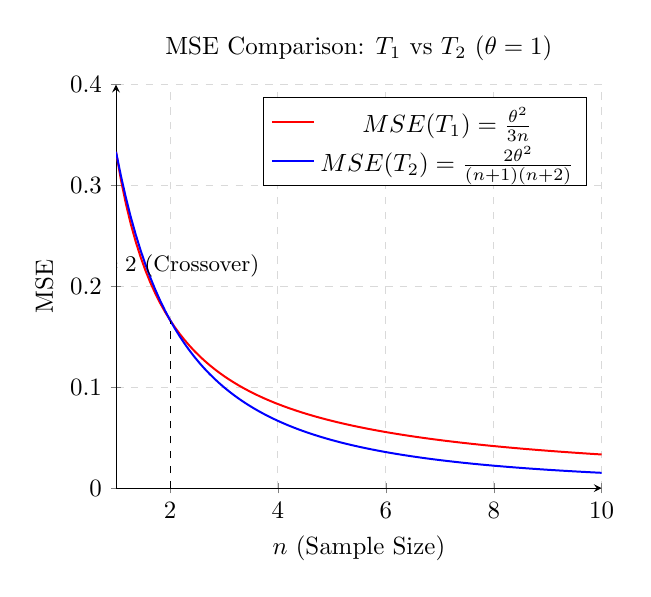
\begin{tikzpicture}[scale=0.9]
\begin{axis}[
    axis lines = left,
    xlabel = {$n$ (Sample Size)},
    ylabel = {MSE},
    domain = 1:10,
    samples = 100,
    ymin = 0, ymax = 0.4,
    legend pos = north east,
    grid = major,
    grid style = {dashed, gray!30},
    title = {MSE Comparison: $T_1$ vs $T_2$ ($\theta=1$)}
]
    % MSE(T1) = 1/(3n)
    \addplot [
        thick,
        color=red,
    ] {1/(3*x)};
    \addlegendentry{$MSE(T_1) = \frac{\theta^2}{3n}$}

    % MSE(T2) = 2/((n+1)(n+2))
    \addplot [
        thick,
        color=blue,
    ] {2/((x+1)*(x+2))};
    \addlegendentry{$MSE(T_2) = \frac{2\theta^2}{(n+1)(n+2)}$}
    
    % Highlight the crossover at n=2
    \draw [dashed, black] (axis cs:2,0) -- (axis cs:2,0.166);
    \node [anchor=south] at (axis cs:2,0.2) {\small $n=2$ (Crossover)};

\end{axis}
\end{tikzpicture}
\caption{The $MSE(T_2)$ decays at a rate of $1/n^2$, making it more efficient than $T_1$ for all $n > 2$.}
\end{figure}








\begin{definition}
The relative efficiency of an unbiased estimator $T$ of $\tau(\theta)$ to another unbiased estimator $T^*$ of $\tau(\theta)$ is given by \[\operatorname{re}(T,T^{*}) = \frac{\operatorname{Var}(T^*)}{\operatorname{Var}(T)}.\]
An unbiased estimator $T^*$ of $\tau(\theta)$ is said to be efficient if re$(T,T^*) \leq 1$ for all unbiased estimators $T$ of $\tau(\theta)$ and all $\theta \in \Omega$.

The efficiency of an unbiased estimator $T$ of $\tau(\theta)$ is given by \[e(T) = \operatorname{re}(T,T^*) = \frac{\operatorname{Var}(T^*)}{\operatorname{Var}(T)}\] if $T^*$ is an efficient estimator of $\tau(\theta)$.
\end{definition}



\begin{definition}
Let $X_1, X_2, \cdots, X_n$ be a random sample of size $n$ from $f(x;\theta)$. An estimator $T^*$ of $\tau(\theta)$ is called a uniformly minimum variance unbiased estimator (UMVUE) of $\tau(\theta)$ if:
\begin{enumerate}
\item[(i).] $T^*$ is unbiased for $\tau(\theta)$, and
\item[(ii).] $\operatorname{Var}(T^*) \leq \operatorname{Var}(T)$, for any other unbiased estimator $T$ of $\tau(\theta)$, for all $\theta \in \Omega$.
\end{enumerate}
\end{definition}



\begin{thm}[\textbf{Cramer-Rao Inequality}]
Let $X_1, X_2, \cdots, X_n$ be a random sample from $f(x;\theta), \, \theta \in \Omega$. Let $T$ be any unbiased estimator for $\tau(\theta)$. Then, under regularity conditions, \[\operatorname{Var}(T)\geq \frac{\left[\tau'(\theta)\right]^2}{J(\theta)}\] where $J(\theta)$ is the Fisher information function.
\end{thm}



\begin{note}
\textbf{ }
\begin{enumerate}
\item The number $\frac{\left[\tau'(\theta)\right]^2}{J(\theta)}$ is called the Cramer-Rao lower bound (CRLB).
\item If an estimator can be found that attains the CRLB then that estimator is a UMVUE for $\tau(\theta)$.
\item If equality holds then $T$ is called an efficient estimator of $\tau(\theta)$.
\item The ratio of the CRLB to the variance of an unbiased estimator is called the efficiency of the estimator. i.e \[e(T) = \frac{\operatorname{CRLB}}{\operatorname{Var}(T)}.\]
\end{enumerate}
\end{note}



\begin{example}
Let $X_1, X_2, \cdots, X_n$ be a random sample from \[f(x;\theta) = \frac{1}{\theta}e^{-\frac{x}{\theta}}\, , \quad x > 0.\] Let $T_1 = \overline{X}$ and $T_2 = nX_{(1)}$ be estimator of $\theta$.
\begin{enumerate}
\item[(a).] Show that $T_1$ and $T_2$ are unbiased estimators of $\theta$.
\begin{proof}[\textbf{\textit{Solution}}]
\begin{align*}
E(T_1)  = E(\overline{X})
& = E(X)\\
%& = \int^{\infty}_0x\, \frac{1}{\theta}e^{-\frac{x}{\theta}}\, dx\\
& = \int^{\infty}_0 \frac{x}{\theta}e^{-\frac{x}{\theta}}\, dx\\
& = \theta\int^{\infty}_0 m e^{-m}\, dm\, , \quad\quad\quad \text{letting}\quad m = \frac{x}{\theta}\\
& =\theta.
\end{align*}
Therefore, $T_1$ is an unbiased estimator of $\theta$.
\[E(T_2) = E[nX_{(1)}] = nE[X_{(1)}]\]
\[f_{X_{(1)}}(y) = n(1-F_X(y))^{n-1}\, f_X(y)\]
\[F_X(x)  = \int_0^x f(t) \, dt = \int^x_0 \frac{1}{\theta}e^{-\frac{t}{\theta}}\, dt = -e^{-\frac{t}{\theta}}\Big|^x_0  = 1 - e^{-\frac{x}{\theta}}.\]
\[f_{X_{(1)}}(y) = n\left[1 - 1 + e^{-\frac{y}{\theta}}\right]^{n-1}\, \frac{1}{\theta}e^{-\frac{y}{\theta}} = \frac{n}{\theta}e^{-\frac{ny}{\theta}}\, , \quad y >0\]
Then
\begin{align*}
E[X_{(1)}] & = \int^{\infty}_0y\, \frac{n}{\theta}e^{-\frac{ny}{\theta}}\, dy\\
& = \int^{\infty}_0 \frac{ny}{\theta}e^{-\frac{ny}{\theta}}\, dy\\
& = \frac{\theta}{n}\, \int^{\infty}_0me^{-m}\,  dm\, , \quad\quad\quad\text{letting}\quad m = \frac{ny}{\theta}\\
& = \frac{\theta}{n}.
\end{align*}
Therefore \[E(T_2) = n\, \frac{\theta}{n} = \theta.\]
\end{proof}



\item[(b).] Find the CRLB for the variances of unbiased estimators of $\theta$.
\begin{proof}[\textbf{\textit{Solution}}]
CRLB $= \frac{\left[\tau'(\theta)\right]^2}{J(\theta)}$, \quad $\tau(\theta) = \theta$ implies that $\tau'(\theta) = 1.$
\[f(x;\theta) = \frac{1}{\theta}e^{-\frac{x}{\theta}}\]
\[\ln f(x;\theta) = -\frac{x}{\theta}-\ln \theta\]
\[\frac{\partial}{\partial\theta}\ln f(x;\theta) = \frac{x}{\theta^2}- \frac{1}{\theta}\]
\[\frac{\partial^2}{\partial\theta^2}\ln f(x;\theta) = -\frac{2x}{\theta^3}+ \frac{1}{\theta^2}\]
So that
\begin{align*}
J(\theta) & = nE\left[-\frac{\partial^2}{\partial \theta^2}\ln f(x;\theta)\right]\\
& = n\, E\left[\frac{2X}{\theta^2}-\frac{1}{\theta^2}\right]\\
& = n\, \left[\frac{2\, E(X)}{\theta^3}-\frac{1}{\theta^2}\right]\\
& = n\, \left[\frac{2\theta}{\theta^3}- \frac{1}{\theta^2}\right]\\
& = \frac{n}{\theta^2}.
\end{align*}
Therefore, \[\operatorname{CRLB} = \frac{1}{J(\theta)} = \frac{1}{n/\theta^2} = \frac{\theta^2}{n}.\]
\end{proof}





\item[(c).] Is $T_1$ a U.M.V.U.E of $\theta$?
\begin{proof}[\textbf{\textit{Solution}}]
$\operatorname{Var}(T_1) = \operatorname{Var}(\overline{X}) = \frac{1}{n}\operatorname{Var}(X).$
\[\operatorname{Var}(X) = E(X^2) - [E(X)]^2\]
\begin{align*}
E(X^2) & = \int_0^{\infty} x^2 \, \frac{1}{\theta}e^{-\frac{x}{\theta}}\, dx\\
& =\frac{1}{\theta}\int^{\infty}_0(\theta m)^2 e^{-m} \, \theta \, dm\, ,\quad\quad\quad \text{letting} \quad m = \frac{x}{\theta}\\
& = \frac{1}{\theta}\, \theta^2\, \theta\underbrace{\int^{\infty}_0 m^2 e^{-m}\, dm}_{2!}\\
& = 2\theta^2.
\end{align*}
Hence \[\operatorname{Var}(X) = 2\theta^2 - \theta^2 = \theta^2.\]
Therefore \[\operatorname{Var}(T_1) = \frac{\theta^2}{n}.\]
i.e. $T_1$ attains the CRLB

Therefore, $T_1 = \overline{X}$ is the U.M.V.U.E for $\theta$.
\end{proof}





\item[  ] Is $T_2$ a U.M.V.U.E of $\theta$?
\begin{proof}[\textbf{\textit{Solution}}]
$\operatorname{Var}(T_2) = \operatorname{Var}(nX_{(1)}) = n^2\, \operatorname{Var}(X_{(1)})$
\begin{align*}
E\left[X_{(1)}\right]^2 & = \int^{\infty}_0 y^2\, \frac{n}{\theta}\, e^{-\frac{ny}{\theta}}\, dy\\
& = \frac{\theta}{n}\int^{\infty}_0 \left(\frac{ny}{\theta}\right)^2\, e^{-\frac{ny}{\theta}}\, dy\\
& = \frac{\theta}{n}\,\frac{\theta}{n} \underbrace{\int^{\infty}_0m^2e^{-m}\, dm}_{2!}\, ,\quad\quad\quad \text{letting}\quad m = \frac{ny}{\theta}\\
& = \frac{2\theta^2}{n^2}.
\end{align*}
Hence \[\operatorname{Var}(X_{(1)} = \frac{2\theta^2}{n^2}- \frac{\theta^2}{n^2} = \frac{\theta^2}{n^2}.\]
Therefore \[\operatorname{Var}(T_2) = \frac{n^2 \theta^2}{n^2} = \theta^2.\]
i.e $T_2$ does not attain the CRLB. Therefore, $T_2 = n\, X_{(1)}$ is not a U.M.V.U.E for $\theta$.
\end{proof}




\item[(d).] Find the efficiency of $T_1$.
\begin{proof}[\textit{Solution.}]
\[e(T_1) = \frac{\operatorname{CRLB}}{\operatorname{Var}(T_1)} = \frac{\theta^2/n}{\theta^2/n} = 1.\]
That is, $T_1$ is an efficient estimator of $\theta$.
\end{proof}


\item[    ] Find the efficiency of $T_2$.
\begin{proof}[\textit{Solution.}]
\[e(T_2) = \frac{\operatorname{CRLB}}{\operatorname{Var}(T_2)} = \frac{\theta^2/n}{\theta^2} = \frac{1}{n}.\]
\end{proof}


\item[(e).] Find the CRLB for the variances of unbiased estimators of $\frac{1}{\theta}$.
\begin{proof}[\textit{Solution.}]
$\operatorname{CRLB} = \frac{\left[\tau'(\theta)\right]^2}{J(\theta)}$
\[\tau(\theta) = \frac{1}{\theta}\]
\[\tau'(\theta) = -\frac{1}{\theta^2}\]
\[\operatorname{CRLB} = \frac{(-1/\theta^2)^2}{n/\theta^2} = \frac{1}{\theta^2}\, \cdot\, \frac{\theta^2}{n} = \frac{1}{n\theta^2}\]
\end{proof}
\end{enumerate}
\end{example}



\begin{definition}
A sequence $\{T_n\}$ of estimators of $\tau(\theta)$ is said to be asymptotically unbiased if \[\lim_{n\rightarrow \infty} E(T_n) = \tau(\theta) \quad \text{for all}\quad \theta \in \Omega.\] (i.e $\lim_{n\rightarrow \infty}\operatorname{bias}(T) = 0)$
\end{definition}



\begin{thm}
A random variable $X_n$ converges in probability to $c$, written $X_n\overset{P}{\longrightarrow}c$, if and only if for every $\varepsilon > 0$, \[\lim_{n\rightarrow \infty}P\left(|X_n - c|<\varepsilon\right) = 1\quad \text{or}\quad \lim_{n\rightarrow \infty}P\left(|X_n - c|> \varepsilon\right)  = 0.\]
\end{thm}




\begin{thm}[\textbf{weak law of large numbers}]
Let $X_1, X_2, \cdots, X_n$ be i.i.d random variables with mean $E(X_i) = \mu$ and finite variance $\operatorname{Var}(X_i) = \sigma^2$. Then $\, \overline{X}_n\overset{P}{\longrightarrow} \mu$.
\end{thm}



\begin{thm}[\textbf{Limit Theorems}]\textbf{ }
\begin{enumerate}
\item If $X_n\overset{P}{\longrightarrow} a$ and $g$ is continuous at $x = a$, then $g(X_n) \overset{P}{\longrightarrow} g(a).$
\item If $X_n\overset{P}{\longrightarrow} a, \quad Y_n\overset{P}{\longrightarrow} b $ and $g(x,y)$ is continuous at $(a,b)$ then $g(X_nY_n)\overset{P}{\longrightarrow} g(a,b)$.
\end{enumerate}
\end{thm}


\begin{thm}
Let $\{T_n\}$ be a sequence of estimators of $\tau(\theta)$. These estimators are said to be consistent estimators of $\tau(\theta)$ if for every $\varepsilon > 0$, \[\lim_{n\rightarrow \infty}P\left(|T_n - \tau(\theta)| < \varepsilon\right) = 1\] for every $\theta \in \Omega$. [i.e. $T_n \overset{P}{\longrightarrow}\tau(\theta)$]
\end{thm}



\begin{thm}
A sequence $\{T_n\}$ of estimators of $\tau(\theta)$ is consistent if and only if it is asymptotically unbiased and \[\lim_{n\rightarrow \infty}\operatorname{Var}(T_n) = 0.\]
\end{thm}



\begin{example}
Let $X_1, X_2, \cdots, X_n$ be a random sample from a $N(\mu,\sigma^2)$ distribution. Let $T = \frac{1}{n}\sum^n_{i=1}(X_i-\overline{X})^2$ be an estimator for $\sigma^2$. Show that 
\begin{enumerate}
\item[(a).] $T$ is an asymptotically  unbiased estimator for $\sigma^2$. 
\begin{proof}[\textit{Solution.}]
\begin{align*}
E(T) & = E\left([\frac{1}{n}\sum^n_{i = 1}(X_i - \overline{X})^2\right]\\
& = E\left[\frac{n - 1}{n}\, \frac{1}{n- 1}\sum^n_{i = 1} (X_i - \overline{X})^2\right]\\
& = \frac{n - 1}{n}E(S^2)\\
& = \frac{n-1}{n}\sigma^2.
\end{align*}
\[\operatorname{bias}(T) = E(T) - \sigma^2 = \frac{n-1}{n}\sigma^2 - \sigma^2 = -\frac{1}{n}\sigma^2 \longrightarrow 0.\]
That is 
\[\lim_{n\rightarrow \infty} \operatorname{bias}(T) = \lim_{n\rightarrow \infty}\left(-\frac{1}{n}\sigma^2\right) = 0.\]
i.e 
\[\lim_{n\rightarrow \infty}E(T) = \lim_{n\rightarrow \infty}\left(\frac{n-1}{n}\sigma^2\right) = \sigma^2 \lim_{n \rightarrow \infty}\left(1 - \frac{1}{n}\right) = \sigma^2.\]
Therefore, $T$ is an asymptotically unbiased estimator for $\sigma^2$.
\end{proof}



\item[(b).] $T$ is a consistent estimator for $\sigma^2$.
\begin{proof}[\textit{Solution}]
\[\operatorname{Var}(T) = \operatorname{Var}\left(\frac{n-1}{n}\, S^2\right) = \left(\frac{n - 1}{n}\right)^2\, \operatorname{Var}(S^2).\]
Recall $\, (n-1)\frac{S^2}{\sigma^2} \thicksim \chi^2(n-1)$
\[\implies\,\, \operatorname{Var}\left[(n-1)\frac{S^2}{\sigma^2}\right] = 2(n-1)\]
\[\frac{(n-1)^2}{\sigma^4}\, \operatorname{Var}(S^2) = 2(n-1)\]
\[\operatorname{Var}(S^2) = \frac{2(n-1)\sigma^4}{(n-1)^2} = \frac{2\sigma^4}{n-1}.\]
Therefore
\[\operatorname{Var}(T) = \frac{(n-1)^2}{n^2}\, \frac{2\sigma^4}{n-1}=\frac{2(n-1)\sigma^4}{n^2}\]
\[\lim_{n\rightarrow \infty}\operatorname{Var}(T) = \lim_{n\rightarrow \infty}\frac{2(n-1)\sigma^4}{n^2} = 2\sigma^4\lim_{n\rightarrow \infty}\left(\frac{1}{n}-\frac{1}{n^2}\right) = 0.\]
i.e $T$ is asymptotically unbiased and $\lim_{n\rightarrow \infty}\operatorname{Var}(T) = 0$. 

Therefore, $T$ is a consistent estimator for $\sigma^2$.
\end{proof}
\end{enumerate}
\end{example}



%%%%%%%%%%%%%%%%%%%%%%%%%%%%%%%%%%%%%%%%%%

\section{Practice problems}

Past assignment questions on estimation. Work each one before opening the solution.

\begin{problem}{Assignment 2}
Let $X_1,X_2,\ldots,X_n$ be a random sample from
$$f(x;\theta)=\theta^2xe^{-\theta x},\qquad x>0,\ \theta>0.$$
Find (a) the method of moments estimator for $\theta$, (b) a sufficient statistic
for $\theta$, (c) the maximum likelihood estimator for $\theta$, (d) the information
function for $\theta$.
\end{problem}

\begin{solution}
Recognise the density first: it is $\text{GAM}(\alpha=2,\ \text{rate }\theta)$, which
saves deriving moments from scratch.

\textbf{(a) Method of moments.} The first population moment is
$$E(X)=\int_0^\infty x\cdot\theta^2xe^{-\theta x}\,dx
=\theta^2\int_0^\infty x^2e^{-\theta x}\,dx=\theta^2\cdot\frac{2}{\theta^3}
=\frac{2}{\theta}.$$
Equating it to the first sample moment $\bar X$,
$$\frac{2}{\theta}=\bar X\quad\implies\quad \tilde\theta=\frac{2}{\bar X}
=\frac{2n}{\sum_{i=1}^n X_i}.$$

\textbf{(b) Sufficient statistic.} The likelihood is
$$L(\theta)=\prod_{i=1}^n\theta^2x_ie^{-\theta x_i}
=\theta^{2n}e^{-\theta\sum x_i}\cdot\prod_{i=1}^n x_i.$$
This is already in the factorisation form $g\!\left(\sum x_i;\theta\right)h(\mathbf{x})$,
with
$$g\!\left(\textstyle\sum x_i;\theta\right)=\theta^{2n}e^{-\theta\sum x_i},
\qquad h(\mathbf{x})=\prod x_i,$$
and $h$ free of $\theta$. By the factorisation criterion
$$T=\sum_{i=1}^n X_i\ \text{ is sufficient for }\theta.$$

\textbf{(c) Maximum likelihood.} Take logarithms:
$$\ell(\theta)=2n\ln\theta+\sum\ln x_i-\theta\sum x_i.$$
$$\frac{d\ell}{d\theta}=\frac{2n}{\theta}-\sum x_i=0
\quad\implies\quad \hat\theta=\frac{2n}{\sum x_i}=\frac{2}{\bar X}.$$
It is a maximum because
$$\frac{d^2\ell}{d\theta^2}=-\frac{2n}{\theta^2}<0\quad\text{for every }\theta>0.$$

\textbf{(d) Information function.} For a single observation,
$$\ln f=2\ln\theta+\ln x-\theta x,\qquad
\frac{\partial\ln f}{\partial\theta}=\frac{2}{\theta}-x,\qquad
\frac{\partial^2\ln f}{\partial\theta^2}=-\frac{2}{\theta^2}.$$
The second derivative is already free of $x$, so taking the expectation changes
nothing:
$$I_1(\theta)=-E\!\left[\frac{\partial^2\ln f}{\partial\theta^2}\right]
=\frac{2}{\theta^2},\qquad\text{and for the sample}\qquad
I_n(\theta)=\frac{2n}{\theta^2}.$$

\begin{note}
The moment estimator and the maximum likelihood estimator coincide here. That is
not a general rule --- it happens because $E(X)$ is a one-to-one function of
$\theta$ and the likelihood equation reduces to the same relation. When they
disagree, it is the maximum likelihood estimator that inherits the good
large-sample properties.
\end{note}

\begin{note}
Part (d) is unusually quick because $\frac{\partial^2\ln f}{\partial\theta^2}$
contains no $x$. In general it does, and the expectation has to be evaluated ---
as it does in the next question.
\end{note}
\end{solution}

\begin{problem}{Assignment 2}
Let $X_1,X_2,\ldots,X_n$ be a random sample from
$$f(x;\theta)=\binom{x-1}{2}\theta^3(1-\theta)^{x-3},\qquad x=3,4,5,\ldots$$
Find (a) the MME for $\theta$, (b) a sufficient statistic for $\theta$, (c) the MLE
for $\theta$, (d) the Fisher information function.
\end{problem}

\begin{solution}
This is the negative binomial in its ``trials until the third success'' form: $X$
counts the trials needed to obtain $3$ successes, each of probability $\theta$. Its
mean is therefore
$$E(X)=\frac{3}{\theta}.$$

\textbf{(a) Method of moments.}
$$\frac{3}{\theta}=\bar X\quad\implies\quad \tilde\theta=\frac{3}{\bar X}
=\frac{3n}{\sum X_i}.$$

\textbf{(b) Sufficient statistic.} The likelihood is
$$L(\theta)=\prod_{i=1}^n\binom{x_i-1}{2}\theta^3(1-\theta)^{x_i-3}
=\underbrace{\theta^{3n}(1-\theta)^{\sum x_i-3n}}_{g\left(\sum x_i;\theta\right)}
\cdot\underbrace{\prod_{i=1}^n\binom{x_i-1}{2}}_{h(\mathbf{x})}.$$
By the factorisation criterion,
$$T=\sum_{i=1}^n X_i\ \text{ is sufficient for }\theta.$$

\textbf{(c) Maximum likelihood.}
$$\ell(\theta)=\sum\ln\binom{x_i-1}{2}+3n\ln\theta+\left(\sum x_i-3n\right)\ln(1-\theta),$$
$$\frac{d\ell}{d\theta}=\frac{3n}{\theta}-\frac{\sum x_i-3n}{1-\theta}=0.$$
Multiplying through by $\theta(1-\theta)$,
$$3n(1-\theta)=\theta\left(\sum x_i-3n\right)
\ \implies\ 3n-3n\theta=\theta\sum x_i-3n\theta
\ \implies\ 3n=\theta\sum x_i,$$
the $3n\theta$ terms cancelling on both sides, so
$$\hat\theta=\frac{3n}{\sum x_i}=\frac{3}{\bar X}.$$

\textbf{(d) Fisher information.} For one observation the terms in $\theta$ are
$$\ln f=\text{constant}+3\ln\theta+(x-3)\ln(1-\theta),$$
$$\frac{\partial\ln f}{\partial\theta}=\frac{3}{\theta}-\frac{x-3}{1-\theta},
\qquad
\frac{\partial^2\ln f}{\partial\theta^2}=-\frac{3}{\theta^2}-\frac{x-3}{(1-\theta)^2}.$$
Now the second derivative \emph{does} involve $x$, so the expectation must be taken.
Since $E(X)=\frac{3}{\theta}$,
$$E(X-3)=\frac{3}{\theta}-3=\frac{3(1-\theta)}{\theta},$$
and therefore
$$I_1(\theta)=-E\!\left[\frac{\partial^2\ln f}{\partial\theta^2}\right]
=\frac{3}{\theta^2}+\frac{1}{(1-\theta)^2}\cdot\frac{3(1-\theta)}{\theta}
=\frac{3}{\theta^2}+\frac{3}{\theta(1-\theta)}.$$
Over the common denominator $\theta^2(1-\theta)$,
$$I_1(\theta)=\frac{3(1-\theta)+3\theta}{\theta^2(1-\theta)}
=\frac{3}{\theta^2(1-\theta)},\qquad
I_n(\theta)=\frac{3n}{\theta^2(1-\theta)}.$$

\begin{note}
The $3n\theta$ terms cancelling in (c) is what makes the likelihood equation
solvable in closed form. Notice also that the answer is $\frac{3}{\bar X}$, again
matching the moment estimator, and that both are just ``three successes divided by
the average number of trials'' --- which is what one would have guessed.
\end{note}
\end{solution}


\begin{problem}{Assignment 2}
Let $Y_1,\ldots,Y_n$ be a random sample from
$$f(y;\mu,\sigma^2)=\frac{1}{y\sqrt{2\pi\sigma^2}}
e^{-\frac{1}{2\sigma^2}(\log y-\mu)^2},\qquad y>0.$$
With $\theta=(\mu,\sigma^2)$, find (a) the sufficient statistic for $\theta$, (b) the
MLE for $\theta$, (c) the information matrix for $\theta$, (d) the MLE for $E(Y)$.
\end{problem}

\begin{solution}
This is the lognormal density. The one observation worth making before any algebra
is that $W=\log Y\sim N(\mu,\sigma^2)$: everything then follows from the normal case.

\textbf{(a) Sufficient statistic.} Writing $w_i=\log y_i$,
$$L(\theta)=\left(2\pi\sigma^2\right)^{-n/2}\left(\prod y_i\right)^{-1}
\exp\!\left(-\frac{1}{2\sigma^2}\sum(w_i-\mu)^2\right).$$
Expanding the square, $\sum(w_i-\mu)^2=\sum w_i^2-2\mu\sum w_i+n\mu^2$, so
$$L(\theta)=\underbrace{\left(2\pi\sigma^2\right)^{-n/2}
\exp\!\left(-\frac{\sum w_i^2-2\mu\sum w_i+n\mu^2}{2\sigma^2}\right)}
_{g\left(\sum w_i,\ \sum w_i^2;\ \theta\right)}
\cdot\underbrace{\left(\prod y_i\right)^{-1}}_{h(\mathbf{y})}.$$
$$\therefore\quad T=\left(\sum_{i=1}^n\log Y_i,\ \sum_{i=1}^n(\log Y_i)^2\right)
\text{ is jointly sufficient for }\theta.$$

\textbf{(b) Maximum likelihood.} These are the normal estimators applied to the
$w_i$:
$$\hat\mu=\frac{1}{n}\sum_{i=1}^n\log Y_i,\qquad
\hat\sigma^2=\frac{1}{n}\sum_{i=1}^n\left(\log Y_i-\hat\mu\right)^2.$$

\textbf{(c) Information matrix.} Again as for the normal in $w$,
$$I(\theta)=n\begin{pmatrix}\frac{1}{\sigma^2} & 0\\[3pt]
0 & \frac{1}{2\sigma^4}\end{pmatrix}.$$
The off-diagonal entries are zero, so $\hat\mu$ and $\hat\sigma^2$ are
asymptotically independent.

\textbf{(d) MLE of $E(Y)$.} For the lognormal,
$$E(Y)=e^{\mu+\frac{\sigma^2}{2}}.$$
By the invariance property of maximum likelihood --- the MLE of $\tau(\theta)$ is
$\tau$ evaluated at the MLE ---
$$\widehat{E(Y)}=e^{\hat\mu+\frac{\hat\sigma^2}{2}}.$$

\begin{note}
Note what $E(Y)$ is \emph{not}: it is not $e^{\hat\mu}$. The $\frac{\sigma^2}{2}$
term is the whole difference between the median of a lognormal, $e^{\mu}$, and its
mean. Reporting $e^{\hat\mu}$ as the estimated mean understates it, and by more the
larger the variance.
\end{note}
\end{solution}

\begin{problem}{Assignment 2}
Let $X_1,\ldots,X_n$ be a random sample from $X\sim\text{UNIF}(0,\theta)$. Let
$T_1=X_{(n)}$ and let $T_2$ be the MME for $\theta$.
\begin{enumerate}
\item[(a).] Find $T_2$. Is it an unbiased estimator of $\theta$?
\item[(b).] Is $T_1$ asymptotically unbiased for $\theta$?
\item[(c).] Show that $T_1$ is a consistent estimator of $\theta$.
\item[(d).] Find the MSE of $T_1$. \quad (e) Find the MSE of $T_2$.
\quad (f) Find $e(T_1,T_2)$.
\end{enumerate}
\end{problem}

\begin{solution}
\textbf{(a).} $E(X)=\frac{\theta}{2}$, so equating to $\bar X$ gives
$$T_2=2\bar X,\qquad E(T_2)=2\cdot\frac{\theta}{2}=\theta.$$
So $T_2$ is \textbf{unbiased}.

\textbf{(b).} The largest order statistic has density
$$g(x)=\frac{nx^{n-1}}{\theta^n},\qquad 0<x<\theta,$$
so
$$E(T_1)=\int_0^\theta x\cdot\frac{nx^{n-1}}{\theta^n}\,dx=\frac{n\theta}{n+1}
\ \longrightarrow\ \theta\quad\text{as }n\to\infty.$$
It is biased for every finite $n$ --- always \emph{under}-estimating, as it must,
since the largest observation cannot exceed $\theta$ --- but
\textbf{asymptotically unbiased}.

\textbf{(c).} Also
$$E\left(T_1^2\right)=\int_0^\theta x^2\cdot\frac{nx^{n-1}}{\theta^n}\,dx
=\frac{n\theta^2}{n+2},$$
so, using the result of (d) below,
$$\text{MSE}(T_1)=\frac{2\theta^2}{(n+1)(n+2)}\ \longrightarrow\ 0
\quad\text{as }n\to\infty.$$
An estimator whose mean squared error tends to zero converges in probability to
$\theta$, so $T_1$ is \textbf{consistent}.

\textbf{(d).} Since $T_1$ is biased, use $\text{MSE}=E\left(T_1^2\right)-2\theta
E(T_1)+\theta^2$:
$$\text{MSE}(T_1)=\frac{n\theta^2}{n+2}-\frac{2n\theta^2}{n+1}+\theta^2
=\theta^2\cdot\frac{n(n+1)-2n(n+2)+(n+1)(n+2)}{(n+1)(n+2)}.$$
The numerator is
$$\left(n^2+n\right)-\left(2n^2+4n\right)+\left(n^2+3n+2\right)=2,$$
the $n^2$ and $n$ terms cancelling completely, so
$$\text{MSE}(T_1)=\frac{2\theta^2}{(n+1)(n+2)}.$$

\textbf{(e).} $T_2$ is unbiased, so its MSE is its variance. With
$\text{Var}(X)=\frac{\theta^2}{12}$,
$$\text{MSE}(T_2)=\text{Var}\left(2\bar X\right)=4\cdot\frac{\theta^2}{12n}
=\frac{\theta^2}{3n}.$$

\textbf{(f).}
$$e(T_1,T_2)=\frac{\text{MSE}(T_2)}{\text{MSE}(T_1)}
=\frac{\frac{\theta^2}{3n}}{\frac{2\theta^2}{(n+1)(n+2)}}
=\frac{(n+1)(n+2)}{6n}.$$

\begin{note}
This is the standard cautionary example. $T_2$ is unbiased and $T_1$ is not, yet
$T_1$ is enormously better: its MSE falls like $\frac{1}{n^2}$ while $T_2$'s falls
only like $\frac{1}{n}$, and the efficiency ratio grows without bound. Unbiasedness
on its own is not a reason to prefer an estimator.
\end{note}
\end{solution}

\begin{problem}{Assignment 2}
Let $X_1,\ldots,X_n$ be a random sample from $f(x;\theta)=\frac{2\theta^2}{x^3}$,
$x>\theta$. Let $T_1$ be the MME and $T_2$ the MLE for $\theta$.
\begin{enumerate}
\item[(a).] Find $T_1$. Is it unbiased for $\theta$? \quad (b) Find $T_2$.
\item[(c).] Show that $T_2$ is asymptotically unbiased.
\item[(d).] Show that $T_2$ is a consistent estimator.
\end{enumerate}
\end{problem}

\begin{solution}
\textbf{(a).}
$$E(X)=\int_\theta^\infty x\cdot\frac{2\theta^2}{x^3}\,dx
=2\theta^2\int_\theta^\infty x^{-2}dx=2\theta^2\cdot\frac{1}{\theta}=2\theta.$$
Setting $2\theta=\bar X$,
$$T_1=\frac{\bar X}{2},\qquad E(T_1)=\frac{2\theta}{2}=\theta,$$
so $T_1$ is \textbf{unbiased}.

\textbf{(b).} The likelihood is
$$L(\theta)=\frac{2^n\theta^{2n}}{\prod x_i^3},\qquad\text{valid only while }
\theta<x_i\text{ for every }i.$$
Differentiating is useless here: $L$ is \emph{increasing} in $\theta$, so it is made
as large as the constraint permits. The binding constraint is
$\theta\leq\min_i x_i$, hence
$$T_2=X_{(1)}=\min_i X_i.$$

\textbf{(c).} The smallest order statistic has density
$$g(x)=n\left[1-F(x)\right]^{n-1}f(x)
=n\left(\frac{\theta^2}{x^2}\right)^{n-1}\cdot\frac{2\theta^2}{x^3}
=\frac{2n\theta^{2n}}{x^{2n+1}},\qquad x>\theta,$$
using $F(x)=1-\frac{\theta^2}{x^2}$. Then
$$E(T_2)=\int_\theta^\infty x\cdot\frac{2n\theta^{2n}}{x^{2n+1}}\,dx
=2n\theta^{2n}\int_\theta^\infty x^{-2n}dx
=2n\theta^{2n}\cdot\frac{\theta^{1-2n}}{2n-1}=\frac{2n\theta}{2n-1}.$$
As $n\to\infty$ this tends to $\theta$, so $T_2$ is \textbf{asymptotically
unbiased}. Note it over-estimates, the mirror image of the uniform case, because
the smallest observation must exceed $\theta$.

\textbf{(d).} By the same integral with $x^2$,
$$E\left(T_2^2\right)=2n\theta^{2n}\int_\theta^\infty x^{1-2n}dx
=\frac{2n\theta^2}{2n-2}=\frac{n\theta^2}{n-1}.$$
Hence
$$\text{MSE}(T_2)=\frac{n\theta^2}{n-1}-\frac{4n\theta^2}{2n-1}+\theta^2
=\frac{\theta^2}{(n-1)(2n-1)}\ \longrightarrow\ 0,$$
so $T_2$ is \textbf{consistent}.

\begin{note}
Part (b) is the one to be careful with. Setting $\frac{d\ell}{d\theta}=0$ finds
nothing, because the likelihood has no interior stationary point --- the maximum is
at the boundary of the parameter space. Whenever the range of $x$ depends on
$\theta$, look at the constraint before differentiating.
\end{note}
\end{solution}

\begin{problem}{Assignment 2}
Let $X_1,\ldots,X_n$ be a random sample from $f(x;\theta)=\theta e^{-\theta x}$,
$x>0$.
\begin{enumerate}
\item[(a).] Find the MLE of $\theta$.
\item[(b).] Find the MLE of $\frac{1}{\theta}$. Is it unbiased?
\item[(c).] Is the MLE of $\frac{1}{\theta}$ a U.M.V.U.E.?
\item[(d).] Is the MLE of $\theta$ consistent? \quad (e) Is the MLE of
$\frac{1}{\theta}$ consistent?
\end{enumerate}
\end{problem}

\begin{solution}
\textbf{(a).} $\ell(\theta)=n\ln\theta-\theta\sum x_i$, so
$$\frac{d\ell}{d\theta}=\frac{n}{\theta}-\sum x_i=0\quad\implies\quad
\hat\theta=\frac{n}{\sum X_i}=\frac{1}{\bar X},$$
a maximum since $\frac{d^2\ell}{d\theta^2}=-\frac{n}{\theta^2}<0$.

\textbf{(b).} By invariance, the MLE of $\frac{1}{\theta}$ is
$\frac{1}{\hat\theta}=\bar X$. Since $E(X)=\frac{1}{\theta}$,
$$E\left(\bar X\right)=\frac{1}{\theta},$$
so it is \textbf{unbiased}.

\textbf{(c).} The exponential family here has $T=\sum X_i$ as a complete sufficient
statistic for $\theta$. Now $\bar X=\frac{T}{n}$ is a function of $T$ alone and is
unbiased for $\frac{1}{\theta}$. By the Lehmann--Scheff\'e theorem an unbiased
function of a complete sufficient statistic is the unique UMVUE, so
$$\bar X\ \text{ is the U.M.V.U.E. of }\ \frac{1}{\theta}.$$

\textbf{(d) and (e).} By the weak law of large numbers $\bar X\xrightarrow{P}
E(X)=\frac{1}{\theta}$, so the estimator in (b) is \textbf{consistent}. Since
$g(u)=\frac{1}{u}$ is continuous at $u=\frac{1}{\theta}\neq 0$, the continuous
mapping theorem gives
$$\hat\theta=\frac{1}{\bar X}\xrightarrow{P}\theta,$$
so the estimator in (a) is \textbf{consistent} as well.

\begin{note}
Invariance transfers straight through maximum likelihood but \emph{not} through
unbiasedness. Here $\bar X$ is unbiased for $\frac{1}{\theta}$ while
$\frac{1}{\bar X}$ is \emph{not} unbiased for $\theta$ --- in fact
$E\left(\frac{1}{\bar X}\right)=\frac{n\theta}{n-1}$. Consistency, by contrast,
does transfer, which is what (d) uses.
\end{note}
\end{solution}

\begin{problem}{Assignment 2}
Let $X_1,\ldots,X_n$ be a random sample from
$f(x;\theta)=\frac{e^{-\theta}\theta^x}{x!}$, $x=0,1,2,\ldots$
\begin{enumerate}
\item[(a).] Find the MLE of $\theta$.
\item[(b).] Find the CRLB for the variances of unbiased estimators of $\theta$.
\item[(c).] Is the MLE of $\theta$ a U.M.V.U.E.?
\item[(d).] Find the CRLB for variances of unbiased estimators of $e^{-\theta}$.
\item[(e).] Show that $T=\left(\frac{n-1}{n}\right)^{\sum_{i=1}^nX_i}$ is unbiased
for $e^{-\theta}$. \quad (f) Find the efficiency of $T$.
\end{enumerate}
\end{problem}

\begin{solution}
\textbf{(a).} $\ell(\theta)=-n\theta+\ln\theta\sum x_i-\sum\ln x_i!$, so
$$\frac{d\ell}{d\theta}=-n+\frac{\sum x_i}{\theta}=0\quad\implies\quad
\hat\theta=\bar X.$$

\textbf{(b).} From $\ln f=-\theta+x\ln\theta-\ln x!$,
$$\frac{\partial^2\ln f}{\partial\theta^2}=-\frac{x}{\theta^2},\qquad
I_1(\theta)=-E\!\left[-\frac{X}{\theta^2}\right]=\frac{\theta}{\theta^2}
=\frac{1}{\theta}.$$
$$\therefore\quad \text{CRLB}=\frac{1}{nI_1(\theta)}=\frac{\theta}{n}.$$

\textbf{(c).} $\bar X$ is unbiased for $\theta$ and
$\text{Var}\left(\bar X\right)=\frac{\theta}{n}$, which \emph{equals} the bound. An
unbiased estimator attaining the CRLB has the smallest possible variance, so
$\bar X$ is the \textbf{U.M.V.U.E.} of $\theta$.

\textbf{(d).} For $\tau(\theta)=e^{-\theta}$ we have
$\tau'(\theta)=-e^{-\theta}$, and the bound for a function of $\theta$ is
$$\text{CRLB}=\frac{\left[\tau'(\theta)\right]^2}{nI_1(\theta)}
=\frac{e^{-2\theta}}{\frac{n}{\theta}}=\frac{\theta e^{-2\theta}}{n}.$$

\textbf{(e).} Since $\sum X_i\sim\text{POI}(n\theta)$, its probability generating
function is $E\left(s^{\sum X_i}\right)=e^{n\theta(s-1)}$. Putting
$s=\frac{n-1}{n}$,
$$E(T)=e^{n\theta\left(\frac{n-1}{n}-1\right)}
=e^{n\theta\left(-\frac{1}{n}\right)}=e^{-\theta},$$
so $T$ is \textbf{unbiased} for $e^{-\theta}$.

\textbf{(f).} Using the same generating function with $s^2$,
$$E\left(T^2\right)=e^{n\theta\left(\left(\frac{n-1}{n}\right)^2-1\right)}
=e^{n\theta\cdot\frac{1-2n}{n^2}}=e^{-2\theta+\frac{\theta}{n}},$$
$$\text{Var}(T)=e^{-2\theta+\frac{\theta}{n}}-e^{-2\theta}
=e^{-2\theta}\left(e^{\theta/n}-1\right).$$
Therefore
$$\text{eff}(T)=\frac{\text{CRLB}}{\text{Var}(T)}
=\frac{\frac{\theta e^{-2\theta}}{n}}{e^{-2\theta}\left(e^{\theta/n}-1\right)}
=\frac{\theta}{n\left(e^{\theta/n}-1\right)}.$$

\begin{note}
$T$ does not attain the bound, so it is not efficient for any finite $n$. But for
large $n$ the exponent $\frac{\theta}{n}$ is small and
$e^{\theta/n}-1\approx\frac{\theta}{n}$, which makes the efficiency tend to $1$:
$T$ is \emph{asymptotically} efficient.
\end{note}
\end{solution}

\begin{problem}{Assignment 2}
Let $X_1,\ldots,X_n$ be a random sample from
$$f(x;\theta)=\frac{1}{2^\theta\Gamma(\theta)}x^{\theta-1}e^{-\frac{x}{2}},
\qquad x>0.$$
Let $T_1$ be the MME and $T_2$ the MLE for $\theta$. Find (a) $T_1$, (b) $T_2$,
(c) the MSE of $T_1$.
\end{problem}

\begin{solution}
This is $\text{GAM}(\alpha=\theta,\ \beta=2)$: shape unknown, scale known and equal
to $2$. So $E(X)=2\theta$ and $\text{Var}(X)=4\theta$.

\textbf{(a).} Equating $E(X)=2\theta$ to $\bar X$,
$$T_1=\frac{\bar X}{2}.$$

\textbf{(b).} The log-likelihood is
$$\ell(\theta)=-n\theta\ln 2-n\ln\Gamma(\theta)+(\theta-1)\sum\ln x_i
-\frac{1}{2}\sum x_i,$$
$$\frac{d\ell}{d\theta}=-n\ln 2-n\psi(\theta)+\sum\ln x_i=0,$$
where $\psi=\frac{\Gamma'}{\Gamma}$ is the digamma function. So $T_2$ solves
$$\psi(\theta)=\frac{1}{n}\sum_{i=1}^n\ln x_i-\ln 2.$$
There is no closed form: $\psi$ cannot be inverted in elementary functions, so
$T_2$ must be obtained numerically --- by Newton's method, as in Section 2.4.

\textbf{(c).} $T_1$ is unbiased, since
$E\left(\frac{\bar X}{2}\right)=\frac{2\theta}{2}=\theta$, so its MSE is its
variance:
$$\text{MSE}(T_1)=\text{Var}\!\left(\frac{\bar X}{2}\right)
=\frac{1}{4}\cdot\frac{\text{Var}(X)}{n}=\frac{1}{4}\cdot\frac{4\theta}{n}
=\frac{\theta}{n}.$$

\begin{note}
This is the standard case where the two methods genuinely part company. The moment
estimator is immediate and has a clean MSE; the likelihood estimator has no closed
form at all. That is the usual trade --- moments are easy to write down, maximum
likelihood is usually better behaved, and when the likelihood equation will not
solve, the moment estimator makes a good starting value for the iteration.
\end{note}
\end{solution}


\begin{problem}{Assignment 2.2}
Let $X_1,\ldots,X_n$ be a random sample from
$$f_X(x;\alpha,\lambda)=\lambda\frac{(\lambda x)^{\alpha-1}e^{-\lambda x}}
{\Gamma(\alpha)},\qquad \alpha>0,\ \lambda>0,\ x>0.$$
Find (i) joint sufficient statistics for $\theta=(\alpha,\lambda)$, (ii) the MLE
for $\lambda$ if $\alpha=4$, (iii) the Cram\'er--Rao lower bound for $\lambda$ if
$\alpha=4$, (iv) the UMVUE for $\lambda$ if it exists when $\alpha=4$.
\end{problem}

\begin{solution}
\textbf{(i).} The likelihood is
$$L=\frac{\lambda^{n\alpha}}{\Gamma(\alpha)^n}
\left(\prod x_i\right)^{\alpha-1}e^{-\lambda\sum x_i}.$$
Both $\prod x_i$ and $\sum x_i$ appear, and neither can be dispensed with while
$\alpha$ is unknown, so
$$T=\left(\sum_{i=1}^nX_i,\ \prod_{i=1}^nX_i\right)
\quad\text{--- equivalently }\left(\sum X_i,\ \sum\ln X_i\right)\text{ ---}$$
is jointly sufficient for $(\alpha,\lambda)$.

\textbf{(ii).} With $\alpha=4$ the density is
$f(x)=\frac{\lambda^4x^3e^{-\lambda x}}{6}$, so
$$\ell(\lambda)=4n\ln\lambda+3\sum\ln x_i-\lambda\sum x_i-n\ln 6,$$
$$\frac{d\ell}{d\lambda}=\frac{4n}{\lambda}-\sum x_i=0
\quad\implies\quad \hat\lambda=\frac{4n}{\sum X_i}=\frac{4}{\bar X}.$$

\textbf{(iii).} From $\ln f=4\ln\lambda+3\ln x-\lambda x-\ln 6$,
$$\frac{\partial^2\ln f}{\partial\lambda^2}=-\frac{4}{\lambda^2},\qquad
I_1(\lambda)=\frac{4}{\lambda^2},\qquad
\text{CRLB}=\frac{1}{nI_1(\lambda)}=\frac{\lambda^2}{4n}.$$

\textbf{(iv).} With $\alpha$ known, this is a one-parameter exponential family and
$T=\sum X_i$ is a \emph{complete} sufficient statistic. Since each
$X_i\sim\text{GAM}(4,\lambda)$, we have $T\sim\text{GAM}(4n,\lambda)$, and
$$E\!\left(\frac{1}{T}\right)
=\int_0^\infty\frac{1}{t}\cdot\frac{\lambda^{4n}t^{4n-1}e^{-\lambda t}}
{\Gamma(4n)}\,dt=\frac{\lambda\,\Gamma(4n-1)}{\Gamma(4n)}=\frac{\lambda}{4n-1}.$$
So the MLE $\frac{4n}{T}$ is \emph{biased}, with
$E\!\left(\frac{4n}{T}\right)=\frac{4n\lambda}{4n-1}$. Correcting the constant,
$$E\!\left(\frac{4n-1}{T}\right)=\lambda,$$
and $\frac{4n-1}{T}$ is a function of the complete sufficient statistic alone. By
the Lehmann--Scheff\'e theorem,
$$\text{UMVUE of }\lambda\ =\ \frac{4n-1}{\sum_{i=1}^nX_i}.$$

\begin{note}
The UMVUE does \emph{not} attain the Cram\'er--Rao bound here. Using
$E\!\left(\frac{1}{T^2}\right)=\frac{\lambda^2}{(4n-1)(4n-2)}$,
$$\text{Var}\!\left(\frac{4n-1}{T}\right)=\frac{\lambda^2}{4n-2}
\quad>\quad \frac{\lambda^2}{4n}=\text{CRLB},$$
the gap being $\frac{\lambda^2}{4n(2n-1)}$. So ``minimum variance among unbiased
estimators'' and ``attains the CRLB'' are not the same statement --- the bound is
simply not always achievable, and an estimator can be the best there is without
reaching it.
\end{note}
\end{solution}

\begin{problem}{Assignment 2.2}
Let $X_1,\ldots,X_n$ be a random sample from
$f_X(x;\lambda)=\frac{\lambda^xe^{-\lambda}}{x!}$, $x=0,1,2,\ldots$
Find (i) a sufficient statistic for $\lambda$, (ii) the efficiency of the MLE for
$\lambda$, (iii) the relative efficiency of the MLE to $W=X_1$.
\end{problem}

\begin{solution}
\textbf{(i).} The likelihood is
$$L=\frac{\lambda^{\sum x_i}e^{-n\lambda}}{\prod x_i!}
=\underbrace{\lambda^{\sum x_i}e^{-n\lambda}}_{g\left(\sum x_i;\lambda\right)}
\cdot\underbrace{\frac{1}{\prod x_i!}}_{h(\mathbf{x})},$$
so $T=\sum_{i=1}^nX_i$ is sufficient for $\lambda$.

\textbf{(ii).} The MLE is $\hat\lambda=\bar X$, with
$\text{Var}\left(\bar X\right)=\frac{\lambda}{n}$. From
$\frac{\partial^2\ln f}{\partial\lambda^2}=-\frac{x}{\lambda^2}$ we get
$I_1(\lambda)=\frac{1}{\lambda}$ and $\text{CRLB}=\frac{\lambda}{n}$. Hence
$$\text{eff}\left(\hat\lambda\right)
=\frac{\text{CRLB}}{\text{Var}\left(\bar X\right)}
=\frac{\lambda/n}{\lambda/n}=1.$$
The MLE is \textbf{efficient} --- it attains the bound exactly.

\textbf{(iii).} $W=X_1$ is also unbiased for $\lambda$, since $E(X_1)=\lambda$, but
it throws away $n-1$ of the observations. With $\text{Var}(W)=\lambda$,
$$\text{RE}\left(\hat\lambda,W\right)
=\frac{\text{Var}(W)}{\text{Var}\left(\hat\lambda\right)}
=\frac{\lambda}{\lambda/n}=n.$$
The sample mean is $n$ times as efficient as a single observation.

\begin{note}
Contrast this with the previous question. There the UMVUE fell short of the bound;
here the MLE meets it exactly. The Poisson mean is one of the cases where the
score function factors as $I(\lambda)\left(\bar x-\lambda\right)$, and that
proportionality is precisely the condition for equality in the Cram\'er--Rao
inequality.
\end{note}
\end{solution}

\begin{problem}{Assignment 2.2}
Let $X_1,\ldots,X_n$ be a random sample from
$$f_X(x;\theta)=\frac{\theta}{(1+x)^{\theta+1}},\qquad x>0,\ \theta>0.$$
Find (i) a sufficient statistic for $\theta$, (ii) the Cram\'er--Rao lower bound
for $\theta$.
\end{problem}

\begin{solution}
\textbf{(i).} Write the likelihood with the product in the exponent:
$$L=\frac{\theta^n}{\prod(1+x_i)^{\theta+1}}
=\theta^n\exp\!\left(-(\theta+1)\sum\ln(1+x_i)\right).$$
This depends on the sample only through $\sum\ln(1+x_i)$, so
$$T=\sum_{i=1}^n\ln\left(1+X_i\right)\ \text{ is sufficient for }\theta.$$

\textbf{(ii).} From $\ln f=\ln\theta-(\theta+1)\ln(1+x)$,
$$\frac{\partial\ln f}{\partial\theta}=\frac{1}{\theta}-\ln(1+x),\qquad
\frac{\partial^2\ln f}{\partial\theta^2}=-\frac{1}{\theta^2}.$$
The second derivative is free of $x$, so
$$I_1(\theta)=\frac{1}{\theta^2},\qquad
\text{CRLB}=\frac{1}{nI_1(\theta)}=\frac{\theta^2}{n}.$$

\begin{note}
The substitution $Y=\ln(1+X)$ makes this transparent. Since
$P(X>x)=(1+x)^{-\theta}$,
$$P(Y>y)=P\!\left(X>e^y-1\right)=e^{-\theta y},$$
so $Y\sim\text{EXP}(\theta)$ with $E(Y)=\frac{1}{\theta}$. That is why the
sufficient statistic is a sum of logarithms, and it confirms the score has mean
zero: $E\!\left[\frac{1}{\theta}-\ln(1+X)\right]=\frac{1}{\theta}-\frac{1}{\theta}=0$,
as it must.
\end{note}
\end{solution}

\chapter{Hypothesis Testing}

\section{Introduction}
\vspace{-15pt}
In scientific research, we often need to evaluate the validity of theories regarding physical phenomena. Hypothesis testing is the formal process of deciding whether a claim about a population is supported by sample evidence. Because experimental measurements are subject to random error, any decision we make is also subject to error. The goal of statistical testing is to ensure these errors occur at a controlled, preset rate.


\begin{definition}
A statistical hypothesis is a statement concerning the distribution of a random variable $X$, typically specified by a parameter $\theta$. We denote the hypothesis as $H: \theta \in \Omega_0$, where $\Omega_0$ is a subset of the parameter space $\Omega$.
\begin{itemize}
\item \textit{Simple Hypothesis:} A hypothesis that specifies the distribution completely (contains only one member).
\item \textit{Composite Hypothesis:} A hypothesis that does not specify the distribution completely.
\end{itemize}
\end{definition}



\begin{example}
If $X \sim N(\mu, \sigma^2)$:
\begin{itemize}
\item $H: \mu = 4, \sigma^2 = 16$ is a simple hypothesis.
\item $H: \mu = 4, \sigma^2 > 0$ is a composite hypothesis (because $\sigma^2$ is not fixed).
\end{itemize}
\end{example}


\begin{definition}
A test is a rule that tells us whether to reject the null hypothesis ($H_0$) based on observed data. This usually involves a test statistic $T = t(X_1, \dots, X_n)$ and a critical region $R$.
\end{definition}





\begin{note}
The four-step procedure:
\begin{enumerate}
\item State the Hypotheses: 
   \begin{itemize}
   \item  $H_0: \theta \in \Omega_0$ (Null Hypothesis)
   \item $H_1: \theta \in \Omega_1$ (Alternative Hypothesis)
   \end{itemize}
\item Choose a Decision Rule: Define the rejection region $R$, such as $$R = \{ (x_1, \dots, x_n) : t(x) \geq c \}.$$
\item Collect Data: Obtain the sample measurements.
\item Make a Decision: If the observed $t(x)$ falls in $R$, reject $H_0$; otherwise, do not reject $H_0$.
\end{enumerate}
\end{note}










\begin{definition}
The critical region for a test of hypothesis is the subset of the sample space that corresponds to rejecting the null hypothesis.
\end{definition}


\begin{definition}
The power function of a test with critical region $R$ is the function $$\pi(\theta) = P_{\theta}(X\in R)$$ or the probability of rejecting $H_0$ when the true value of the parameter is $\theta$.
\end{definition}



\begin{remark}
When performing a test of $H_0$ versus $H_1$ one may arrive at the correct decision or may commit one of the two kinds of errors.
\begin{table}[H]
\centering
\caption{The Decision Matrix (The State of Mother Nature vs. Statistical Decision)}
\renewcommand{\arraystretch}{1.8} % Increases row height for clarity
\begin{tabular}{|c|m{4cm}|m{4cm}|}
\hline
\multirow{2}{*}{\textbf{Decision}} & \multicolumn{2}{c|}{\textbf{Mother Nature (Truth)}} \\ \cline{2-3} 
 & \centering \textbf{$H_0$ is True} & \centering \textbf{$H_0$ is False ($H_a$ is True)} \tabularnewline \hline
\textbf{Accept $H_0$} & \centering \checkmark \\ Correct Decision \\ Prob $= 1 - \alpha$ & \centering \textbf{Type II Error ($\beta$)} \\ Failing to detect an effect \tabularnewline \hline
\textbf{Reject $H_0$} & \centering \textbf{Type I Error ($\alpha$)} \\ False Positive \\ (Significance Level) & \centering \checkmark \\ Correct Decision \\ \textbf{Power} ($1 - \beta$) \tabularnewline \hline
\end{tabular}
\end{table}





\begin{enumerate}
\item[(a).] Type I error: rejecting $H_0$ when $H_0$ is true i.e $$\alpha(\theta) = P_{\theta}(X\in R),$$ for $\theta \in \Omega_0$.
\item[(b).] Type II error: not rejecting $H_0$ when $H_0$ is false 
\begin{align*}
\beta(\theta) & = P_{\theta}(X\in R^c), \, \quad\text{for}\quad \theta \in \Omega_1\\
& = 1 - P(X\in R), \quad \text{for}\quad \theta \in \Omega_1.
\end{align*}
\item[(c).] We want to minimize the two types of errors, thus we want the power function $\pi(\theta)$ to be small for $\theta \in \Omega_0$ bu large for $\theta \in \Omega_1$. 
% Diagram
\end{enumerate}
\end{remark}








\begin{figure}[H]
\centering
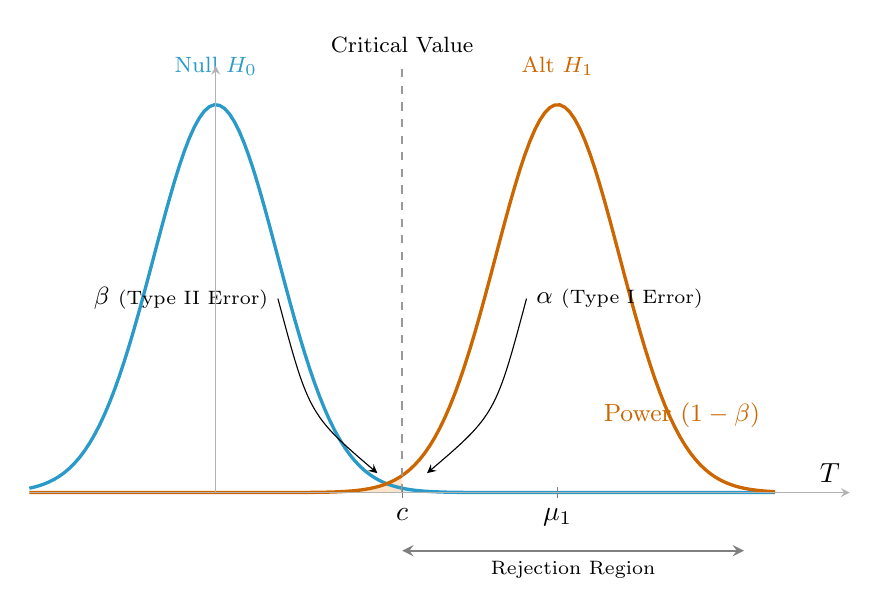
\begin{tikzpicture}[
    % Customizing the look for elegance
    declare function={norm(\x,\m,\s)=exp(-(\x-\m)^2/(2*\s^2));},
    >=stealth
]
\begin{axis}[
    width=12cm, height=7cm,
    axis lines=middle,
    inner axis line style={->, color=gray!60},
    xlabel={$T$}, ylabel={},
    domain=-3:9, samples=150,
    ytick=\empty,
    xtick={0, 3, 5.5},
    xticklabels={$\mu_0$, $c$, $\mu_1$},
    enlargelimits=upper,
    clip=false,
    axis on top % Ensures lines sit nicely on top of shading
]

    % --- 1. Shading Areas (The "Elegance" factor: Opacity and Pastel colors) ---
    
    % Alpha: Area under H0 to the right of c
    \addplot [fill=cyan!20, draw=none, domain=3:8] {norm(x,0,1)} \closedcycle;
    
    % Beta: Area under H1 to the left of c
    \addplot [fill=orange!20, draw=none, domain=-1:3] {norm(x,5.5,1)} \closedcycle;

    % --- 2. Plotting the Curves ---
    
    % H0 Distribution
    \addplot [very thick, cyan!80!black] {norm(x,0,1)};
    \node[cyan!80!black] at (axis cs: 0, 1.1) {\footnotesize Null $H_0$};

    % H1 Distribution
    \addplot [very thick, orange!80!black] {norm(x,5.5,1)};
    \node[orange!80!black] at (axis cs: 5.5, 1.1) {\footnotesize Alt $H_1$};

    % --- 3. Decision Boundary ---
    \draw [thick, gray!80, dashed] (axis cs:3,0) -- (axis cs:3,1.1) 
        node[pos=1.05, black] {\footnotesize Critical Value};

    % --- 4. Refined Labeling with Pointers ---
    
    % Alpha Label
    \draw[<-] (axis cs:3.4, 0.05) .. controls (axis cs:4.5, 0.2) .. (axis cs:5, 0.5) 
        node[right, font=\small] {$\alpha$ \scriptsize (Type I Error)};
        
    % Beta Label
    \draw[<-] (axis cs:2.6, 0.05) .. controls (axis cs:1.5, 0.2) .. (axis cs:1, 0.5) 
        node[left, font=\small] {$\beta$ \scriptsize (Type II Error)};
        
    % Power Label
    \node[orange!80!black] at (axis cs: 7.5, 0.2) {\small Power $(1-\beta)$};

    % Rejection Region Indicator
    \draw[thick, <->, gray] (axis cs:3, -0.15) -- (axis cs:8.5, -0.15) 
        node[midway, below, black] {\scriptsize Rejection Region};

\end{axis}
\end{tikzpicture}
\caption{Distribution overlap illustrating Type I and Type II errors.}
\end{figure}
   








\subsubsection{The Neyman-Pearson Proposal}
\vspace{-15pt}
The core philosophy of this approach is to treat Type I and Type II errors asymmetrically. We fix the maximum allowable probability of a Type I error ($\alpha$) and then attempt to minimize the Type II error (or equivalently, maximize the Power).

\begin{definition}
A test has a level of significance $\alpha$ if the probability of rejecting $H_0$ when it is true never exceeds $\alpha$ for any $\theta \in \Omega_0$.
\end{definition}

\begin{definition}
The size of the test is the "tightest" possible level, defined as the supremum of the power function over the null parameter space:$$\text{Size} = \sup_{\theta \in \Omega_0} \pi(\theta).$$
\end{definition}







\section{The Simple Likelihood Ratio and Most Powerful Tests}
\vspace{-15pt}
When both the null and alternative hypotheses are simple, we are essentially choosing between two fully specified probability distributions.

\begin{definition}[\textbf{Simple Likelihood Ratio Test}]
Let $X_1, X_2, \dots, X_n$ be a random sample from a distribution $f(x; \theta)$. To test $H_0: \theta = \theta_0$ vs $H_1: \theta = \theta_1$, we define the likelihood ratio as:$$\lambda(x) = \frac{L(\theta_0; x)}{L(\theta_1; x)} = \frac{\prod_{i=1}^n f(x_i; \theta_0)}{\prod_{i=1}^n f(x_i; \theta_1)}$$
The decision rule is:
\begin{itemize}
\item Reject $H_0$ if $\lambda(x) < k$
\item Fail to Reject $H_0$ if $\lambda(x) > k$
\item Randomize if $\lambda(x) = k$ (used primarily in discrete cases to achieve an exact size $\alpha$).
\end{itemize}
\end{definition}





\begin{remark}
\textbf{ }
\begin{enumerate}
\item If $H_0$ is true, $L(\theta_0)$ should be larger than $L(\theta_1)$, making $\lambda(x) > 1$.
\item If $H_1$ is true, $L(\theta_1)$ should be larger, making $\lambda(x) < 1$.
\item Therefore, ``small" values of $\lambda(x)$ provide evidence against $H_0$.
\end{enumerate}
\end{remark}




\begin{definition}[\textbf{Most Powerful (MP) Test}]
A test $\phi^*$ of $\, H_0: \theta = \theta_0$ versus $H_1: \theta = \theta_1$ is a most powerful test of size $\alpha \, (0 < \alpha < 1)$ if 
\begin{enumerate}
\item It has exactly $\alpha$:\,  $\pi_{\phi^*}(\theta_0) = \alpha$
\item For any other test $\phi$ with size $\leq \alpha$, the power of $\phi^*$ is at least as large: $\pi_{\phi^*}(\theta_1) \geq \pi_{\phi}(\theta_1)$.
%\item $\pi_{\phi^*}(\theta_1) \geq \pi_{\phi}(\theta_1)$, for any other test $\phi$ with $\pi_{\phi}(\theta_0) \leq \alpha$.
\end{enumerate}
i.e. a test $\phi^*$ is MP of size $\alpha$ if it has size $\alpha$, and if, among all other tests of size $\alpha$, ie has the largest power.
\end{definition}



\begin{lem}[\textbf{Neyman-Pearson Lemma}]
Let $X$ have probability density function $f(x;\theta), \, \theta \in \Omega$. Consider testing a simple null hypotheses $H_0: \theta = \theta_0$ against a simple alternative $H_1: \theta = \theta_1$. For a constant $k$, suppose the critical region defined by \[R = \left\{x:\quad \frac{f(x;\theta_1)}{f(x;\theta_0)}> k\right\}\] corresponds to a test of size $\alpha$. Then the test with this critical region is a most powerful test of size $\alpha$ for testing $H_0: \theta = \theta_0$ against $H_1: \theta = \theta_1$.
\end{lem}


\begin{proof}
Consider any other critical region $R_1$ with small size.

We need to show that \[P_{\theta_1}(X\in R) \geq P_{\theta_1}(X\in R_1)\] now
\[P_{\theta_0}(X\in R) = P_{\theta_0}(X\in R_1) = \alpha \]
\[\int_Rf(x;\theta_0)\, dx = \int_{R_1}f(x;\theta_0) \, dx\]
this implies
\[\int_{R\cap R_1}f(x;\theta_0)\, dx + \int_{R\cap R^c_1}f(x;\theta_0)\, dx = \int_{R_1\cap R}f(x;\theta_0)\, dx + \int_{R_1\cap R^c}f(x;\theta_0)\, dx\]
\begin{equation}
\implies\quad\int_{R\cap R_1^c}f(x;\theta_0)\, dx = \int_{R_1\cap R^c}f(x;\theta_0)\, dx
\end{equation}
for $x\in R\cap R^c_1$ \[\frac{f(x;\theta_1)}{f(x;\theta_0)} > k\quad\implies\quad f(x;\theta_1) > k\, f(x;\theta_0)\]
so that
\begin{equation}
\int_{R\cap R^c_1}f(x;\theta_1)\, dx > k\, \int_{R\cap R^c_1}f(x;\theta_0)\, dx
\end{equation}

for $x\in R_1 \cap R^c$
\[\frac{f(x;\theta_1)}{f(x;\theta_0)} < k\]
\[f(x;\theta_1) < k f(x;\theta_0)\]
\[-f(x;\theta_1) > -k \, f(x;\theta_0)\]
this implies
\begin{equation}
-\int_{R_1\cap R^c}f(x;\theta_1)\, dx  > -k \int_{R_1\cap R^c} f(x;\theta_0)\, dx
\end{equation}
now
\begin{align*}
P_{\theta_1}(X\in R) & = \int_{R}f(x;\theta_1)\, dx\\
& = \int_{R\cap R_1}f(x;\theta_1)\, dx + \int_{R\cap R^c_1}f(x;\theta_1)\, dx
\end{align*}

\begin{align*}
P_{\theta_1}(X \in R_1) & = \int_{R_1} f(x;\theta_1)\, dx\\
& = \int_{R_1\cap R}f(x;\theta_1)\, dx + \int_{R_1\cap R^c}f(x;\theta_1)\, dx
\end{align*}

\begin{align*}
P_{\theta_1}(X\in R) - P_{\theta_1}(X\in R_1) & = \int_{R\cap R^c_1}f(x;\theta_1)\, dx - \int_{R_1\cap R^c}f(x;\theta_1)\, dx\\
& \geq k\int_{R\cap R^c_1}f(x;\theta_0)\, dx - k\int_{R_1\cap R^c}f(x;\theta_0)\, dx \quad (\text{by 3.2 and 3.3})\\
& = k\underbrace{\left[\int_{R\cap R^c_1} f(x;\theta_0)\, dx - \int_{R_1\cap R^c}f(x;\theta_0)\, dx\right]}_{0 \quad \text{by 3.1}}\\
& = 0.
\end{align*}
Therefore, $P_{\theta_1}(X\in R) - P_{\theta_1}(X\in R_1)\geq 0\,$ or $\, P_{\theta_1}(X\in R) \geq P_{\theta_1}(X\in R_1)$.
\end{proof}



\begin{example}
Let $X_1, X_2, \cdots , X_n$ be a random sample from $X\thicksim N(\mu,16)$. Find the most powerful test of size $\alpha = 0.05$ of
\begin{enumerate}
\item[ ] $H_0: \mu = 10$
\item [ ] $H_1: \mu  = 12$.
\end{enumerate}
\end{example}

\begin{proof}[\textit{Solution}.]
According to the Neyman-Pearson Lemma, the MP test rejects $H_0$ when 
$$\frac{\prod^n_{i = 1} f(x_i; \theta_1)}{\prod^n_{i = 1}f(x_i;\theta_0)} > k.$$
\[\frac{\prod^n_{i = 1}\frac{1}{\sqrt{2\pi (16)}}e^{-\frac{1}{2(16)}(x_i - 12)^2}}{\prod^n_{i = 1}\frac{1}{\sqrt{2\pi (16)}}e^{-\frac{1}{2(16)}(x_i - 10)^2}} > k\]

\[\frac{(32\pi)^{-\frac{n}{2}}e^{-\frac{1}{32}\sum^n_{i = 1}(x_i - 12)^2}}{(32\pi)^{-\frac{n}{2}}e^{-\frac{1}{32}\sum^n_{i = 1}(x_i - 10)^2}} > k\]

\[\implies \quad e^{-\frac{1}{32}\sum^n_{i=1}(x_i - 12)^2+ \frac{1}{32}\sum^n_{i = 1}(x_i - 10)^2}\, > k\]
\[-\frac{1}{32}\sum^n_{i=1}(x_i - 12)^2+ \frac{1}{32}\sum^n_{i = 1}(x_i - 10)^2\, >\ln k\]
\[\frac{1}{32}\left[\sum^n_{i=1}(x_i^2 - 20x_i +  100)- \sum^n_{i = 1}(x_i^2 - 24x_i + 144)\right]\, > k_1\]
\[\implies \quad \sum^n_{i = 1}\left(x^2_i - 20x_i + 100 - x^2_i + 24x_i - 144\right) \, > \, k_1(32)\]
\[\sum^n_{i = 1}\left(-44 + 4x_i\right) > k_2\]
\[-44n + 4\sum^n_{i = 1} x_i > k_2\]
\[4\sum^n_{i = 1} x_i > k_2 + 44n\]
\[4\sum^n_{i = 1} x_i > k_3\]
\[\sum^n_{i = 1} x_i > \frac{k_3}{4} = k_4\]
\[\overline{x} > \frac{k_4}{n}\]
\[\implies\quad \overline{x} > c\]
i.e. $\, R = \{(x_1, \cdots, x_n)\, |\, \overline{x} > c\}\,$ for some $c$ 
\[P_{H_0}\left(\overline{X} > c\right) = 0.05\]
\[P\left(\frac{\overline{X} - \mu_0}{\frac{\sigma}{\sqrt{n}}} > \frac{c - \mu_0}{\frac{\sigma}{\sqrt{n}}}\right) = 0.05\]
\[P\left(Z > \frac{c - 10}{\frac{4}{\sqrt{n}}}\right) = 0.05\]
\[\frac{c - 10}{\frac{4}{\sqrt{n}}} = Z_{0.05}\]
Using the standard normal table, $P(Z > 1.645) = 0.05$. Therefore:
\[\implies\quad c = 10 + 1.645\, \frac{4}{\sqrt{n}}.\]

Therefore, $$R = \left\{(x_1, \cdots, x_n)\, |\, \overline{x} > 10 +  \frac{6.58}{\sqrt{n}}\right\}$$ is the critical region of a MP test of $H_0: \mu = 10$ versus $H_1: \mu = 10$.
\end{proof}

Additionally, ($\alpha=0.05, \mu_0=10, \sigma=4$), the power function for a sample of size $n$ is:$$\pi(\mu) = P_{\mu}(\bar{X} > c) = 1 - \Phi\left( \frac{c - \mu}{4/\sqrt{n}} \right)$$where $c = 10 + 6.58/\sqrt{n}$.

\begin{figure}[H]
\centering
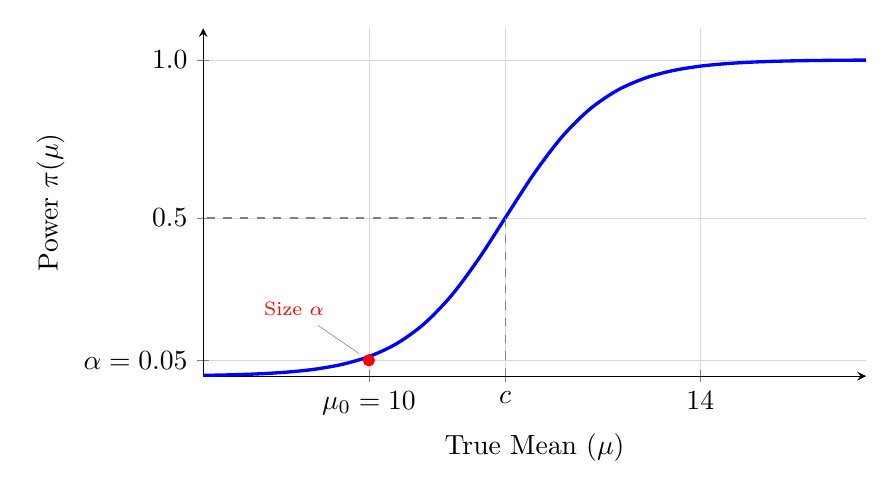
\begin{tikzpicture}[
    declare function={
        % Standard Normal CDF approximation
        Phi(\x)=1/(1+exp(-1.6545*\x));
        % Power function for our specific example (n=16)
        % c = 10 + 1.645 * (4/sqrt(16)) = 11.645
        % std_error = 4/sqrt(16) = 1
        power(\mu)=1 - Phi(11.645 - \mu);
    }
]
\begin{axis}[
    width=10cm, height=6cm,
    xlabel={True Mean ($\mu$)},
    ylabel={Power $\pi(\mu)$},
    ymin=0, ymax=1.1,
    xmin=8, xmax=16,
    grid=both,
    grid style={line width=.1pt, draw=gray!10},
    major grid style={line width=.2pt, draw=gray!30},
    axis lines=left,
    xtick={10, 11.645, 14},
    xticklabels={$\mu_0=10$, $c$, 14},
    ytick={0.05, 0.5, 1.0},
    yticklabels={$\alpha=0.05$, 0.5, 1.0}
]
    % Plot the power curve
    \addplot[very thick, blue, smooth, domain=8:16] {power(x)};
    
    % Highlight the alpha point
    \addplot[only marks, mark=*, red] coordinates {(10, 0.05)} 
        node[pin=135:{\scriptsize Size $\alpha$}] {};

    % Dashed line for Power = 0.5 at mu = c
    \draw[dashed, gray] (axis cs:11.645, 0) -- (axis cs:11.645, 0.5) -- (axis cs:8, 0.5);

\end{axis}
\end{tikzpicture}
\caption{Power Curve for $H_0: \mu = 10$ with $n=16$. Note that power is $\alpha$ at the null and increases as $\mu$ increases.}
\end{figure}



\begin{exe}
Let $X_1, X_2, \cdots , X_n$ be a random sample from $X\thicksim N(\mu, \sigma^2)$ with $\sigma^2$ known. Find the most powerful test of size $\alpha$ of $\, H_0:\, \mu = \mu_0\, $ against $\, H_1: \, \mu = \mu_1$ (where $\mu_1 > \mu_0$).
\end{exe}














\begin{example}
Let $X_1,  X_2, \cdots , X_n$ be a random sample from $N(\mu, \sigma^2)$ with $\mu$ known. Find the most powerful test of size $\alpha$. of $H_0: \sigma = \sigma_0$ versus $H_1: \sigma = \sigma_1$ (where $\sigma_1 < \sigma_0)$.
\end{example}


\begin{proof}[\textit{Solution.}]
According to the Neyman-Pearson Lemma, the MP test rejects $H_0$ when
\[\frac{\prod^n_{i = 1} f(x_i;\theta_1)}{\prod^n_{i = 1} f(x_i; \theta_0)} > k.\]
\[\frac{\prod^n_{i = 1}\frac{1}{\sqrt{2\pi \sigma^2_1}}e^{-\frac{1}{2\sigma^2_1}(x_i -\mu)^2}}{\prod^n_{i = 1}\frac{1}{\sqrt{2\pi \sigma^2_0}}e^{-\frac{1}{2\sigma^2_0}(x_i -\mu)^2}} > k\]
\[\frac{(2\pi \sigma^2_1)^{-\frac{n}{2}}     e^{-\frac{1}{2\sigma^2_1}\sum^n_{i = 1}(x_i -\mu)^2}}{(2\pi \sigma^2_0)^{-\frac{n}{2}}     e^{-\frac{1}{2\sigma^2_0}\sum^n_{i = 1}(x_i -\mu)^2}} > k\]
\[\left(\frac{2\pi\sigma^2_0}{2\pi\sigma^2_1}\right)^{\frac{n}{2}}e^{\frac{1}{2\sigma^2_0}\sum^n_{i = 1}(x_i -\mu)^2 - \frac{1}{2\sigma^2_1}\sum^n_{i =1}(x_i - \mu)^2} > k\]
\[e^{\left(\frac{1}{2\sigma^2_0}-\frac{1}{2\sigma^2_1}\right)\sum^n_{i = 1} (x_i - \mu)^2}> k_1\]
\[\frac{1}{2}\left(\frac{1}{\sigma^2_0}-\frac{1}{\sigma^2_1}\right)\sum^n_{i = 1} (x_i - \mu)^2> k_2\]
\[\sum^n_{i = 1}(x_i - \mu)^2 < \frac{k_2}{\frac{1}{2}\left(\frac{1}{\sigma^2_0}-\frac{1}{\sigma^2_1}\right)}\]
\[\implies\quad \sum^n_{i = 1} (x_i - \mu)^2 < c\]

i.e. $\, R = \left\{(x_1,\cdots , x_n)\, |\, \sum^n_{i = 1}(x_i - \mu)^2 < c\right\}$

Now
\[P_{H_0}\left(\sum^n_{i = 1}(X_i - \mu)^2 < c\right) = \alpha\]
\[P\left(\sum^n_{i = 1} \left(\frac{X_i- \mu}{\sigma_0}\right)^2 < \frac{c}{\sigma_0^2}\right) = \alpha\]
\[P\left(\chi^2_n < \frac{c}{\sigma^2_0}\right) = \alpha\]
that is \[\frac{c}{\sigma^2_0} = \chi^2_{n,1-\alpha} \quad\implies\quad c = \sigma^2_0\, \chi^2_{n,1-\alpha}.\]
Therefore \[R = \left\{(x_1, \cdots, x_n)\, |\, \sum^n_{i = 1}(X_i - \mu)^2 < \sigma^2_0\, \chi^2_{n,1-\alpha}\right\}\] is the critical region of a MP test of $H_0: \sigma = \sigma_0$ versus $H_1: \sigma = \sigma_1 \, (\sigma_1 < \sigma_0)$.
\end{proof}



\begin{example}
Let $X_1,X_2,\cdots,X_n$ be a random sample from exponential $$f_X(x,\lambda)=\frac{1}{\theta}e^{-\frac{x}{\theta}},\quad \lambda >0,\quad x>0$$
Find the most powerful test for testing $\, H_0:\theta =\theta_0\,$ against $\,H_1:\theta =\theta_1$ where $\theta_0>\theta_1$
\end{example}

\begin{proof}[\textbf{\textit{Solution}}]
According to the Neyman-Pearson Lemma, the MP test rejects $H_0$ when 
\[\frac{\prod^n_{i = 1}f(x_i;\theta_1)}{\prod^n_{i = 1}f(x_i;\theta_0)} > k.\]
\[\frac{\theta^{-n}_1e^{-\frac{1}{\theta_1}\sum^n_{i = 1} x_i}}{\theta^{-n}_0e^{{-\frac{1}{\theta_0}}\sum^n_{i = 1} x_i}} > k\]
\[\left(\frac{\theta_0}{\theta_1}\right)^ne^{{-\left(\frac{1}{\theta_1}-\frac{1}{\theta_0}\right)}\sum^n_{i = 1}x_i} > k\]
\[n[\ln(\theta_0)-\ln(\theta_1)] - \left(\frac{1}{\theta_1}-\frac{1}{\theta_0}\right)\sum^n_{i = 1} x_i > k_1\]
\[- \left(\frac{1}{\theta_1}-\frac{1}{\theta_0}\right)\sum^n_{i = 1} x_i > k_2= k_1 +n[\ln(\theta_0) - \ln(\theta_1)]\]
We are given that $\theta_0 > \theta_1$. This implies:$$\frac{1}{\theta_1} > \frac{1}{\theta_0} \implies \left(\frac{1}{\theta_1} - \frac{1}{\theta_0}\right) > 0.$$
Therefore 
$$\sum_{i=1}^n x_i < \frac{k_2}{-\left(\frac{1}{\theta_1} - \frac{1}{\theta_0}\right)}$$$$\sum_{i=1}^n x_i < c$$ The critical region is therefore $R = \{ (x_1, \dots, x_n) | \sum_{i=1}^n x_i < c \}$.

Now, to find $c$, we need the distribution of $Y = \sum^n_{i = 1} X_i$. Recall that if $X_i \sim \text{Exp}(\theta)$, then $\sum X_i \sim \text{Gamma}(n, \theta)$. Furthermore, it is a standard result that $\frac{2\sum^n_{i = 1} X_i}{\theta} \sim \chi^2_{2n}$.
$$P_{H_0}(\sum X_i < c) = \alpha$$
Standardize to the Chi-square distribution by multiplying by $\frac{2}{\theta_0}$: $$P\left( \frac{2\sum X_i}{\theta_0} < \frac{2c}{\theta_0} \right) = \alpha$$$$P(\chi^2_{2n} < \frac{2c}{\theta_0}) = \alpha$$
Using the notation $\chi^2_{2n, 1-\alpha}$ for the value that leaves $\alpha$ in the lower tail:$$\frac{2c}{\theta_0} = \chi^2_{2n, 1-\alpha} \implies c = \frac{\theta_0}{2} \chi^2_{2n, 1-\alpha}$$ The Most Powerful test of size $\alpha$ rejects $H_0$ if:$$\sum_{i=1}^n x_i < \frac{\theta_0}{2} \chi^2_{2n, 1-\alpha}$$
The critical region is therefore $$R = \left\{ (x_1, \dots, x_n) |  \sum_{i=1}^n x_i < \frac{\theta_0}{2} \chi^2_{2n, 1-\alpha}\right\}.$$
\end{proof}





\begin{note}
For a given $\alpha$, it is not always possible to find a value $c$ such that this is true. e.g. Let $n = 3, \quad \theta_0 = \frac{3}{4}, \quad \theta_1 = \frac{1}{4}, \quad \alpha = 0.05.\quad$ Then $\, \operatorname{BIN}(3,\frac{3}{4})$ has distribution.
\begin{table}[H]
\centering
\begin{tabular}{c|cccc}
$y$ & 0 & 1 & 2 & 3\\
\hline
$P(Y = y)$ & 0.0156 & 0.1406 & 0.4219 & 0.4219
\end{tabular}
\end{table}
i.e
\[P(Y = 2) = \binom{3}{2}\left(\frac{3}{4}\right)^2\left(\frac{1}{4}\right) = 0.4219\]
Then, if
\begin{align*}
c = 0, & \quad P_{\theta_0}(Y \leq c) = P(Y = 0) = 0.0156\, < \, 0.05\\
c = 1, & \quad P_{\theta_0}(Y\leq c) = P(Y = 0) + P(Y = 1) = 0.1562\, > 0.05
\end{align*}

In discrete cases, the ``jump" in cumulative probability can skip over the desired $\alpha$. As shown in the example with $Y \sim \text{Bin}(3, 0.75)$: If we reject only at $y=0$, our size is $0.0156$ (too conservative). If we reject at $y=0$ and $y=1$, our size jumps to $0.1562$ (exceeds $\alpha = 0.05$). To fix this, we use a \textit{Randomized Test}, where if the test statistic hits the boundary value, we reject $H_0$ with a specific probability $p$. This allows us to hit exactly $\alpha = 0.05$ on average.
\end{note}








%%%%
\section{Composite Hypotheses}
\vspace{-15pt}
When the hypotheses are composite (e.g., $H_0: \theta \leq \theta_0$), we can no longer use the simple Neyman-Pearson ratio because $\theta$ is not a single value. Instead, we use the Likelihood Ratio Test (LRT).



For a more general testing problem \[H_0: \theta \in \Omega_0\quad \text{versus}\quad H_1:\theta \in \Omega_1\] where $\Omega_0$ and $\Omega_1$ contain more than one point, we could either consider the ratio \[\frac{\sup_{\theta \in \Omega_1} L(\theta; x)}{\sup_{\theta \in \Omega_0}L(\theta;x)}\] or \[\frac{\sup_{\theta \in \Omega} L(\theta; x)}{\sup_{\theta \in \Omega_0}L(\theta;x)}= \Lambda(x)\] and reject $H_0$ if $\Lambda(x)$ is too large.



\begin{definition}
The generalized likelihood ratio function for a null hypothesis $H_0: \theta \in \Omega_0$ against $H_1: \theta \in \Omega_1\, (\Omega - \Omega_0)$ is defined by \[\Lambda(x) = \Lambda(x_1, \cdots , x_n) = \frac{\sup_{\theta \in \Omega} L(\theta; x)}{\sup_{\theta \in \Omega_0}L(\theta;x)}.\]
The corresponding statistic \[\Lambda(X) = \Lambda(X_1, \cdots , X_n)\] is called the generalized likelihood ratio statistic.
\end{definition}

\begin{note}\textbf{ }
\begin{enumerate}
\item $\sup_{\theta \in \Omega}L(\theta;x)$ is maximized over the entire sample space (unrestricted maximization) thus \[\sup_{\theta \in \Omega} L(\theta;x) = L(\hat{\theta};x)\] where $\hat{\theta}$ is the ML-estimate of $\theta$.
\item $\sup_{\theta \in \Omega_0} L(\theta;x)$ is maximized over $\Omega_0$ (restricted maximization) thus \[\sup_{\theta \in \Omega_0}L(\theta;x) = L(\hat{\theta}_R;x)\] where $\hat{\theta}_R$ is the M.L. estimate obtained under the restriction $H_0: \theta \in \Omega_0$.
\item Thus $\Lambda(x)$ can also be expressed as \[\Lambda(x) = \frac{L(\hat{\theta};x)}{L(\hat{\theta}_R;x)}.\]
\item The critical region of this test has the form \[R = \left\{(x_1, \cdots , x_n)\, |\, \Lambda(x_1, \cdots, x_n)\, > \, c\right\}\]
where $c$ is determined by the size of the test. i.e \[P_{H_0}(X\in R) = \alpha\]
\[\sup_{\theta \in \Omega_0}P\left(\Lambda(X) > c\right) = \alpha.\]
In general the distribution of $\Lambda(X)$ may be difficult to find, thus an asymptotic chi-square distribution is often used.
\end{enumerate}
\end{note}



\begin{example}
Let $X_1, X_2, \cdots , X_n$ be a random sample from $X\thicksim N(\mu, \sigma^2)$, where $\sigma^2$ is known. Find the generalized likelihood ratio test of the hypothesis $H_0: \, \mu = \mu_0$ against $H_1:\, \mu \neq \mu_0$.
\end{example}

\begin{proof}[\textbf{\textit{Solution}}]
$f(x;\mu) = \frac{1}{\sqrt{2\pi \sigma^2}} e^{-\frac{1}{2\sigma^2}(x_i - \mu)^2}\, ,$\quad $\Omega = \mathbb{R}, \quad \Omega_0 = \{\mu_0\}$
\[\Lambda(x) = \frac{L(\hat{\theta}; x)}{L(\hat{\theta}_R;x)} = \frac{L(\hat{\mu};x)}{L(\mu_0;x)}\]
\[L(\mu;x) = \prod^n_{i = 1}\frac{1}{\sqrt{2\pi \sigma^2}} e^{-\frac{1}{2\sigma^2}(x_i - \mu)^2}=(2\pi\sigma^2)^{-\frac{n}{2}} e^{-\frac{1}{2\sigma^2}\sum^n_{i = 1}(x_i - \mu)^2}\]
\[l(\mu) = -\frac{n}{2}\ln 2\pi \sigma^2 - \frac{1}{2\sigma^2}\sum^n_{i = 1} (x_i -\mu)^2\]
\[\frac{\partial l}{\partial \mu} = -\frac{1}{2\sigma^2}(-2)\sum^n_{i = 1}(x_i - \mu)\]
\[\frac{\partial l}{\partial \mu} = 0\quad \implies \quad \sum^n_{i = 1}(x_i  - \mu) = 0 \]
\[\therefore\,\hat{\mu} = \overline{x}\]
Therefore 
\[L(\hat{\theta};x) = (2\pi\sigma^2)^{-\frac{n}{2}}e^{-\frac{1}{2\sigma^2}\sum^n_{i = 1}(x_i - \overline{x})^2}.\]
Under $H_0:\, \mu = \mu_0$
\[L(\hat{\theta}_R;x) = (2\pi\sigma^2)^{-\frac{n}{2}}e^{-\frac{1}{2\sigma^2}\sum^n_{i = 1}(x_i - \mu_0)^2}\]
Therefore
\[\Lambda(x) = \frac{(2\pi\sigma^2)^{-\frac{n}{2}}e^{-\frac{1}{2\sigma^2}\sum^n_{i = 1}(x_i - \overline{x})^2}}{(2\pi\sigma^2)^{-\frac{n}{2}}e^{-\frac{1}{2\sigma^2}\sum^n_{i = 1}(x_i - \mu_0)^2}}\, > \, k\]
\[\implies\, e^{\frac{1}{2\sigma^2}\sum^n_{i = 1}(x_i - \mu_0)^2 - \frac{1}{2\sigma^2}\sum^n_{i = 1}(x_i - \overline{x})^2} > k\]
\[\frac{1}{2\sigma^2}\sum^n_{i = 1}\left[x^2_i - 2\mu_0x_i + \mu^2_0 - (x_i^2 - 2\overline{x}x_i + \overline{x}^2)\right] > k_1\]
\[\frac{1}{2\sigma^2}\sum^n_{i = 1}\left[-2\mu_0x_i + \mu_0^2 + 2\overline{x}x_i - \overline{x}^2\right] > k_1\]
\[\frac{1}{2\sigma^2}\left[-2n\mu_0\overline{x} + n\mu_0^2+2n\overline{x}^2 - \overline{x}^2\right] > k_1\]
\[\frac{1}{2\sigma^2}\left[n\overline{x}^2-2n\mu_0\overline{x} + n\mu^2_0\right] > k_1\]
\[\frac{n}{2\sigma^2}(\overline{x}-\mu_0)^2 > k_1\]
\[\frac{n}{\sigma^2}(\overline{x}-\mu_0)^2 > k_2\]
\[\implies\quad \left(\frac{\overline{x}-\mu_0}{\frac{\sigma}{\sqrt{n}}}\right)^2 > k_2\]
\[\left|\frac{\overline{x} - \mu_0}{\frac{\sigma}{\sqrt{n}}}\right| > c\]
i.e 
\[R = \left\{(x_1, \cdots, x_n)\, \Big|\, \left|\frac{\overline{x} - \mu_0}{\frac{\sigma}{\sqrt{n}}}\right| > c\right\}\]
is the rejection region, where $c$ is determined by the size of the test $\alpha$.
\[P_{H_0}(X\in R) = \alpha\]
\[P\left(\left|\frac{\overline{X} - \mu_0}{\frac{\sigma}{\sqrt{n}}}\right|> c\right) = \alpha\]
\[P(|Z| > c) = \alpha\]
$$c  = Z_{\frac{\alpha}{2}}$$
Therefore
\[R = \left\{(x_1, \cdots, x_n)\, \Big|\, \left|\frac{\overline{x} - \mu_0}{\frac{\sigma}{\sqrt{n}}}\right| > Z_{\frac{\alpha}{2}}\right\}\] is the critical region of the generalized likelihood ratio test of size $\alpha$ of $H_0: \mu = \mu_0$ against $H_1:\, \mu\neq \mu_0$.
\end{proof}






\begin{example}
Let $X_1, X_2, \cdots, X_n$ be a random sample from the $N(\mu,\sigma^2)$ distribution where $\mu$ and $\sigma^2$ are unknown. Consider a test of $H_0: \mu = 0$ against $H_1: \mu \neq 0$.
\begin{enumerate}
\item[(i).] Show that the generalized likelihood ratio test of $H_0$ against $H_1$ has critical region \[R = \left\{(x_1, \cdots, x_n) \, \Big| \, \frac{n\overline{x}^2}{s^2} > c\right\}.\]
\begin{proof}[\textbf{\textit{Solution}}]
$\Omega = \{(\mu, \sigma^2)| -\infty < \mu < \infty,  \sigma^2>0\}$ \, and \, $\Omega_0= \{(\mu, \sigma^2) |\mu = 0, \sigma^2 > 0\}$
\[\Lambda(x)  = \frac{L(\hat{\theta}; x)}{L(\hat{\theta}_R; x)} \quad \text{where}\quad \theta = (\mu, \sigma^2)\]
\[L(\theta;x) = \prod^n_{i = 1}\frac{1}{\sqrt{2\pi\sigma^2}}e^{-\frac{1}{2\sigma^2}\sum^n_{i = 1} (x_i - \mu)^2} = (2\pi\sigma^2)^{-\frac{n}{2}}\, e^{-\frac{1}{2\sigma^2} (x_i - \mu)^2}\]
\[l(\theta) = -\frac{n}{2}\ln(2\pi\sigma^2) - \frac{1}{2\sigma^2}\sum^n_{i = 1}(x_i - \mu)^2\]

\[S(\theta) = \begin{pmatrix}
\frac{\partial l}{\partial \mu}\\
\frac{\partial l}{\partial \sigma^2}\\
\end{pmatrix}\]
\[\frac{\partial l}{\partial \mu} = -\frac{1}{2\sigma^2}(-2)\sum^n_{i = 1}(x_i -\mu) = \frac{1}{\sigma^2}\sum^n_{i = 1}(x_i -\mu).\]
$\frac{\partial l}{\partial \mu} = 0$
\[\implies\quad \sum^n_{i = 1} x_i - n\mu = 0\]
\[\therefore\quad \hat{\mu} = \overline{x}.\]

\[\frac{\partial l}{\partial \sigma^2} = -\frac{n}{2}\cdot\frac{2\pi}{2\pi\sigma^2} + \frac{1}{2(\sigma^2)^2}\sum^n_{i =1}(x_i - \mu)^2 = -\frac{n}{2\sigma^2}+ \frac{1}{2(\sigma^2)^2}\sum^n_{i = 1}(x_i - \mu)^2.\]
$\frac{\partial l}{\partial \sigma^2} = 0$
\[\implies \quad\hat{\sigma}^2 = \frac{1}{n}\sum^n_{i = 1}(x_i - \mu)^2\]
Therefore
\begin{align*}
L(\hat{\theta}) & = L(\hat{\mu}, \hat{\sigma}^2)\\
& = (2\pi \hat{\sigma}^2)^{-\frac{n}{2}}e^{-\frac{1}{2\hat{\sigma}^2}\sum^n_{i = 1}(x_i - \hat{\mu})^2}\\
& = (2\pi \hat{\sigma}^2)^{-\frac{n}{2}}e^{-\frac{1}{2\hat{\sigma}^2}\sum^n_{i = 1}(x_i - \overline{x})^2}\\
& = \left(\frac{2\pi}{n}\sum^n_{i = 1} (x_i - \overline{x})^2\right)^{-\frac{n}{2}}e^{-\frac{n}{2}}
\end{align*}
Under $H_0$:
\[L(\theta_R;x) = \prod^n_{i = 1}\frac{1}{\sqrt{2\pi \sigma^2}}e^{-\frac{1}{2\sigma^2}x_i^2}\]
\[L(\theta)  = (2\pi \sigma^2)^{-\frac{n}{2}}e^{-\frac{1}{2\sigma^2}\sum^n_{i = 1} x_i^2}\]
\[l(\theta) = -\frac{n}{2}\ln (2\pi \sigma^2) - \frac{1}{2\sigma^2}\sum^n_{i = 1}x_i^2\]
\[S(\theta) = \frac{\partial l}{\partial \sigma^2}\]
\[\frac{\partial l}{\partial \sigma^2} = -\frac{n}{2}\cdot\frac{2\sigma}{2\sigma\, \sigma^2} + \frac{1}{2(\sigma^2)^2}\sum^n_{i = 1}x_i^2=-\frac{n}{2\sigma^2}+ \frac{1}{2(\sigma^2)^2}\sum^n_{i = 1} x_i^2\]
\[\frac{\partial l}{\partial \sigma^2} = 0\quad \implies\quad \hat{\sigma}^2_R = \frac{1}{n}\sum^n_{i = 1} x_i^2\]
Therefore
\begin{align*}
L(\hat{\theta}_R) & = L(\hat{\theta}^2_R)\\
& = (2\pi \hat{\theta}^2_R)^{-\frac{n}{2}}\, e^{-\frac{1}{2\hat{\sigma}^2_R}\sum^n_{i = 1}x_i^2}\\
& = \left(\frac{2\pi}{n}\sum^n_{i =  1} x_i^2\right)^{-\frac{n}{2}} e^{-\frac{n}{2}}.
\end{align*}
Therefore
\[\frac{L(\hat{\theta})}{L(\hat{\theta}_R)} > k\]
\[\frac{\left(\frac{2\pi}{n}\sum^n_{i = 1} (x_i - \overline{x})^2\right)^{-\frac{n}{2}}e^{-\frac{n}{2}}}{\left(\frac{2\pi}{n}\sum^n_{i = 1} x_i^2\right)^{-\frac{n}{2}}e^{-\frac{n}{2}}} > k\]
\[\left(\frac{\sum^n_{i = 1} (x_i - \overline{x})^2}{\sum^n_{i = 1} x_i^2}\right)^{-\frac{n}{2}} > k\]
\[\left(\frac{\sum^n_{i = 1}(x_i - \overline{x} + \overline{x})^2}{\sum^n_{i = 1}(x_i - \overline{x})^2}\right)^{\frac{n}{2}} > k\]
\[\left(\frac{\sum^n_{i = 1} \left[(x_i - \overline{x})^2 + 2\overline{x}(x_i - \overline{x})+ \overline{x}^2\right]}{\sum^n_{i = 1} (x_i - \overline{x})^2}\right)^{\frac{n}{2}} > k\]
\[\left(\frac{\sum^n_{i = 1} (x_i - \overline{x})^2 + n\overline{x^2}}{\sum^n_{i = 1}(x_i - \overline{x})^2}\right)^{\frac{n}{2}}\]
\[\implies \quad \left(1 + \frac{n\overline{x}^2}{\sum^n_{i = 1}(x_i - \overline{x})^2}\right)^{\frac{n}{2}} > k\]
\[\frac{n\overline{x}^2}{(n-1)S^2}> k_1\]
\[\frac{n\overline{x}^2}{S^2} > c\]
Therefore \[R = \left\{(x_1, \cdots, x_n)\, \Big|\, \frac{n\overline{x}^2}{S^2} > c\right\}.\]
\end{proof}


\item[(ii).] Show that the statistic  $T = \frac{n\overline{X}^2}{S^2}$ has a $F(1,n-1)$ distribution under $H_0$ and thus find a size $\alpha = 0.05$ test for $n = 20$.
\begin{proof}[\textit{Solution.}]
\begin{align*}
T  & = \frac{n\overline{X}^2}{S^2}
 = \frac{n\left(\frac{\overline{X}-0}{\sigma}\right)^2}{\frac{S^2}{\sigma^2}}
 = \frac{\left(\frac{\overline{X}-0}{\frac{\sigma}{\sqrt{n}}}\right)^2}{\frac{(n-1)\frac{S^2}{\sigma^2}}{n-1}}
\end{align*}
\[\frac{\overline{X} - 0}{\frac{\sigma}{\sqrt{n}}}\, \thicksim\, N(0,1)\quad \implies\quad \left(\frac{\overline{X}-0}{\frac{\sigma}{\sqrt{n}}}\right)^2\, \thicksim\, \frac{\chi^2(1)}{1}\]

\[\frac{(n-1)S^2}{\sigma^2}\, \thicksim\, \chi^2(n-1)\]
\[\frac{(n-1)\frac{S^2}{\sigma^2}}{n-1}\, \thicksim \, \frac{\chi^2(n-1)}{n-1}\]
$\overline{X}$ and $S^2$ are independent.

Therefore, $\chi^2(1)$ and $\chi^2(n-1)$ are independent.
\[\therefore\quad \frac{n\, \overline{X}^2}{S^2}\, \thicksim \, F(1,n-1).\]
$P_{H_0}(X\in R) = \alpha$
\[P\left(\frac{n\overline{X}^2}{S^2} > c\right) = \alpha\]
\[P(F_{1,n-1} > c) = 0.05\]
\[P(F_{1,19} > c) = 0.05\]
$c = 4.35$

Therefore \[R = \left\{(x_1, \cdots, x_n)\, \Big|\, \frac{20\overline{x}^2}{S^2} > 4.35\right\}\] is the critical region.
\end{proof}
\end{enumerate}
\end{example}



\begin{note}
$\frac{(n - 1)\, S^2}{\sigma^2}\, \thicksim\, \chi^2(n-1)$ 

e.g Var$(S^2) = ??$
\begin{align*}
\operatorname{Var}(S^2) & = \operatorname{Var}\left[\frac{\sigma^2}{n - 1}\cdot\frac{(n-1)S^2}{\sigma^2}\right]\\
& = \frac{\sigma^4}{(n - 1)^2}\, \operatorname{Var}\left[\frac{(n - 1)S^2}{\sigma^2}\right]\\
& = \frac{\sigma^4}{(n - 1)^2}\, 2(n-1)\\
& = \frac{2\sigma^4}{n - 1}.
\end{align*}
\end{note}






\begin{example}
Let $X_1, X_2, \cdots, X_n$ and $Y_1, Y_2, \cdots, Y_m$ be two independent random samples from $$f(x;\theta) = \frac{1}{\theta}e^{-\frac{x}{\theta}}\, , \quad x >0$$ and $$f(y;\mu) = \frac{1}{\mu}e^{-\frac{x}{\mu}}\, , \quad y >0$$ respectively.
\begin{enumerate}
\item[(a).] Show that the generalized likelihood ratio for testing the hypothesis $H_0:\theta = \mu$ against $H_1: \theta \neq \mu$ is a function of the statistic $$T = \frac{\sum^n_{i = 1} X_i}{\sum^n_{i = 1} X_i + \sum^m_{i = j} Y_j}.$$
\begin{proof}[\textit{Solution}.]
$\Omega = \{(\theta,\mu):\, \theta > 0,\, \mu > 0\}\quad$ and $\quad \Omega_0 = \{(\theta,\mu):\, \theta = \mu\}$
\[\Lambda(x,y) = \frac{L(\hat{\theta})}{L(\hat{\theta}_R)}\]
\begin{align*}
L(\theta, \mu) & = \prod^n_{i = 1} f(x_i;\theta)\, \prod^m_{j = 1} f(y_j;\mu)\\
& = \prod^n_{i = 1} \frac{1}{\theta}\, e^{-\frac{x_i}{\theta}}\, \prod^m_{j=1}\frac{1}{\mu}\, e^{-\frac{y_j}{\mu}}\\
& = \theta^{-n}\, e^{-\frac{1}{\theta}\sum^n_{i =1} x_i}\, \mu^{-m}\, e^{-\frac{1}{\mu}\sum^m_{j=1}y_j}.
\end{align*}
\[l(\theta,\mu) = -n\ln\theta - \frac{1}{\theta}\sum^n_{i = 1} x_i - m\ln\mu - \frac{1}{\mu}\sum^m_{j = 1} y_j.\]

The score vector \[S(\theta,\mu) = \begin{pmatrix}
\frac{\partial l}{\partial\theta}\\
\frac{\partial l}{\partial \mu}\\
\end{pmatrix}\]

\[\frac{\partial l}{\partial \theta} = -\frac{n}{\theta} + \frac{1}{\theta^2}\, \sum^n_{i = 1} x_i\]
$\frac{\partial l}{\partial \theta}= 0$
\[\frac{n}{\theta} = \frac{1}{\theta^2}\, \sum^n_{i = 1} x_i\quad \implies\quad \hat{\theta} = \frac{1}{n}\sum^n_{i = 1} x_i = \overline{x}.\]
Similarly
\[\hat{\mu} = \frac{1}{m}\, \sum^m_{j = 1} y_j = \overline{y}.\]

\begin{align*}
L(\hat{\theta}) & = L(\hat{\theta},\hat{\mu})\\
& = \hat{\theta}^{-n} \, e^{-\frac{1}{\hat{\theta}}\sum^n_{i = 1} x_i}\, \hat{\mu}^{-m}\, e^{-\frac{1}{\hat{\mu}}\sum^m_{j = 1}y_j}\\
& = \overline{x}^{-n} \, e^{-\frac{1}{\hat{\theta}}\, n\hat{\theta}}\,\, \overline{y}^{-m}\, e^{-\frac{1}{\hat{\mu}} \, m\hat{\mu}}\\
& = \frac{e^{-(n + m)}}{\overline{x}^n\, \overline{y}^m}.
\end{align*}
Under $H_0: \theta = \mu$
\begin{align*}
L(\theta) & = \prod^n_{i =1} f(x_i;\theta)\, \prod^m_{j = 1} f(y_j;\theta)\\
& = \prod^n_{i = 1} \frac{1}{\theta}\, e^{-\frac{x_i}{\theta}}\, \prod^m_{j = 1}\frac{1}{\theta}e^{-\frac{y_j}{\theta}}\\
& = \theta^{-n}\, e^{-\frac{1}{\theta}\sum^n_{i = 1} x_i}\, \theta^{-m}\, e^{-\frac{1}{\theta}\sum^m_{j = 1} y_j}\\
& = \theta^{-(n + m)}\, e^{-\frac{1}{\theta}\left(\sum^n_{i = 1} x_i + \sum^m_{j = 1} y_j\right)}.
\end{align*}

\[l(\theta) = -(n+m)\log\theta - \frac{1}{\theta}\left(\sum^n_{i = 1} x_i + \sum^m_{j = 1}y_j\right)\]

\[S(\theta) = \frac{-(n+ m)}{\theta} + \frac{1}{\theta^2}\left(\sum^n_{i = 1} x_i + \sum^m_{j = 1} y_j\right).\]
$S(\theta) = 0$
\[\frac{n+m}{\theta}=\frac{1}{\theta^2}\left(\sum^n_{i = 1} x_i + \sum^m_{j = 1} y_j\right)\]

\[\hat{\theta}_R = \frac{1}{n + m}\left(\sum^n_{i = 1} x_i + \sum^m_{j = 1} y_j\right) = \frac{n\overline{x}+ m\overline{y}}{n + m}.\]

\begin{align*}
L(\hat{\theta}_R & = \hat{\theta}_R^{-(n + m)}\, e{-\frac{1}{\hat{\theta}_R}\left(\sum^n_{i = 1} x_i + \sum^m_{j = 1} y_j\right)}\\
& = \left(\frac{n\overline{x} + m\overline{y}}{n + m}\right)^{-(n + m)} \, e^{-\frac{1}{\hat{\theta}_R}(n + m)\hat{\theta}_R}\\
& = \left(\frac{n\overline{x} + m\overline{y}}{n + m}\right)^{-(n+m)}\, e^{-(n+m)}.
\end{align*}
Thus
\[\Omega(x,y) = \frac{L(\hat{\theta})}{L(\hat{\theta}_R)} \, > \, k\]

\[\frac{\frac{e^{-(n + m)}}{\overline{x}^n \,\overline{y}^m}}{\frac{e^{-(n +m)}}{\left(\frac{n\overline{x} + m\overline{y}}{n + m}\right)^{n+m}}} > k\]

\[\frac{\left(\frac{n\overline{x} +m\overline{y}}{n + m}\right)^{n + m}}{\overline{x}^n\,\overline{y}^m} \, >\, k\]

\[\left(\frac{1}{n + m}\right)^{n + m}\, \left(\frac{n \overline{x} + m\overline{y}}{\overline{x}^n}\right)^n\left(\frac{n\overline{x}+m\overline{y}}{\overline{y}}\right)^m > k\]

\[\frac{n^n\, m^m}{(n + m)^{n+m}}\left(\frac{n\overline{x} + m\overline{y}}{n\overline{x}}\right)^n\left(\frac{n\overline{x}+m\overline{y}}{m\overline{y}}\right)^m > k\]

\[\left(\frac{n\overline{x}}{n\overline{x}+m\overline{y}}\right)^{-n}\left(\frac{m\overline{y} + n\overline{x} - n\overline{x}}{n\overline{x}+ m\overline{y}}\right)^{-m} > k_1\]

\[\left(\frac{n\overline{x}}{n\overline{x} + m\overline{y}}\right)^{-n}\left(1 - \frac{n\overline{x}}{n\overline{x}+m\overline{y}}\right)^{-m} > k_1\]

\[\implies\quad \left(\frac{\sum^n_{i = 1} x_i}{\sum^n_{i = 1} x_i + \sum^m_{j = 1} y_j}\right)^{-n}\, \left(1 - \frac{\sum^n_{i = 1} x_i}{\sum^n_{i = 1} x_i + \sum^m_{j = 1} y_j}\right)^{-m} > k_1\]
which is a function of $t = \frac{\sum^n_{i = 1} x_i}{\sum^n_{i = 1} x_i + \sum^m_{j = 1} y_j}$
\[t^n(1-t)^{-m} > k_1\]
\[\implies\quad \frac{1}{t^n}\left(\frac{1}{1-t}\right)^m > k_1\]
\[t^n(1 - t)^m < c\]
i.e. \[R = \left\{(x,y)\, |\, t^n(1-t)^m < c\right\}\] is the critical region. 
\end{proof}






\item[(b).] Find the distribution of $T$ under $H_0$.

\begin{proof}[\textit{Solution}.]
$T = \frac{\sum^n_{i = 1} X_i}{\sum^n_{i = 1} X_i + \sum^m_{j}y_j}$

Under $H_0$
\[T = \frac{\frac{\sum^n_{i = 1}X_i}{\theta}}{\frac{\sum^n_{i = 1}X_i}{\theta} + \frac{\sum^m_{j=1}Y_j}{\theta}} = \frac{U}{U + V}.\]
\[X_i \thicksim \operatorname{EXP}(\theta)\]
\[\frac{X_i}{\theta}\thicksim \operatorname{EXP}(1)\]
\[M_{\frac{X_i}{\theta}}(t) = \frac{1}{1-t}\]
\[M_U(t) = \left(\frac{1}{1-t}\right)^n\]
$U \thicksim \operatorname{GAM}(n,1)$, similarly $\, V\thicksim \operatorname{GAM}(m,1)$ then $\, U + V \, \thicksim\, \operatorname{GAM}(n+m,1)$.

Therefore \[T = \frac{U}{U + V}\, \thicksim \, \operatorname{BETA}(n,m).\]
\end{proof}
\end{enumerate}
\end{example}






\section{Uniformly Most Powerful Tests}
\vspace{-15pt}
\begin{definition}
A test $\phi^*$ of $H_0: \theta \in \Omega_0$ versus $H_1: \theta \in \Omega_1$ is a uniformly most powerful (UMP) test of size $\alpha$ if 
\vspace{-10pt}
\begin{enumerate}
\item[(i).] $\sup_{\theta\in \Omega_0}\pi_{\phi^*}(\theta) = \alpha$
\item[(ii).] $\pi_{\phi^*}(\theta) \geq \pi_{\phi}(\theta)$, for all $\theta \in \Omega_1$ and for any other test $\phi$ with size $\alpha$.
\end{enumerate}
\end{definition}


i.e. a test $\phi^*$ is UMP of size $\alpha$ if it has size $\alpha$ and if among all other tests of size $\alpha$ it has the larges power function for alternative values of $\theta$ (i.e $\theta \in \Omega_1$).
% Diagram


\begin{example}
Let $X_1, X_2, \cdots , X_n$ be a random sample from $X\thicksim N(\theta, 1)$.
\begin{enumerate}
\item[(a).] Find the most powerful test of size $\alpha = 0.05$ of $H_0: \theta = 0$ against $H_1: \theta = \theta_1$ where $\theta_1 > 0$.
\begin{proof}[\textit{Solution.}]
$ \frac{L(\theta_1)}{L(\theta_0)} > k$
\[\frac{\prod^n_{i = 1}\frac{1}{\sqrt{2\pi}}e^{-\frac{1}{2}(x_i - \theta_1)^2}}{\prod^n_{i = 1} \frac{1}{\sqrt{2\pi}}e^{-\frac{1}{2}x_i^2}}\,  > \, k\]
\[\frac{(2\pi)^{-\frac{n}{2}}e^{-\frac{1}{2}\sum^n_{i = 1} (x_i - \theta_1)^2}}{(2\pi)^{-\frac{n}{2}}e^{-\frac{1}{2}\sum^n_{i = 1}x_i^2}}\, >\, k\]
\[\implies \quad e^{\frac{1}{2}\sum^n_{i = 1}x_i^2 - \frac{1}{2}\sum_{i = 1}^n(x_i - \theta_1)^2} >k\]
\[e^{\frac{1}{2}\sum^n_{i = 1}(x_i^2 + 2\theta_1x_i - \theta_1^2- x_i)} > k\]
\[\sum^n_{i = 1}(-\theta_1^2 + 2\theta_1x_i) > k_1\]
\[-n\theta^2_1 + 2\theta_1\sum^n_{i = 1} > k_1\]
\[2\theta_1 \sum^n_{i = 1} > k_2\]
\[\sum^n_{i = 1} x_i > k_3\]
\[\overline{x}> c\]
i.e \[R = \left\{(x_1, \cdots , x_n)\, \Big|\, \overline{x} > c\right\}\] is the critical region.
\[P_{H_0}(X\in R) = \alpha\]
\[P_{H_0}(\overline{X} > c )= 0.05\]
\[P\left(\frac{\overline{X} - \mu_0}{\frac{\sigma}{\sqrt{n}}}>\frac{c - 0}{\frac{1}{\sqrt{n}}}\right) = 0.05\]
\[P(Z > c\sqrt{n}) = 0.05\quad \implies\quad c = \frac{1.645}{\sqrt{n}}.\]
Therefore, \[R = \left\{(x_1, x_2, \cdots , x_n)\, \Big|\, \overline{x} > \frac{1.645}{\sqrt{n}}\right\}\] is the critical region of the MP test of size $\alpha = 0.05$ of $H_0:\theta   = 0$ vs $H_1: \theta = \theta_1$ (where $\theta_1 > 0$).
\end{proof}






\item[(b).] Find the uniformly most powerful test of size $\alpha = 0.05$ of $H_0: \theta  = 0$ against $H_1: \theta > 0$.
\begin{proof}[\textit{Solution.}]
The construction of the MP test in (a) only used the fact that that $\theta_1 > 0$ i.e we would obtain the same critical region \[R = \left\{(x_1, x_2, \cdots, x_n)\, \Big|\, \overline{x} > \frac{1.645}{\sqrt{n}}\right\}\]
for each $\theta_1 > 0$.

Therefore, the test with this critical region is the UMP test of: $H_0: \theta = 0$ against $H_1: \theta > 0$.
\end{proof}


\item[(c).] Sketch the power function of the test in (b).
\begin{proof}[\textit{Solution.}]
\begin{align*}
\pi(\theta) & = P_{\theta}(X \in R)\\
& = P_{\theta}\left(\overline{X} > \frac{1.645}{\sqrt{n}}\right)\\
& = P\left(\frac{\overline{X} - \theta}{\frac{\sigma}{\sqrt{n}}}> \frac{\frac{1.645}{\sqrt{n}} - \theta}{\frac{1}{\sqrt{n}}}\right)\\
& = P(Z > 1.645 -\theta\sqrt{n})
\end{align*}
i.e. when
\begin{align*}
\theta = 0,& \quad \pi(\theta) = P(Z > 1.645) = 0.05\\
\theta = 2,& \quad \pi(\theta) = P(Z > 2\sqrt{n}) > 0.05
\end{align*}
%
% Diagram
\end{proof}
\end{enumerate}
\end{example}


\begin{example}
Suppose that $X_1, X_2, \cdots, X_{20}$ is a random sample from a normal distribution, $X_i \thicksim N(0,\sigma^2)$.
\begin{enumerate}
\item[(a).] Derive the UMP size $\alpha = 0.05$ test of $H_0: \sigma = \sigma_0$ against $H_1: \sigma < \sigma_0$.
\begin{proof}[\textit{Solution}.]
Consider $\, H_0: \sigma = \sigma_0$ versus $H_1: \sigma  = \sigma_1\quad (\sigma_1 < \sigma_0)$
\[\frac{\prod^n_{i = 1} f(x_i;\theta_1)}{\prod^n_{i = 1} f(x_i;\theta_0)}\, > \, k\]
\[\frac{\prod^n_{i = 1} \frac{1}{\sqrt{2\pi \sigma^2_1}}e^{-\frac{1}{2\sigma^2_1}x_i^2}}{\prod^n_{i = 1} \frac{1}{\sqrt{2\pi \sigma^2_0}}e^{-\frac{1}{2\sigma^2_0}x_i^2}}\, > \, k\]
\[\frac{(2\pi \sigma^2_1)^{-\frac{n}{2}}e^{-\frac{1}{2\sigma^2_1}\sum^n_{i=1}x_i^2}}{(2\pi \sigma^2_0)^{-\frac{n}{2}}e^{-\frac{1}{2\sigma^2_0}\sum^n_{i = 1}x_i^2}}\, > \, k\]
\[\left(\frac{\sigma^2_1}{\sigma^2_0}\right)^{-\frac{n}{n}}e^{\frac{1}{2\sigma_0^2}\sum^n_{i = 1}x_i^2 - \frac{1}{2\sigma^2_1}\sum^n_{i = 1} x_i^2}\, > \, k\]
\[\left(\frac{1}{2\sigma^2_0}-\frac{1}{2\sigma^2_1}\right)\sum^n_{i = 1} x_i^2\, > \, k_1\]
\[\implies \quad \sum^n_{i=1} x_i^2 < c\]
i.e. \[R = \left\{(x_1, \cdots, x_n)\, \Big|\, \sum^{20}_{i =1} x_i^2 < c\right\}\] is the critical region
\[P_{H_0}(X\in R) = \alpha\]
\[P_{H_0}\left(\sum^{20}_{i = 1} X_i^2 < c\right) = 0.05\]
\[P\left(\sum^{20}_{i = 1}\left(\frac{X_i - 0}{\sigma_0}\right)^2 < \frac{c}{\sigma^2_0}\right) = 0.05\]
\[P\left(\chi^2_{20} < \frac{c}{\sigma^2_0}\right) = 0.05\]
\[\frac{c}{\sigma^2_0}=\chi^2_{20,0.95}\]
\[\frac{c}{\sigma^2_0} = 10.85\quad \implies\quad c = 10.85\sigma^2_0.\]
Therefore \[R = \left\{(x_1, \cdots , x_n) \, \Big|\, \sum^{20}_{i = 1} x_i^2 < 10.85\sigma^2_0\right\}\] is the critical region of the MP size $\alpha = 0.05$ test of $H_0: \sigma = \sigma_0$ vs $H_1: \sigma = \sigma_1\quad (\sigma_1 < \sigma_0)$.

The construction of this test may use the fact that $\sigma_1 < \sigma_0$. Therefore, the same critical region is obtained for all $\sigma < \sigma_0$.

Therefore, \[R = \left\{(x_1, \cdots, x_n)\, \Big|\, \sum^{20}_{i = 1} x^2_i < 10.85\sigma^2_0\right\}\] is the critical region of the UMP size $\alpha = 0.05$ test of $H_0: \sigma = \sigma_0$ against $H_1: \sigma < \sigma_0$.
\end{proof}





\item[(b).] Sketch the power function of this test.
\begin{proof}[\textit{Solution.}]
\begin{align*}
\pi(\theta) & = P_{\theta}(X\in R)\\
& = P_{\theta}\left(\sum^{20}_{i = 1} X_i^2< 10.85\sigma^2_0\right)\\
& = P\left(\sum^{20}_{i = 1}\left[\frac{X_i - 0}{\sigma}\right]^2 < \frac{10.85\sigma^2_0}{\sigma^2}\right)\\
& = P\left(\chi^2_{20} < \frac{10.85\sigma^2_0}{\sigma^2}\right)
\end{align*}
When
\begin{align*}
\sigma^2 = \sigma^2_0, &\quad P(\chi^2_{20} < 10.85) = 0.05, \quad\quad & (\sigma^2_0 < \sigma^2)\\
\sigma^2 > \sigma^2_0,&\quad P(\chi^2_{20} < \underbrace{10.85 \left(\frac{\sigma^2_0}{\sigma^2}\right)}_{< 10.85}\, < \, 0.05, \quad\quad & \left(\frac{\sigma^2_0}{\sigma^2}< 1\right)\\
\sigma^2 < \sigma^2_0,&\quad P(\chi^2_{20} < \underbrace{10.85 \left(\frac{\sigma^2_0}{\sigma^2}\right)}_{> 10.85}\, > 0.05\, \quad\quad & (\frac{\sigma_0^2}{\sigma^2}>1)
\end{align*}
% Diagram
\end{proof}
\end{enumerate}
\end{example}



\begin{example}
Let $X_1, X_2, \cdots , X_n$ be a random sample from the $N(\theta,1)$ distribution. We wish to test the hypothesis $H_0: \theta = 0$ against $H_1: \theta \neq 0$. Consider the critical region \[\left\{(x_1, x_2, \cdots, x_n)\, \Big|\, |\overline{x}| > \frac{1.96}{\sqrt{n}}\right\}.\]
\begin{enumerate}
\item[(a).] Graph the power function of this test.
\begin{proof}[\textit{Solution.}]
\begin{align*}
\pi(\theta) & = P_{\theta}(X\in R)\\
& = P_{\theta}\left(|\overline{X}|>\frac{1.96}{\sqrt{n}}\right)\\
& = P_{\theta}\left(\overline{X} > \frac{1.96}{\sqrt{n}}\right) + P_{\theta}\left(\overline{X}< \frac{-1.96}{\sqrt{n}}\right)\\
& = P\left(\frac{\overline{X}-\theta}{\frac{\sigma}{\sqrt{n}}} > \frac{\frac{1.96}{\sqrt{n}}-\theta}{\frac{1}{\sqrt{n}}}\right) + P\left(\frac{\overline{X}-\theta}{\frac{\sigma}{\sqrt{n}}}< \frac{\frac{-1.96}{\sqrt{n}}-\theta}{\frac{1}{\sqrt{n}}}\right)\\
& =P(Z < -1.96-\theta\sqrt{n}) + P(Z>1.96- \theta \sqrt{n})
\end{align*}
when
\begin{align*}
\theta = 0, & \quad P(Z < -1.96) + P(Z > 1.96) = 0.05\\
\theta = 1(n=1), & \quad P(Z < -2.96) + P(Z>0.96) = 0.1701\\
\theta = -1 (n=1), & \quad P(Z < -0.96) + P(Z> 2.96) = 0.1701
\end{align*}
% Diagram
\end{proof}




\item[(b).] Is it uniformly most powerful?
\begin{proof}[\textit{Solution.}]
\[R = \left\{(x_1, \cdots, x_n) \, \Big|\, \overline{x} > \frac{1.645}{\sqrt{n}}\right\}\] is the critical region of the UMP test of size $\alpha = 0.05$ of $H_0: \theta = 0$ against $H_1: \theta = \theta_1$ if $\theta_1 > 0$.



Similarly \[R = \left\{(x_1, \cdots, x_n) \, \Big|\, \overline{x} < \frac{1.645}{\sqrt{n}}\right\}\] is the critical region of the UMP test of size $\alpha = 0.05$ of $H_0: \theta = 0$ against $H_1: \theta = \theta_1$ if $\theta_1 < 0$.

Therefore, \[R = \left\{(x_1, \cdots, x_n) \, \Big|\, |\overline{x}| > \frac{1.96}{\sqrt{n}}\right\}\] is not a uniformly most powerful test of size $\alpha = 0.05$ of $\, H_0: \theta = 0$ against $H_1: \theta \neq 0$.
% Diagram

i.e. There is no UMP test of $H_0: \theta = 0$ against $H_1: \theta \neq 0$.
\end{proof}
\end{enumerate}
\end{example}












\begin{definition}
A joint probability (density) function $f(x_1, \cdots, x_n;\theta)$ is said to have a monotone likelihood ratio (MLR) in the statistic $T(X)$ if for any two values of the parameter, $\theta_1 < \theta_2$, the ratio \[\frac{f(x_1, \cdots, x_n;\theta_2)}{f(x_1, \cdots, x_n;\theta_1)}\] depends on $x$ only through the function $t(x)$ and this ratio is a nondecreasing (or nonincreasing) function of $t(x)$.
\end{definition}



\begin{thm}
If a joint probability (density) function $f(x_1, \cdots , x_n; \theta)$ has a monotone likelihood ratio (nondecreasing) in the statistic $T(X)$, then a UMP test of size $\alpha$ for $H_0: \theta = \theta_0$ versus $H_1: \theta > \theta_0$ is to reject $H_0$ if $t(x) \geq k$, where $P_{H_0}(T(X) \geq k) = \alpha$.
\end{thm}


\begin{note}\textbf{ }
\begin{enumerate}
\item If the MLR is nondecreasing then a UMP test of $H_0: \theta = \theta_0$ versus $H_1: \theta < \theta_0$ has critical region $t(x) \leq k$.
\item If the MLR  is nonincreasing then a UMP test of $H_0: \theta = \theta_0$ versus $H_1: \theta > \theta_0$ has critical region $t(x) \leq k$.
\item Sometimes the hypotheses for the above  UMP test are written as \[H_0:\, \theta \leq \theta_0\quad\text{versus}\quad H_1: \theta > \theta_0\]
\end{enumerate}
\end{note}



\begin{example}
Let $X_1, \cdots, X_n$ be a random sample from the distribution \[f(x;\theta) = \theta^x\, (1 - \theta)^{1 - x}\, , \quad 0 < \theta < 1.\]
Find a UMP size $\alpha$ test of $H_0:\theta = \theta_0$ versus $H_1: \theta > \theta_0$. Sketch the power function.
\end{example}

\begin{proof}[\textit{Solution.}]
\[f(x_1, \cdots , x_n; \theta) = \prod^n_{i = 1} \theta^{x_i}\, (1 - \theta)^{1 - x_i}\, = \, \theta^{\sum^n_{i = 1}} (1 - \theta)^{n - \sum^n_{i = 1} x_i}.\]
\begin{align*}
\frac{f(x_1, \cdots , x_n; \theta_2)}{f(x_1, \cdots, x_n; \theta_1)} & = \frac{\theta_2^{\sum^n_{i = 1}} (1 - \theta_2)^{n - \sum^n_{i = 1} x_i}}{\theta_1^{\sum^n_{i = 1}} (1 - \theta_1)^{n - \sum^n_{i = 1} x_i}}\quad \text{for}\quad \theta_1 < \theta_2\\
& = \left(\frac{\theta_2}{\theta_1}\right)^{\sum x_i}\left(\frac{1 - \theta_2}{1 - \theta_1}\right)^n\left(\frac{1 - \theta_1}{1 - \theta_2}\right)^{\sum x_i}\\
& = \left(\frac{\theta_2(1 - \theta_1)}{\theta_1(1 - \theta_2)}\right)^{\sum x_i}\left(\frac{1 - \theta_2}{1 - \theta_1}\right)^n
\end{align*}
Now, from $\theta_1 < \theta_2$ we get $\frac{\theta_2}{\theta_1} > 1$ and from $-\theta_1 > - \theta_2 \implies 1 - \theta_1 > 1 - \theta_2$
\[\frac{1 - \theta_1}{1 - \theta_2}> 1\] i.e \[\frac{\theta_2(1 - \theta_1)}{\theta_1(1 - \theta_2)} >1\]
Therefore, the ratio is a nondecreasing function of $t(x) = \sum^n_{i = 1} x_i$ i.e.a MLR in $t(x)$.

Therefore, a UMP test has critical region \[\left\{(x_1, \cdots, x_n)\, \Big|\, \sum^n_{i = 1} x_i \geq k\right\}\]
where \[P_{H_0}\left(\sum^n_{i = 1} X_i \geq k\right) = \alpha.\]
Let $\, Y = \sum^n_{i = 1} X_i\, \thicksim\, \operatorname{BIN}(n,\theta)$
\[P_{H_0}(Y \geq k) = \alpha\]
\[\implies\quad \sum^n_{y = k}\binom{n}{y}\theta^y_0(1 - \theta_0)^{n-y} = \alpha\]
% Diagram

$\pi(\theta) = P_{\theta}(X\in R) = P_{\theta}(Y \geq k)$.

i.e. $P_{\theta_0}(Y \geq k) = \alpha$
\[P_{\theta_0}(Y\geq k) < P_{\theta}(Y\geq k)\quad \text{for}\quad \theta_0 < \theta\]
\end{proof}



\begin{example}
Let $X_1, \cdots, X_n$ be a random sample from the $EXP(\theta)$ distribution with p.d.f \[f(x;\theta)  = \frac{1}{\theta}e^{-\frac{x}{\theta}}\, , \quad x > 0.\] Find a UMP size $\alpha$ test of: $H_0: \theta \geq \theta_0$ versus $H_1: \theta < \theta_0$. Sketch the power function.
\end{example}

\begin{proof}[\textit{Solution.}]
\[f(x_1, \cdots , x_n ; \theta)  = \prod^n_{i = 1} \frac{1}{\theta}e^{-\frac{x_i}{\theta}} = \theta^{-n}e^{-\frac{1}{\theta}\sum^n_{i = 1} x_i}\]
\begin{align*}
\frac{f(x_1, \cdots , x_n ; \theta_2)}{f(x_1, \cdots , x_n ; \theta_1)} & = \frac{\theta_2^{-n}e^{-\frac{1}{\theta_2}\sum^n_{i = 1} x_i}}{\theta_1^{-n}e^{-\frac{1}{\theta_1}\sum^n_{i = 1} x_i}}\quad \quad \text{for}\quad \theta_1 < \theta_2\\
& = \left(\frac{\theta_1}{\theta_2}\right)^n\, e^{\frac{1}{\theta_1}\sum x_i - \frac{1}{\theta_2}\sum x_i}\\
& = \left(\frac{\theta_1}{\theta_2}\right)^n\, e^{\left(\frac{1}{\theta_1} - \frac{1}{\theta_2}\right)\sum x_i}
\end{align*}
Therefore, the ratio is a nondecreasing function of $t(x) = \sum^n_{i = 1} x_i$. i.e a monotone likelihood ratio (MLR) in  $t(x)$.

Therefore, a UMP test of $H_0: \theta \geq \theta_0$ versus $H_1: \theta < \theta_0$ has critical region of the form \[R = \left\{(x_1, \cdots , x_n)\, : \, \sum^n_{i = 1} x_i \leq c\right\}\]
where $c$ is determined from
\[P_{H_0}\left(\sum^n_{i = 1} X_i \leq c\right) = \alpha\]
Let $Y = \sum^n_{i = 1} \thicksim \operatorname{GAM}(n,\theta).$
\[P_{H_0}(Y \leq c) = \alpha\]
\[\int^c_0\frac{1}{\theta^n_0\, \Gamma(n)}\, y^{n- 1}\, e^{-\frac{x}{\theta_0}}\, dx = \alpha.\]

$H_0: \, \theta \geq \theta_0$

$H_1:\, \theta < \theta_0$
\[\pi(\theta) = P_{\theta}(X \in R) = P_{\theta}(Y \leq c).\]
% Diagram
\[U  = \frac{2Y}{\theta} \thicksim \chi^2_{(2n)}\]
\[P_{H_0}(Y \leq c) = \alpha\]
\[P\left(\frac{2Y}{\theta_0} \leq \frac{2c}{\theta_0}\right) = \alpha\]
\[P\left(\chi^2_{(2n)} \leq \frac{2c}{\theta_0}\right) = \alpha\]
\[\frac{2c}{\theta_0} = \chi^2_{2n,1-\alpha}\quad \implies \quad c = \frac{\theta_0}{2}\, \chi^2_{2n,1-\alpha}\]
Therefore \[R = \left\{(x_1, \cdots , x_n):\, \sum^n_{i = 1} x_i \leq \frac{\theta_0}{2}\, \chi^2_{2n,1-\alpha}\right\}\] the critical region of the UMP test of size $\alpha$
\[\pi(\theta) = P_{\theta}\left(\chi^2_{(2n)} \leq \frac{2c}{\theta}\right).\]
\end{proof}








\end{document}
